%%%%%%%%%%%%%%%%%%%%%%%%%%%%%%%%%%%%%%%%%%%%%%%%%%%%%%%%%%%%%%%%%%%%%%%%%%%%%%%%%
%% Manuscript source (Elsevier elsarticle class)
%% Review format: 1.5 line spacing (elsarticle `review' option) with line numbers (lineno).
%% Compile: latexmk -pdf -bibtex manuscript.tex
%% All quantitative values are LaTeX macros defined in numbers.tex; numbers.tex and the tables in
%% tables/*.tex (except the hand-written tables/operators.tex) are generated by
%% scripts/collect_manuscript_numbers.py.
%%%%%%%%%%%%%%%%%%%%%%%%%%%%%%%%%%%%%%%%%%%%%%%%%%%%%%%%%%%%%%%%%%%%%%%%%%%%%%%%%
\documentclass[preprint,review,12pt]{elsarticle}

\usepackage[T1]{fontenc}
\usepackage[utf8]{inputenc}
\usepackage{microtype}
\usepackage[mathlines]{lineno}
\usepackage{graphicx}
\graphicspath{{figures/}}
\usepackage{booktabs}
\setlength{\abovetopsep}{3pt}
\usepackage{array}
\usepackage{multirow}
\usepackage{rotating}
\usepackage{placeins}
\usepackage{needspace}
\usepackage{amsmath}
\usepackage{amssymb}
\usepackage{amsthm}
\usepackage{mathtools}
\usepackage{bm}
\usepackage{url}
\usepackage[hidelinks]{hyperref}
\usepackage[capitalize,noabbrev]{cleveref}
% elsarticle already writes "Appendix A" as the appendix section number
\crefformat{appendix}{#2#1#3}\Crefformat{appendix}{#2#1#3}
\makeatletter\def\appendixname{Appendix}\makeatother
\hyphenation{Table Figure}
\renewcommand{\floatpagefraction}{0.7}

\bibliographystyle{elsarticle-harv}
\biboptions{authoryear}

\newtheorem{proposition}{Proposition}
\newtheorem{corollary}{Corollary}
\newcommand{\dmse}{\ensuremath{\Delta\mathrm{MSE}}}
\newcommand{\R}{\mathbb{R}}
\newcommand{\E}{\mathbb{E}}
\newcommand{\Rbar}{\bar{R}}
\newcommand{\anchor}{\bm{p}}
\newcommand{\uvec}{\bm{u}}
\newcommand{\tvec}{\bm{t}}
% Generated by scripts/collect_manuscript_numbers.py -- do not edit by hand.
\newcommand{\AgeSexADAUC}{0.57}
\newcommand{\AgeSexADCI}{[0.48, 0.67]}
\newcommand{\AgeSexADP}{$p=0.090$}
\newcommand{\AgeSexFTDAUC}{0.54}
\newcommand{\AgeSexFTDCI}{[0.43, 0.66]}
\newcommand{\AgeSexFTDP}{$p=0.126$}
\newcommand{\AgeSexIowaPDAUC}{0.58}
\newcommand{\AgeSexIowaPDCI}{[0.51, 0.65]}
\newcommand{\AgeSexIowaPDP}{$p=0.046$}
\newcommand{\AgeSexMDDAUC}{0.64}
\newcommand{\AgeSexMDDCI}{[0.52, 0.76]}
\newcommand{\AgeSexMDDP}{$p=0.040$}
\newcommand{\AgeSexUCSDPDAUC}{0.31}
\newcommand{\AgeSexUCSDPDCI}{[0.26, 0.35]}
\newcommand{\AgeSexUCSDPDNullMean}{0.48}
\newcommand{\AgeSexUCSDPDP}{$p=0.878$}
\newcommand{\AnchorADAUC}{0.72}
\newcommand{\AnchorADCI}{[0.61, 0.82]}
\newcommand{\AnchorADP}{$p=0.009$}
\newcommand{\AnchorADPHolm}{$p=0.036$}
\newcommand{\AnchorAdjADAUC}{0.70}
\newcommand{\AnchorAdjADCI}{[0.59, 0.81]}
\newcommand{\AnchorAdjADP}{$p=0.046$}
\newcommand{\AnchorAdjFTDAUC}{0.62}
\newcommand{\AnchorAdjFTDCI}{[0.50, 0.73]}
\newcommand{\AnchorAdjFTDP}{$p=0.030$}
\newcommand{\AnchorAdjIowaPDAUC}{0.68}
\newcommand{\AnchorAdjIowaPDCI}{[0.60, 0.76]}
\newcommand{\AnchorAdjIowaPDP}{$p=0.004$}
\newcommand{\AnchorAdjMDDAUC}{0.50}
\newcommand{\AnchorAdjMDDCI}{[0.38, 0.62]}
\newcommand{\AnchorAdjMDDP}{$p=0.521$}
\newcommand{\AnchorAdjUCSDPDAUC}{0.63}
\newcommand{\AnchorAdjUCSDPDCI}{[0.50, 0.77]}
\newcommand{\AnchorAdjUCSDPDP}{$p=0.094$}
\newcommand{\AnchorDimMax}{4.0}
\newcommand{\AnchorDimMin}{3.9}
\newcommand{\AnchorFTDAUC}{0.65}
\newcommand{\AnchorFTDCI}{[0.52, 0.77]}
\newcommand{\AnchorFTDP}{$p=0.028$}
\newcommand{\AnchorFTDPHolm}{$p=0.084$}
\newcommand{\AnchorFourShareMin}{98.6}
\newcommand{\AnchorIowaPDAUC}{0.67}
\newcommand{\AnchorIowaPDCI}{[0.59, 0.75]}
\newcommand{\AnchorIowaPDP}{$p=0.003$}
\newcommand{\AnchorIowaPDPHolm}{$p=0.015$}
\newcommand{\AnchorMDDAUC}{0.42}
\newcommand{\AnchorMDDCI}{[0.31, 0.55]}
\newcommand{\AnchorMDDP}{$p=0.842$}
\newcommand{\AnchorMDDPHolm}{$p=0.842$}
\newcommand{\AnchorMinAngleMax}{39}
\newcommand{\AnchorMinAngleMin}{37}
\newcommand{\AnchorRankMax}{22nd}
\newcommand{\AnchorRankMin}{7th}
\newcommand{\AnchorSignificantCount}{two}
\newcommand{\AnchorUCSDPDAUC}{0.62}
\newcommand{\AnchorUCSDPDCI}{[0.48, 0.76]}
\newcommand{\AnchorUCSDPDP}{$p=0.092$}
\newcommand{\AnchorUCSDPDPHolm}{$p=0.184$}
\newcommand{\AnchorVarFracMax}{4.9}
\newcommand{\AnchorVarFracMin}{1.3}
\newcommand{\AngleMax}{60}
\newcommand{\AngleMin}{43}
\newcommand{\AttnDecreasedCount}{59}
\newcommand{\AttnDropMax}{59}
\newcommand{\AttnDropMedianPct}{25}
\newcommand{\AttnDropMin}{$-$8}
\newcommand{\AttnUniformMax}{86}
\newcommand{\AttnUniformMin}{59}
\newcommand{\BandADAUC}{0.83}
\newcommand{\BandADCI}{[0.74, 0.91]}
\newcommand{\BandADP}{$p=0.003$}
\newcommand{\BandAdjADAUC}{0.81}
\newcommand{\BandAdjADCI}{[0.71, 0.90]}
\newcommand{\BandAdjADP}{$p=0.002$}
\newcommand{\BandAdjFTDAUC}{0.83}
\newcommand{\BandAdjFTDCI}{[0.71, 0.92]}
\newcommand{\BandAdjFTDP}{$p=0.002$}
\newcommand{\BandAdjIowaPDAUC}{0.72}
\newcommand{\BandAdjIowaPDCI}{[0.63, 0.79]}
\newcommand{\BandAdjIowaPDP}{$p=0.002$}
\newcommand{\BandAdjMDDAUC}{0.53}
\newcommand{\BandAdjMDDCI}{[0.40, 0.66]}
\newcommand{\BandAdjMDDP}{$p=0.301$}
\newcommand{\BandAdjUCSDPDAUC}{0.49}
\newcommand{\BandAdjUCSDPDCI}{[0.37, 0.62]}
\newcommand{\BandAdjUCSDPDP}{$p=0.399$}
\newcommand{\BandFTDAUC}{0.83}
\newcommand{\BandFTDCI}{[0.73, 0.93]}
\newcommand{\BandFTDP}{$p=0.006$}
\newcommand{\BandIowaPDAUC}{0.73}
\newcommand{\BandIowaPDCI}{[0.65, 0.80]}
\newcommand{\BandIowaPDP}{$p=0.003$}
\newcommand{\BandMDDAUC}{0.49}
\newcommand{\BandMDDCI}{[0.35, 0.62]}
\newcommand{\BandMDDP}{$p=0.842$}
\newcommand{\BandUCSDPDAUC}{0.52}
\newcommand{\BandUCSDPDCI}{[0.39, 0.66]}
\newcommand{\BandUCSDPDP}{$p=0.554$}
\newcommand{\BaselineMSEMax}{0.40}
\newcommand{\BaselineMSEMin}{0.31}
\newcommand{\BestCPCMax}{0.76}
\newcommand{\BestCPCMedian}{0.58}
\newcommand{\BestCPCMin}{0.40}
\newcommand{\BestCPCRankMax}{33rd}
\newcommand{\BestCPCRankMin}{9th}
\newcommand{\BestSingleADAUC}{0.67}
\newcommand{\BestSingleADCI}{[0.57, 0.78]}
\newcommand{\BestSingleADP}{$p=0.050$}
\newcommand{\BestSingleFTDAUC}{0.70}
\newcommand{\BestSingleFTDCI}{[0.56, 0.83]}
\newcommand{\BestSingleFTDP}{$p=0.006$}
\newcommand{\BestSingleIowaPDAUC}{0.59}
\newcommand{\BestSingleIowaPDCI}{[0.51, 0.67]}
\newcommand{\BestSingleIowaPDP}{$p=0.091$}
\newcommand{\BestSingleMDDAUC}{0.47}
\newcommand{\BestSingleMDDCI}{[0.36, 0.59]}
\newcommand{\BestSingleMDDP}{$p=0.692$}
\newcommand{\BestSingleUCSDPDAUC}{0.44}
\newcommand{\BestSingleUCSDPDCI}{[0.31, 0.57]}
\newcommand{\BestSingleUCSDPDP}{$p=0.796$}
\newcommand{\BoundTightnessMedian}{0.92}
\newcommand{\BoundTightnessMin}{0.83}
\newcommand{\CPConeVarFracMax}{15}
\newcommand{\CPConeVarFracMin}{8}
\newcommand{\CodeEntropyLevelOneMax}{8.9}
\newcommand{\CodeEntropyLevelOneMin}{8.8}
\newcommand{\CodewordCosMax}{0.89}
\newcommand{\CodewordCosMedianMax}{0.86}
\newcommand{\CodewordCosMedianMin}{0.78}
\newcommand{\CodewordCosMin}{0.74}
\newcommand{\ColatAsymCount}{62}
\newcommand{\ColatMTenNegativeCount}{52}
\newcommand{\ColatMTenPositiveCount}{3}
\newcommand{\ColatMTwentyNegativeCount}{36}
\newcommand{\ColatMTwentyNegativeCountEEG}{36}
\newcommand{\ColatMTwentyPositiveCount}{16}
\newcommand{\ColatMTwentyPositiveCountEEG}{0}
\newcommand{\ColatMTwentyPositiveCountMEG}{16}
\newcommand{\ColatMTwentyRelMEG}{0.6}
\newcommand{\ColatMTwentyRelMedian}{$-$0.2}
\newcommand{\ColatPTwentyOverZeroPct}{45}
\newcommand{\ColatPTwentyPositiveCount}{64}
\newcommand{\ColatPTwentyRelMEG}{2.4}
\newcommand{\ColatPTwentyRelMedian}{2.4}
\newcommand{\ConcentrationBoundMax}{0.25}
\newcommand{\ConcentrationCosMin}{0.968}
\newcommand{\CoordSDMax}{0.19}
\newcommand{\CoordSDMin}{0.08}
\newcommand{\CosCPConeMax}{0.42}
\newcommand{\CosCPCtenMax}{0.59}
\newcommand{\CosUncMin}{0.997}
\newcommand{\CrossCohortCosMedian}{0.988}
\newcommand{\CrossCohortEEGMaxAngle}{13}
\newcommand{\CrossCohortEEGMin}{0.976}
\newcommand{\CrossCovMax}{0.022}
\newcommand{\CrossCovMin}{0.006}
\newcommand{\CrossModalMaxAngle}{21}
\newcommand{\CrossModalMin}{0.93}
\newcommand{\DKBoundMax}{0.68}
\newcommand{\DKBoundMin}{0.17}
\newcommand{\DKOverConcentrationMax}{5.2}
\newcommand{\DKOverConcentrationMin}{2.5}
\newcommand{\DKOverResidualMedian}{11}
\newcommand{\DeeperRandSixteenLevelTwo}{73}
\newcommand{\DeeperTangentLevelTwo}{100}
\newcommand{\DeviceCodeReleasedMinPct}{100.00}
\newcommand{\DeviceCodeReplicaMinPct}{99.92}
\newcommand{\DeviceUnitDiffMax}{2.2}
\newcommand{\DispRandsixteen}{30--32}
\newcommand{\DispSwap}{43--53}
\newcommand{\DispTPCfour}{32--35}
\newcommand{\DispTPCsixteen}{57--62}
\newcommand{\EEGSourceCohortPairs}{48}
\newcommand{\EmbFlipZeroLevelOne}{95}
\newcommand{\EmbKeysZeroMedianPct}{89}
\newcommand{\EmbMILevelOneMax}{3.51}
\newcommand{\EmbMILevelOneMin}{3.46}
\newcommand{\EmbZeroAnchorPositiveCount}{16}
\newcommand{\EmbZeroAnchorRel}{4.6}
\newcommand{\EmbeddedAnchorCosMin}{0.9999}
\newcommand{\FlipColatMTwentyLevelOne}{46}
\newcommand{\FlipColatPTwentyLevelOne}{58}
\newcommand{\FlipMeanLevelOne}{18}
\newcommand{\FlipRandSixteenLevelOne}{47}
\newcommand{\FlipRotOnLevelOne}{59}
\newcommand{\FlipTPCsixteenLevelOne}{96}
\newcommand{\FlipTangentLevelOne}{97}
\newcommand{\FlipZeroLevelOne}{93}
\newcommand{\ForeignColatMTwenty}{0}
\newcommand{\ForeignColatMTwentyMax}{4}
\newcommand{\ForeignColatPTwenty}{78}
\newcommand{\ForeignMean}{17}
\newcommand{\ForeignRandSixteen}{10}
\newcommand{\ForeignRotOn}{5}
\newcommand{\ForeignTPCsixteen}{9}
\newcommand{\ForeignTangent}{11}
\newcommand{\ForeignZero}{99}
\newcommand{\FullADAUC}{0.83}
\newcommand{\FullADCI}{[0.73, 0.91]}
\newcommand{\FullADP}{$p=0.003$}
\newcommand{\FullAdjADAUC}{0.79}
\newcommand{\FullAdjADCI}{[0.68, 0.89]}
\newcommand{\FullAdjADP}{$p=0.004$}
\newcommand{\FullAdjFTDAUC}{0.78}
\newcommand{\FullAdjFTDCI}{[0.66, 0.89]}
\newcommand{\FullAdjFTDP}{$p=0.002$}
\newcommand{\FullAdjIowaPDAUC}{0.73}
\newcommand{\FullAdjIowaPDCI}{[0.64, 0.80]}
\newcommand{\FullAdjIowaPDP}{$p=0.002$}
\newcommand{\FullAdjMDDAUC}{0.50}
\newcommand{\FullAdjMDDCI}{[0.38, 0.62]}
\newcommand{\FullAdjMDDP}{$p=0.533$}
\newcommand{\FullAdjUCSDPDAUC}{0.52}
\newcommand{\FullAdjUCSDPDCI}{[0.35, 0.69]}
\newcommand{\FullAdjUCSDPDP}{$p=0.339$}
\newcommand{\FullFTDAUC}{0.76}
\newcommand{\FullFTDCI}{[0.64, 0.87]}
\newcommand{\FullFTDP}{$p=0.006$}
\newcommand{\FullIowaPDAUC}{0.73}
\newcommand{\FullIowaPDCI}{[0.66, 0.80]}
\newcommand{\FullIowaPDP}{$p=0.003$}
\newcommand{\FullMDDAUC}{0.52}
\newcommand{\FullMDDCI}{[0.39, 0.65]}
\newcommand{\FullMDDP}{$p=0.842$}
\newcommand{\FullUCSDPDAUC}{0.52}
\newcommand{\FullUCSDPDCI}{[0.35, 0.68]}
\newcommand{\FullUCSDPDP}{$p=0.554$}
\newcommand{\GammaOverVarMedian}{0.63}
\newcommand{\GapMax}{0.49}
\newcommand{\GapMin}{0.18}
\newcommand{\GuardColatNone}{}
\newcommand{\GuardHolmFour}{}
\newcommand{\GuardLatitudeAll}{}
\newcommand{\GuardTPCAll}{}
\newcommand{\GuardZeroAnchorAll}{}
\newcommand{\HalfOverZeroMedianPct}{41}
\newcommand{\InitAngle}{20}
\newcommand{\InitOffdiagMin}{0.99}
\newcommand{\InitRbar}{0.94--0.96}
\newcommand{\KeysOverValuesSwapCount}{64}
\newcommand{\KeysOverValuesTangentCount}{0}
\newcommand{\KeysOverValuesZeroCount}{63}
\newcommand{\KeysSwapMedianPct}{100}
\newcommand{\KeysTPCfourMedianPct}{0}
\newcommand{\KeysTangentMedianPct}{3}
\newcommand{\KeysZeroCohortMax}{97}
\newcommand{\KeysZeroCohortMin}{88}
\newcommand{\KeysZeroMedianPct}{91}
\newcommand{\LatitudeRatioMax}{5.5}
\newcommand{\LatitudeRatioMin}{2.4}
\newcommand{\LatitudeSpecificCount}{64}
\newcommand{\LatitudeSpecificOffCount}{64}
\newcommand{\LosoMedianMax}{0.993}
\newcommand{\LosoMedianMin}{0.973}
\newcommand{\LosoPfiveMax}{0.99}
\newcommand{\LosoPfiveMin}{0.76}
\newcommand{\MIDeepMax}{0.15}
\newcommand{\MILevelOneMax}{3.96}
\newcommand{\MILevelOneMin}{3.00}
\newcommand{\MIShareCodeLevelOneMax}{45}
\newcommand{\MIShareCodeLevelOneMin}{34}
\newcommand{\MIShareLevelOneMax}{99}
\newcommand{\MIShareLevelOneMin}{75}
\newcommand{\MatchedDisp}{35--42}
\newcommand{\MeanAnchorNegativeCount}{36}
\newcommand{\MeanAnchorPositiveCount}{1}
\newcommand{\MeanOverZeroMaxPct}{2}
\newcommand{\MeanOverZeroMedianPct}{$-$2}
\newcommand{\NAD}{65}
\newcommand{\NFTD}{52}
\newcommand{\NIowaPD}{148}
\newcommand{\NMDD}{49}
\newcommand{\NUCSDPD}{31}
\newcommand{\NormADAUC}{0.79}
\newcommand{\NormADCI}{[0.68, 0.89]}
\newcommand{\NormADP}{$p=0.005$}
\newcommand{\NormFTDAUC}{0.71}
\newcommand{\NormFTDCI}{[0.58, 0.83]}
\newcommand{\NormFTDP}{$p=0.006$}
\newcommand{\NormIowaPDAUC}{0.64}
\newcommand{\NormIowaPDCI}{[0.56, 0.72]}
\newcommand{\NormIowaPDP}{$p=0.006$}
\newcommand{\NormMDDAUC}{0.42}
\newcommand{\NormMDDCI}{[0.30, 0.55]}
\newcommand{\NormMDDP}{$p=0.842$}
\newcommand{\NormUCSDPDAUC}{0.63}
\newcommand{\NormUCSDPDCI}{[0.50, 0.76]}
\newcommand{\NormUCSDPDP}{$p=0.554$}
\newcommand{\NsegTotal}{10{,}653}
\newcommand{\NsubjTotal}{316}
\newcommand{\NumContrasts}{five}
\newcommand{\NumIndependentTokenizers}{five}
\newcommand{\NumParams}{5.05~million}
\newcommand{\NumReplicas}{four}
\newcommand{\NumSeedReplicas}{Two}
\newcommand{\NumTokenizers}{six}
\newcommand{\NumVariants}{two}
\newcommand{\OffSphereHalfMax}{89}
\newcommand{\OffSphereHalfMin}{70}
\newcommand{\OffSphereMeanLeftMax}{25}
\newcommand{\OffSphereMeanLeftMin}{7}
\newcommand{\OffdiagAbsMedian}{0.35}
\newcommand{\OffdiagMax}{0.80}
\newcommand{\OffdiagMin}{$-$0.72}
\newcommand{\PRMax}{23}
\newcommand{\PRMin}{16}
\newcommand{\PairedAnchorBandAD}{$-$0.11}
\newcommand{\PairedAnchorBandADCI}{[$-$0.19, $-$0.04]}
\newcommand{\PairedAnchorBandADP}{$p=0.001$}
\newcommand{\PairedAnchorBandFTD}{$-$0.18}
\newcommand{\PairedAnchorBandFTDCI}{[$-$0.30, $-$0.07]}
\newcommand{\PairedAnchorBandFTDP}{$p=0.003$}
\newcommand{\PairedAnchorBandIowaPD}{$-$0.06}
\newcommand{\PairedAnchorBandIowaPDCI}{[$-$0.14, 0.02]}
\newcommand{\PairedAnchorBandIowaPDP}{$p=0.162$}
\newcommand{\PairedAnchorBandMDD}{$-$0.07}
\newcommand{\PairedAnchorBandMDDCI}{[$-$0.18, 0.05]}
\newcommand{\PairedAnchorBandMDDP}{$p=0.266$}
\newcommand{\PairedAnchorBandUCSDPD}{0.11}
\newcommand{\PairedAnchorBandUCSDPDCI}{[$-$0.07, 0.27]}
\newcommand{\PairedAnchorBandUCSDPDP}{$p=0.219$}
\newcommand{\PairedFullAnchorAD}{0.12}
\newcommand{\PairedFullAnchorADCI}{[0.05, 0.19]}
\newcommand{\PairedFullAnchorADP}{$p<0.001$}
\newcommand{\PairedFullAnchorFTD}{0.11}
\newcommand{\PairedFullAnchorFTDCI}{[$-$0.001, 0.22]}
\newcommand{\PairedFullAnchorFTDP}{$p=0.052$}
\newcommand{\PairedFullAnchorIowaPD}{0.06}
\newcommand{\PairedFullAnchorIowaPDCI}{[$-$0.01, 0.12]}
\newcommand{\PairedFullAnchorIowaPDP}{$p=0.070$}
\newcommand{\PairedFullAnchorMDD}{0.10}
\newcommand{\PairedFullAnchorMDDCI}{[$-$0.02, 0.23]}
\newcommand{\PairedFullAnchorMDDP}{$p=0.121$}
\newcommand{\PairedFullAnchorUCSDPD}{$-$0.11}
\newcommand{\PairedFullAnchorUCSDPDCI}{[$-$0.24, 0.01]}
\newcommand{\PairedFullAnchorUCSDPDP}{$p=0.079$}
\newcommand{\PairedFullBandAD}{0.00}
\newcommand{\PairedFullBandADCI}{[$-$0.04, 0.04]}
\newcommand{\PairedFullBandADP}{$p=0.907$}
\newcommand{\PairedFullBandFTD}{$-$0.07}
\newcommand{\PairedFullBandFTDCI}{[$-$0.16, 0.001]}
\newcommand{\PairedFullBandFTDP}{$p=0.053$}
\newcommand{\PairedFullBandIowaPD}{0.00}
\newcommand{\PairedFullBandIowaPDCI}{[$-$0.06, 0.05]}
\newcommand{\PairedFullBandIowaPDP}{$p=0.885$}
\newcommand{\PairedFullBandMDD}{0.04}
\newcommand{\PairedFullBandMDDCI}{[$-$0.05, 0.12]}
\newcommand{\PairedFullBandMDDP}{$p=0.431$}
\newcommand{\PairedFullBandUCSDPD}{0.00}
\newcommand{\PairedFullBandUCSDPDCI}{[$-$0.13, 0.12]}
\newcommand{\PairedFullBandUCSDPDP}{$p=0.985$}
\newcommand{\PairedMaxDeviation}{0.001}
\newcommand{\PairedPooledAnchorAD}{0.11}
\newcommand{\PairedPooledAnchorADCI}{[0.02, 0.21]}
\newcommand{\PairedPooledAnchorADP}{$p=0.017$}
\newcommand{\PairedPooledAnchorFTD}{$-$0.03}
\newcommand{\PairedPooledAnchorFTDCI}{[$-$0.16, 0.10]}
\newcommand{\PairedPooledAnchorFTDP}{$p=0.677$}
\newcommand{\PairedPooledAnchorIowaPD}{0.01}
\newcommand{\PairedPooledAnchorIowaPDCI}{[$-$0.08, 0.10]}
\newcommand{\PairedPooledAnchorIowaPDP}{$p=0.775$}
\newcommand{\PairedPooledAnchorMDD}{0.08}
\newcommand{\PairedPooledAnchorMDDCI}{[$-$0.10, 0.24]}
\newcommand{\PairedPooledAnchorMDDP}{$p=0.353$}
\newcommand{\PairedPooledAnchorUCSDPD}{$-$0.06}
\newcommand{\PairedPooledAnchorUCSDPDCI}{[$-$0.21, 0.09]}
\newcommand{\PairedPooledAnchorUCSDPDP}{$p=0.403$}
\newcommand{\PairedPooledBandAD}{0.00}
\newcommand{\PairedPooledBandADCI}{[$-$0.07, 0.06]}
\newcommand{\PairedPooledBandADP}{$p=0.972$}
\newcommand{\PairedPooledBandFTD}{$-$0.21}
\newcommand{\PairedPooledBandFTDCI}{[$-$0.31, $-$0.12]}
\newcommand{\PairedPooledBandFTDP}{$p<0.001$}
\newcommand{\PairedPooledBandIowaPD}{$-$0.05}
\newcommand{\PairedPooledBandIowaPDCI}{[$-$0.13, 0.03]}
\newcommand{\PairedPooledBandIowaPDP}{$p=0.210$}
\newcommand{\PairedPooledBandMDD}{0.01}
\newcommand{\PairedPooledBandMDDCI}{[$-$0.14, 0.16]}
\newcommand{\PairedPooledBandMDDP}{$p=0.838$}
\newcommand{\PairedPooledBandUCSDPD}{0.04}
\newcommand{\PairedPooledBandUCSDPDCI}{[$-$0.13, 0.22]}
\newcommand{\PairedPooledBandUCSDPDP}{$p=0.644$}
\newcommand{\PairedQuantAnchorAD}{0.11}
\newcommand{\PairedQuantAnchorADCI}{[0.04, 0.18]}
\newcommand{\PairedQuantAnchorADP}{$p<0.001$}
\newcommand{\PairedQuantAnchorFTD}{0.10}
\newcommand{\PairedQuantAnchorFTDCI}{[$-$0.004, 0.21]}
\newcommand{\PairedQuantAnchorFTDP}{$p=0.062$}
\newcommand{\PairedQuantAnchorIowaPD}{0.04}
\newcommand{\PairedQuantAnchorIowaPDCI}{[$-$0.03, 0.10]}
\newcommand{\PairedQuantAnchorIowaPDP}{$p=0.238$}
\newcommand{\PairedQuantAnchorMDD}{0.11}
\newcommand{\PairedQuantAnchorMDDCI}{[$-$0.02, 0.25]}
\newcommand{\PairedQuantAnchorMDDP}{$p=0.108$}
\newcommand{\PairedQuantAnchorUCSDPD}{$-$0.14}
\newcommand{\PairedQuantAnchorUCSDPDCI}{[$-$0.28, $-$0.01]}
\newcommand{\PairedQuantAnchorUCSDPDP}{$p=0.029$}
\newcommand{\PairedQuantBandAD}{$-$0.01}
\newcommand{\PairedQuantBandADCI}{[$-$0.05, 0.04]}
\newcommand{\PairedQuantBandADP}{$p=0.758$}
\newcommand{\PairedQuantBandFTD}{$-$0.08}
\newcommand{\PairedQuantBandFTDCI}{[$-$0.17, $-$0.002]}
\newcommand{\PairedQuantBandFTDP}{$p=0.043$}
\newcommand{\PairedQuantBandIowaPD}{$-$0.02}
\newcommand{\PairedQuantBandIowaPDCI}{[$-$0.08, 0.04]}
\newcommand{\PairedQuantBandIowaPDP}{$p=0.485$}
\newcommand{\PairedQuantBandMDD}{0.05}
\newcommand{\PairedQuantBandMDDCI}{[$-$0.05, 0.16]}
\newcommand{\PairedQuantBandMDDP}{$p=0.361$}
\newcommand{\PairedQuantBandUCSDPD}{$-$0.04}
\newcommand{\PairedQuantBandUCSDPDCI}{[$-$0.16, 0.09]}
\newcommand{\PairedQuantBandUCSDPDP}{$p=0.580$}
\newcommand{\PairedTangentAnchorAD}{0.11}
\newcommand{\PairedTangentAnchorADCI}{[0.03, 0.20]}
\newcommand{\PairedTangentAnchorADP}{$p=0.008$}
\newcommand{\PairedTangentAnchorFTD}{0.12}
\newcommand{\PairedTangentAnchorFTDCI}{[0.003, 0.24]}
\newcommand{\PairedTangentAnchorFTDP}{$p=0.045$}
\newcommand{\PairedTangentAnchorIowaPD}{0.06}
\newcommand{\PairedTangentAnchorIowaPDCI}{[$-$0.01, 0.13]}
\newcommand{\PairedTangentAnchorIowaPDP}{$p=0.100$}
\newcommand{\PairedTangentAnchorMDD}{0.10}
\newcommand{\PairedTangentAnchorMDDCI}{[$-$0.03, 0.24]}
\newcommand{\PairedTangentAnchorMDDP}{$p=0.138$}
\newcommand{\PairedTangentAnchorUCSDPD}{$-$0.13}
\newcommand{\PairedTangentAnchorUCSDPDCI}{[$-$0.28, 0.002]}
\newcommand{\PairedTangentAnchorUCSDPDP}{$p=0.056$}
\newcommand{\PairedTangentBandAD}{0.00}
\newcommand{\PairedTangentBandADCI}{[$-$0.05, 0.04]}
\newcommand{\PairedTangentBandADP}{$p=0.937$}
\newcommand{\PairedTangentBandFTD}{$-$0.06}
\newcommand{\PairedTangentBandFTDCI}{[$-$0.14, 0.01]}
\newcommand{\PairedTangentBandFTDP}{$p=0.099$}
\newcommand{\PairedTangentBandIowaPD}{0.00}
\newcommand{\PairedTangentBandIowaPDCI}{[$-$0.06, 0.06]}
\newcommand{\PairedTangentBandIowaPDP}{$p=0.993$}
\newcommand{\PairedTangentBandMDD}{0.04}
\newcommand{\PairedTangentBandMDDCI}{[$-$0.05, 0.12]}
\newcommand{\PairedTangentBandMDDP}{$p=0.415$}
\newcommand{\PairedTangentBandUCSDPD}{$-$0.03}
\newcommand{\PairedTangentBandUCSDPDCI}{[$-$0.15, 0.09]}
\newcommand{\PairedTangentBandUCSDPDP}{$p=0.652$}
\newcommand{\PermStatMaxDiff}{0.12}
\newcommand{\PerplexDeepMax}{475}
\newcommand{\PerplexDeepMin}{437}
\newcommand{\PerplexLevelOneMax}{55}
\newcommand{\PerplexLevelOneMin}{29}
\newcommand{\PilotOffdiagMin}{0.99}
\newcommand{\PilotPCC}{0.12}
\newcommand{\PilotRbar}{0.93--0.97}
\newcommand{\PoleOverSourcePct}{76}
\newcommand{\PooledADAUC}{0.83}
\newcommand{\PooledADCI}{[0.73, 0.91]}
\newcommand{\PooledADP}{$p=0.003$}
\newcommand{\PooledFTDAUC}{0.62}
\newcommand{\PooledFTDCI}{[0.50, 0.74]}
\newcommand{\PooledFTDP}{$p=0.019$}
\newcommand{\PooledIowaPDAUC}{0.68}
\newcommand{\PooledIowaPDCI}{[0.61, 0.76]}
\newcommand{\PooledIowaPDP}{$p=0.006$}
\newcommand{\PooledMDDAUC}{0.50}
\newcommand{\PooledMDDCI}{[0.38, 0.62]}
\newcommand{\PooledMDDP}{$p=0.842$}
\newcommand{\PooledUCSDPDAUC}{0.56}
\newcommand{\PooledUCSDPDCI}{[0.40, 0.73]}
\newcommand{\PooledUCSDPDP}{$p=0.554$}
\newcommand{\QuantADAUC}{0.82}
\newcommand{\QuantADCI}{[0.72, 0.91]}
\newcommand{\QuantADP}{$p=0.003$}
\newcommand{\QuantAnchorADAUC}{0.75}
\newcommand{\QuantAnchorADCI}{[0.64, 0.85]}
\newcommand{\QuantAnchorADP}{$p=0.009$}
\newcommand{\QuantAnchorFTDAUC}{0.63}
\newcommand{\QuantAnchorFTDCI}{[0.49, 0.75]}
\newcommand{\QuantAnchorFTDP}{$p=0.044$}
\newcommand{\QuantAnchorIowaPDAUC}{0.70}
\newcommand{\QuantAnchorIowaPDCI}{[0.61, 0.78]}
\newcommand{\QuantAnchorIowaPDP}{$p=0.003$}
\newcommand{\QuantAnchorMDDAUC}{0.49}
\newcommand{\QuantAnchorMDDCI}{[0.36, 0.62]}
\newcommand{\QuantAnchorMDDP}{$p=0.842$}
\newcommand{\QuantAnchorUCSDPDAUC}{0.53}
\newcommand{\QuantAnchorUCSDPDCI}{[0.38, 0.67]}
\newcommand{\QuantAnchorUCSDPDP}{$p=0.554$}
\newcommand{\QuantFTDAUC}{0.75}
\newcommand{\QuantFTDCI}{[0.63, 0.86]}
\newcommand{\QuantFTDP}{$p=0.006$}
\newcommand{\QuantIowaPDAUC}{0.71}
\newcommand{\QuantIowaPDCI}{[0.63, 0.79]}
\newcommand{\QuantIowaPDP}{$p=0.006$}
\newcommand{\QuantMDDAUC}{0.54}
\newcommand{\QuantMDDCI}{[0.40, 0.67]}
\newcommand{\QuantMDDP}{$p=0.842$}
\newcommand{\QuantUCSDPDAUC}{0.48}
\newcommand{\QuantUCSDPDCI}{[0.32, 0.65]}
\newcommand{\QuantUCSDPDP}{$p=0.579$}
\newcommand{\RandADGePct}{84}
\newcommand{\RandADMean}{0.77}
\newcommand{\RandADRange}{0.66--0.86}
\newcommand{\RandFTDGePct}{59}
\newcommand{\RandFTDMean}{0.67}
\newcommand{\RandFTDRange}{0.53--0.81}
\newcommand{\RandIowaPDGePct}{27}
\newcommand{\RandIowaPDMean}{0.65}
\newcommand{\RandIowaPDRange}{0.56--0.74}
\newcommand{\RandMCPMin}{0.089}
\newcommand{\RandMDDGePct}{86}
\newcommand{\RandMDDMean}{0.49}
\newcommand{\RandMDDRange}{0.37--0.62}
\newcommand{\RandUCSDPDGePct}{8}
\newcommand{\RandUCSDPDMean}{0.51}
\newcommand{\RandUCSDPDRange}{0.38--0.66}
\newcommand{\RandomAngle}{4}
\newcommand{\RandomOffdiagMin}{0.99}
\newcommand{\RandomRbar}{1.00}
\newcommand{\RbarADAUC}{0.68}
\newcommand{\RbarADCI}{[0.57, 0.79]}
\newcommand{\RbarADP}{$p=0.016$}
\newcommand{\RbarFTDAUC}{0.65}
\newcommand{\RbarFTDCI}{[0.52, 0.77]}
\newcommand{\RbarFTDP}{$p=0.023$}
\newcommand{\RbarIowaPDAUC}{0.69}
\newcommand{\RbarIowaPDCI}{[0.61, 0.77]}
\newcommand{\RbarIowaPDP}{$p=0.003$}
\newcommand{\RbarMDDAUC}{0.42}
\newcommand{\RbarMDDCI}{[0.31, 0.55]}
\newcommand{\RbarMDDP}{$p=0.842$}
\newcommand{\RbarMax}{0.73}
\newcommand{\RbarMaxEEG}{0.73}
\newcommand{\RbarMaxMEG}{0.71}
\newcommand{\RbarMin}{0.49}
\newcommand{\RbarMinEEG}{0.49}
\newcommand{\RbarMinMEG}{0.57}
\newcommand{\RbarUCSDPDAUC}{0.59}
\newcommand{\RbarUCSDPDCI}{[0.44, 0.73]}
\newcommand{\RbarUCSDPDP}{$p=0.554$}
\newcommand{\RepAnchorDimMax}{2.0}
\newcommand{\RepAnchorDimMin}{2.0}
\newcommand{\RepAnchorMinAngleMax}{19}
\newcommand{\RepAnchorMinAngleMin}{1}
\newcommand{\RepAnchorPairAngleMax}{177}
\newcommand{\RepAnchorRankMax}{13th}
\newcommand{\RepAnchorRankMin}{7th}
\newcommand{\RepAnchorToCommonMax}{135}
\newcommand{\RepAnchorTwoShareMin}{99.7}
\newcommand{\RepAnchorVarFracMax}{7.1}
\newcommand{\RepAnchorVarFracMin}{0.7}
\newcommand{\RepAngleMax}{24}
\newcommand{\RepAngleMin}{12}
\newcommand{\RepAttnDecreasedCount}{128}
\newcommand{\RepAttnDropMax}{53}
\newcommand{\RepAttnDropMedianPct}{36}
\newcommand{\RepAttnDropMin}{11}
\newcommand{\RepAttnUniformMax}{71}
\newcommand{\RepAttnUniformMin}{55}
\newcommand{\RepBestCPCMedian}{0.95}
\newcommand{\RepBestCPCMin}{0.53}
\newcommand{\RepBestCPCRankMax}{12th}
\newcommand{\RepBestCPCRankMin}{7th}
\newcommand{\RepCircleGapMax}{31}
\newcommand{\RepCircleGapMin}{0}
\newcommand{\RepCircleRuns}{8 of 8}
\newcommand{\RepColatAsymCount}{0}
\newcommand{\RepColatMTenNegativeCount}{2}
\newcommand{\RepColatMTenPositiveCount}{117}
\newcommand{\RepColatMTwentyNegativeCount}{0}
\newcommand{\RepColatMTwentyPositiveCount}{128}
\newcommand{\RepColatMTwentyRelMedian}{2.4}
\newcommand{\RepColatPTwentyOverZeroPct}{26}
\newcommand{\RepColatPTwentyPositiveCount}{121}
\newcommand{\RepColatPTwentyRelMedian}{0.6}
\newcommand{\RepCosCPConeMax}{0.09}
\newcommand{\RepCosUncMin}{0.999}
\newcommand{\RepCrossCohortMin}{0.997}
\newcommand{\RepCrossCovMax}{0.0023}
\newcommand{\RepCrossCovMin}{0.0002}
\newcommand{\RepDispRandsixteen}{10--14}
\newcommand{\RepDispSwap}{81--89}
\newcommand{\RepDispTPCfour}{15--20}
\newcommand{\RepDispTPCsixteen}{20--28}
\newcommand{\RepFlipZeroLevelOne}{99.7}
\newcommand{\RepForeignZero}{99}
\newcommand{\RepGammaOverVarMedian}{0.47}
\newcommand{\RepHalfOverZeroMedianPct}{62}
\newcommand{\RepHeldOutDementia}{22}
\newcommand{\RepHeldOutIowa}{37}
\newcommand{\RepHeldOutMEG}{12}
\newcommand{\RepHeldOutUCSD}{8}
\newcommand{\RepKeysOverValuesSwapCount}{127}
\newcommand{\RepKeysOverValuesZeroCount}{6}
\newcommand{\RepKeysSwapMedianPct}{100}
\newcommand{\RepKeysTPCfourMedianPct}{2}
\newcommand{\RepKeysTangentMedianPct}{2}
\newcommand{\RepKeysZeroCohortMax}{131}
\newcommand{\RepKeysZeroCohortMin}{51}
\newcommand{\RepKeysZeroMedianPct}{69}
\newcommand{\RepLatitudeRatioMax}{0.3}
\newcommand{\RepLatitudeRatioMin}{0.2}
\newcommand{\RepLatitudeSpecificCount}{0}
\newcommand{\RepLatitudeSpecificOffCount}{0}
\newcommand{\RepMILevelOneMax}{3.91}
\newcommand{\RepMILevelOneMin}{3.60}
\newcommand{\RepMIShareCodeLevelOneMax}{45}
\newcommand{\RepMIShareCodeLevelOneMin}{41}
\newcommand{\RepMSEMax}{0.58}
\newcommand{\RepMSEMin}{0.45}
\newcommand{\RepMatchedDisp}{69--75}
\newcommand{\RepMeanAnchorNegativeCount}{0}
\newcommand{\RepMeanAnchorPositiveCount}{103}
\newcommand{\RepMeanOverZeroMaxPct}{39}
\newcommand{\RepMeanOverZeroMedianPct}{9}
\newcommand{\RepOffSphereHalfMax}{36}
\newcommand{\RepOffSphereHalfMin}{10}
\newcommand{\RepOffdiagAbsMedian}{0.68}
\newcommand{\RepOffdiagMax}{1.00}
\newcommand{\RepOffdiagMin}{$-$1.00}
\newcommand{\RepPCC}{0.68}
\newcommand{\RepPCCMax}{0.68}
\newcommand{\RepPCCMin}{0.68}
\newcommand{\RepPCCRange}{0.68}
\newcommand{\RepPoleOverSourcePct}{79}
\newcommand{\RepRbarMax}{0.97}
\newcommand{\RepRbarMin}{0.91}
\newcommand{\RepReleasedMSEMax}{0.39}
\newcommand{\RepReleasedMSEMin}{0.31}
\newcommand{\RepResampleAnchorPositiveCount}{126}
\newcommand{\RepResampleOverZeroMedianPct}{17}
\newcommand{\RepRoutingPairs}{128}
\newcommand{\RepShareRandOffMedianPct}{1.0}
\newcommand{\RepShareRandfourMedianPct}{1.4}
\newcommand{\RepShareRandoneMedianPct}{0.3}
\newcommand{\RepShareRandsixteenMedianPct}{9.5}
\newcommand{\RepShareTPCMeanFourMedianPct}{42}
\newcommand{\RepShareTPCMeanOneMedianPct}{21}
\newcommand{\RepShareTPCfourMedianPct}{68}
\newcommand{\RepShareTPConeMedianPct}{35}
\newcommand{\RepShareTPCsixteenMedianPct}{100}
\newcommand{\RepShareTPCsixtyfourMedianPct}{100}
\newcommand{\RepSourceCohortPairs}{128}
\newcommand{\RepSupportVsOffCount}{126}
\newcommand{\RepSwapMinusZeroCount}{120}
\newcommand{\RepSwapOverSourceMedianPct}{82}
\newcommand{\RepSwapPositiveCount}{128}
\newcommand{\RepSwapRhoMax}{$-$0.56}
\newcommand{\RepSwapRhoMin}{$-$0.82}
\newcommand{\RepSwapRhoPMax}{$p<0.001$}
\newcommand{\RepTPCvsRandfourCount}{128}
\newcommand{\RepTPCvsRandoneCount}{128}
\newcommand{\RepTPCvsRandsixteenCount}{128}
\newcommand{\RepTangentOverSourceMedianPct}{93}
\newcommand{\RepTangentPositiveCount}{128}
\newcommand{\RepValuesOverKeysTangentCount}{128}
\newcommand{\RepValuesSwapMedianPct}{3}
\newcommand{\RepValuesTPCfourMedianPct}{97}
\newcommand{\RepValuesTangentMedianPct}{96}
\newcommand{\RepValuesZeroMedianPct}{196}
\newcommand{\RepWindowCountMax}{3}
\newcommand{\RepWindowCountMin}{1}
\newcommand{\RepWithinTenMedianPct}{9}
\newcommand{\RepWithinThirtyMedianPct}{95}
\newcommand{\RepWithinTwentyMedianPct}{69}
\newcommand{\RepZeroAnchorPositiveCount}{128}
\newcommand{\RepZeroAnchorPositiveCountMAE}{128}
\newcommand{\RepZeroAnchorPositiveCountOMR}{128}
\newcommand{\RepZeroAnchorRelMax}{3.0}
\newcommand{\RepZeroAnchorRelMin}{1.4}
\newcommand{\RepZeroAnchorRelPooledMax}{5.9}
\newcommand{\RepZeroAnchorRelPooledMin}{0.4}
\newcommand{\RepZeroOverSourceMedianPct}{45}
\newcommand{\RepZeroOverTangentMedianPct}{49}
\newcommand{\ReplicaHours}{22}
\newcommand{\ReplicaOneGapMax}{27}
\newcommand{\ReplicaOneGapMin}{15}
\newcommand{\ReplicaOneMinAngleMax}{19}
\newcommand{\ReplicaOneMinAngleMin}{16}
\newcommand{\ReplicaSteps}{3{,}000}
\newcommand{\ReplicaTwoGapMax}{31}
\newcommand{\ReplicaTwoGapMin}{0}
\newcommand{\ReplicaTwoMinAngleMax}{1}
\newcommand{\ReplicaTwoMinAngleMin}{1}
\newcommand{\ResampleAnchorPositiveCount}{18}
\newcommand{\ResampleOverZeroMedianPct}{1}
\newcommand{\ResidualBoundMax}{0.080}
\newcommand{\RoutKeysZeroMedianPct}{91}
\newcommand{\RoutValuesZeroMedianPct}{19}
\newcommand{\RoutingPairs}{64}
\newcommand{\ShareRandOffMedianPct}{0.2}
\newcommand{\ShareRandfourMedianPct}{1.4}
\newcommand{\ShareRandoneMedianPct}{0.3}
\newcommand{\ShareRandsixteenMedianPct}{9.0}
\newcommand{\ShareTPCMeanFourMedianPct}{25}
\newcommand{\ShareTPCMeanOneMedianPct}{7}
\newcommand{\ShareTPCfourMedianPct}{49}
\newcommand{\ShareTPConeMedianPct}{16}
\newcommand{\ShareTPCsixteenMedianPct}{96}
\newcommand{\ShareTPCsixtyfourMedianPct}{100}
\newcommand{\SinUncMax}{0.074}
\newcommand{\SingleADBestAUC}{0.76}
\newcommand{\SingleADBestSource}{4}
\newcommand{\SingleADMaxAUC}{0.76}
\newcommand{\SingleADMinP}{$p<0.001$}
\newcommand{\SingleADSigCount}{5}
\newcommand{\SingleFTDBestAUC}{0.74}
\newcommand{\SingleFTDBestSource}{4}
\newcommand{\SingleFTDMaxAUC}{0.74}
\newcommand{\SingleFTDMinP}{$p=0.016$}
\newcommand{\SingleFTDSigCount}{1}
\newcommand{\SingleIowaPDBestAUC}{0.64}
\newcommand{\SingleIowaPDBestSource}{1}
\newcommand{\SingleIowaPDMaxAUC}{0.64}
\newcommand{\SingleIowaPDMinP}{$p=0.034$}
\newcommand{\SingleIowaPDSigCount}{1}
\newcommand{\SingleMDDBestAUC}{0.61}
\newcommand{\SingleMDDBestSource}{4}
\newcommand{\SingleMDDMaxAUC}{0.61}
\newcommand{\SingleMDDMinP}{$p=0.718$}
\newcommand{\SingleMDDSigCount}{0}
\newcommand{\SingleUCSDPDBestAUC}{0.65}
\newcommand{\SingleUCSDPDBestSource}{12}
\newcommand{\SingleUCSDPDMaxAUC}{0.65}
\newcommand{\SingleUCSDPDMinP}{$p=0.499$}
\newcommand{\SingleUCSDPDSigCount}{0}
\newcommand{\SourceAccLevelOneMax}{99}
\newcommand{\SourceAccLevelOneMin}{82}
\newcommand{\SourceCohortPairs}{64}
\newcommand{\SpanSixteenMax}{0.88}
\newcommand{\SpanSixteenMin}{0.13}
\newcommand{\SpanSixtyFourMin}{0.998}
\newcommand{\SpanTenMax}{0.76}
\newcommand{\SpanTenMin}{0.00}
\newcommand{\SplitHalfMin}{0.984}
\newcommand{\SupportVsOffCount}{64}
\newcommand{\SwapMinusZeroCount}{64}
\newcommand{\SwapOverSourceMedianPct}{81}
\newcommand{\SwapPositiveCount}{64}
\newcommand{\SwapRhoMax}{$-$0.49}
\newcommand{\SwapRhoMin}{$-$0.75}
\newcommand{\SwapRhoPMax}{$p<0.001$}
\newcommand{\TPCvsRandfourCount}{64}
\newcommand{\TPCvsRandoneCount}{64}
\newcommand{\TPCvsRandsixteenCount}{64}
\newcommand{\TangentADAUC}{0.83}
\newcommand{\TangentADCI}{[0.72, 0.91]}
\newcommand{\TangentADP}{$p=0.003$}
\newcommand{\TangentFTDAUC}{0.77}
\newcommand{\TangentFTDCI}{[0.65, 0.88]}
\newcommand{\TangentFTDP}{$p=0.006$}
\newcommand{\TangentIowaPDAUC}{0.73}
\newcommand{\TangentIowaPDCI}{[0.66, 0.80]}
\newcommand{\TangentIowaPDP}{$p=0.003$}
\newcommand{\TangentMDDAUC}{0.53}
\newcommand{\TangentMDDCI}{[0.39, 0.66]}
\newcommand{\TangentMDDP}{$p=0.842$}
\newcommand{\TangentOverSourceMedianPct}{97}
\newcommand{\TangentPCAlignMin}{0.93}
\newcommand{\TangentPositiveCount}{64}
\newcommand{\TangentSixteenMax}{89}
\newcommand{\TangentSixteenMin}{77}
\newcommand{\TangentSixtyFourMin}{99.7}
\newcommand{\TangentUCSDPDAUC}{0.49}
\newcommand{\TangentUCSDPDCI}{[0.33, 0.65]}
\newcommand{\TangentUCSDPDP}{$p=0.561$}
\newcommand{\TransferIowaToUCSDAnchorAUC}{0.84}
\newcommand{\TransferIowaToUCSDAnchorCI}{[0.68, 0.97]}
\newcommand{\TransferIowaToUCSDAnchorMinusBand}{0.20}
\newcommand{\TransferIowaToUCSDAnchorMinusBandCI}{[0.01, 0.41]}
\newcommand{\TransferIowaToUCSDAnchorMinusBandP}{$p=0.228$}
\newcommand{\TransferIowaToUCSDAnchorMinusFull}{0.13}
\newcommand{\TransferIowaToUCSDAnchorMinusFullCI}{[0.02, 0.28]}
\newcommand{\TransferIowaToUCSDAnchorMinusFullP}{$p=0.098$}
\newcommand{\TransferIowaToUCSDAnchorMinusNorm}{0.07}
\newcommand{\TransferIowaToUCSDAnchorMinusNormCI}{[$-$0.15, 0.30]}
\newcommand{\TransferIowaToUCSDAnchorMinusNormP}{$p=1.000$}
\newcommand{\TransferIowaToUCSDAnchorMinusPooled}{0.15}
\newcommand{\TransferIowaToUCSDAnchorMinusPooledCI}{[$-$0.05, 0.36]}
\newcommand{\TransferIowaToUCSDAnchorMinusPooledP}{$p=0.399$}
\newcommand{\TransferIowaToUCSDAnchorMinusQuant}{0.18}
\newcommand{\TransferIowaToUCSDAnchorMinusQuantAnchor}{0.10}
\newcommand{\TransferIowaToUCSDAnchorMinusQuantAnchorCI}{[$-$0.004, 0.21]}
\newcommand{\TransferIowaToUCSDAnchorMinusQuantAnchorP}{$p=0.325$}
\newcommand{\TransferIowaToUCSDAnchorMinusQuantCI}{[0.05, 0.32]}
\newcommand{\TransferIowaToUCSDAnchorMinusQuantP}{$p=0.056$}
\newcommand{\TransferIowaToUCSDAnchorMinusRbar}{0.03}
\newcommand{\TransferIowaToUCSDAnchorMinusRbarCI}{[$-$0.08, 0.16]}
\newcommand{\TransferIowaToUCSDAnchorMinusRbarP}{$p=1.000$}
\newcommand{\TransferIowaToUCSDAnchorMinusTangent}{0.12}
\newcommand{\TransferIowaToUCSDAnchorMinusTangentCI}{[$-$0.01, 0.28]}
\newcommand{\TransferIowaToUCSDAnchorMinusTangentP}{$p=0.332$}
\newcommand{\TransferIowaToUCSDAnchorP}{$p<0.001$}
\newcommand{\TransferIowaToUCSDAnchorRandGePct}{0}
\newcommand{\TransferIowaToUCSDBandAUC}{0.63}
\newcommand{\TransferIowaToUCSDBandCI}{[0.42, 0.82]}
\newcommand{\TransferIowaToUCSDBandP}{$p=0.110$}
\newcommand{\TransferIowaToUCSDBandRandGePct}{49}
\newcommand{\TransferIowaToUCSDFullAUC}{0.71}
\newcommand{\TransferIowaToUCSDFullCI}{[0.51, 0.89]}
\newcommand{\TransferIowaToUCSDFullP}{$p=0.043$}
\newcommand{\TransferIowaToUCSDFullRandGePct}{16}
\newcommand{\TransferIowaToUCSDHarmAnchorAUC}{0.81}
\newcommand{\TransferIowaToUCSDHarmAnchorCI}{[0.64, 0.95]}
\newcommand{\TransferIowaToUCSDHarmAnchorMinusBand}{0.15}
\newcommand{\TransferIowaToUCSDHarmAnchorMinusBandCI}{[$-$0.03, 0.35]}
\newcommand{\TransferIowaToUCSDHarmAnchorMinusBandP}{$p=0.658$}
\newcommand{\TransferIowaToUCSDHarmAnchorMinusFull}{0.10}
\newcommand{\TransferIowaToUCSDHarmAnchorMinusFullCI}{[$-$0.01, 0.22]}
\newcommand{\TransferIowaToUCSDHarmAnchorMinusFullP}{$p=0.658$}
\newcommand{\TransferIowaToUCSDHarmAnchorMinusNorm}{0.03}
\newcommand{\TransferIowaToUCSDHarmAnchorMinusNormCI}{[$-$0.22, 0.28]}
\newcommand{\TransferIowaToUCSDHarmAnchorMinusNormP}{$p=0.878$}
\newcommand{\TransferIowaToUCSDHarmAnchorMinusPooled}{0.22}
\newcommand{\TransferIowaToUCSDHarmAnchorMinusPooledCI}{[$-$0.06, 0.48]}
\newcommand{\TransferIowaToUCSDHarmAnchorMinusPooledP}{$p=0.658$}
\newcommand{\TransferIowaToUCSDHarmAnchorMinusQuant}{0.17}
\newcommand{\TransferIowaToUCSDHarmAnchorMinusQuantAnchor}{0.07}
\newcommand{\TransferIowaToUCSDHarmAnchorMinusQuantAnchorCI}{[$-$0.04, 0.19]}
\newcommand{\TransferIowaToUCSDHarmAnchorMinusQuantAnchorP}{$p=0.658$}
\newcommand{\TransferIowaToUCSDHarmAnchorMinusQuantCI}{[0.03, 0.31]}
\newcommand{\TransferIowaToUCSDHarmAnchorMinusQuantP}{$p=0.168$}
\newcommand{\TransferIowaToUCSDHarmAnchorMinusRbar}{0.04}
\newcommand{\TransferIowaToUCSDHarmAnchorMinusRbarCI}{[$-$0.05, 0.15]}
\newcommand{\TransferIowaToUCSDHarmAnchorMinusRbarP}{$p=0.878$}
\newcommand{\TransferIowaToUCSDHarmAnchorMinusTangent}{0.11}
\newcommand{\TransferIowaToUCSDHarmAnchorMinusTangentCI}{[$-$0.01, 0.25]}
\newcommand{\TransferIowaToUCSDHarmAnchorMinusTangentP}{$p=0.658$}
\newcommand{\TransferIowaToUCSDHarmAnchorP}{$p=0.002$}
\newcommand{\TransferIowaToUCSDHarmAnchorRandGePct}{1}
\newcommand{\TransferIowaToUCSDHarmBandAUC}{0.66}
\newcommand{\TransferIowaToUCSDHarmBandCI}{[0.46, 0.85]}
\newcommand{\TransferIowaToUCSDHarmBandP}{$p=0.099$}
\newcommand{\TransferIowaToUCSDHarmBandRandGePct}{34}
\newcommand{\TransferIowaToUCSDHarmFullAUC}{0.71}
\newcommand{\TransferIowaToUCSDHarmFullCI}{[0.52, 0.89]}
\newcommand{\TransferIowaToUCSDHarmFullP}{$p=0.049$}
\newcommand{\TransferIowaToUCSDHarmFullRandGePct}{14}
\newcommand{\TransferIowaToUCSDHarmMaxSecondaryP}{$p=0.229$}
\newcommand{\TransferIowaToUCSDHarmMinDiffPHolm}{$p=0.168$}
\newcommand{\TransferIowaToUCSDHarmNormAUC}{0.78}
\newcommand{\TransferIowaToUCSDHarmNormCI}{[0.58, 0.93]}
\newcommand{\TransferIowaToUCSDHarmNormP}{$p=0.019$}
\newcommand{\TransferIowaToUCSDHarmNormRandGePct}{3}
\newcommand{\TransferIowaToUCSDHarmPooledAUC}{0.58}
\newcommand{\TransferIowaToUCSDHarmPooledCI}{[0.38, 0.80]}
\newcommand{\TransferIowaToUCSDHarmPooledP}{$p=0.229$}
\newcommand{\TransferIowaToUCSDHarmPooledRandGePct}{70}
\newcommand{\TransferIowaToUCSDHarmQuantAUC}{0.64}
\newcommand{\TransferIowaToUCSDHarmQuantAnchorAUC}{0.74}
\newcommand{\TransferIowaToUCSDHarmQuantAnchorCI}{[0.55, 0.91]}
\newcommand{\TransferIowaToUCSDHarmQuantAnchorP}{$p=0.035$}
\newcommand{\TransferIowaToUCSDHarmQuantAnchorRandGePct}{8}
\newcommand{\TransferIowaToUCSDHarmQuantCI}{[0.43, 0.85]}
\newcommand{\TransferIowaToUCSDHarmQuantP}{$p=0.112$}
\newcommand{\TransferIowaToUCSDHarmQuantRandGePct}{41}
\newcommand{\TransferIowaToUCSDHarmRandGeCount}{13}
\newcommand{\TransferIowaToUCSDHarmRandGePct}{1.3}
\newcommand{\TransferIowaToUCSDHarmRandN}{1{,}000}
\newcommand{\TransferIowaToUCSDHarmRandP}{$p=0.028$}
\newcommand{\TransferIowaToUCSDHarmRandPHolmFour}{$p=0.042$}
\newcommand{\TransferIowaToUCSDHarmRandRange}{0.45--0.79}
\newcommand{\TransferIowaToUCSDHarmRbarAUC}{0.77}
\newcommand{\TransferIowaToUCSDHarmRbarCI}{[0.58, 0.92]}
\newcommand{\TransferIowaToUCSDHarmRbarP}{$p=0.019$}
\newcommand{\TransferIowaToUCSDHarmRbarRandGePct}{4}
\newcommand{\TransferIowaToUCSDHarmTangentAUC}{0.70}
\newcommand{\TransferIowaToUCSDHarmTangentCI}{[0.50, 0.89]}
\newcommand{\TransferIowaToUCSDHarmTangentP}{$p=0.053$}
\newcommand{\TransferIowaToUCSDHarmTangentRandGePct}{18}
\newcommand{\TransferIowaToUCSDMaxSecondaryP}{$p=0.110$}
\newcommand{\TransferIowaToUCSDMinDiffPHolm}{$p=0.056$}
\newcommand{\TransferIowaToUCSDNTest}{31}
\newcommand{\TransferIowaToUCSDNormAUC}{0.77}
\newcommand{\TransferIowaToUCSDNormCI}{[0.58, 0.93]}
\newcommand{\TransferIowaToUCSDNormP}{$p=0.020$}
\newcommand{\TransferIowaToUCSDNormRandGePct}{5}
\newcommand{\TransferIowaToUCSDPooledAUC}{0.68}
\newcommand{\TransferIowaToUCSDPooledCI}{[0.48, 0.88]}
\newcommand{\TransferIowaToUCSDPooledP}{$p=0.057$}
\newcommand{\TransferIowaToUCSDPooledRandGePct}{25}
\newcommand{\TransferIowaToUCSDQuantAUC}{0.66}
\newcommand{\TransferIowaToUCSDQuantAnchorAUC}{0.74}
\newcommand{\TransferIowaToUCSDQuantAnchorCI}{[0.55, 0.93]}
\newcommand{\TransferIowaToUCSDQuantAnchorP}{$p=0.030$}
\newcommand{\TransferIowaToUCSDQuantAnchorRandGePct}{9}
\newcommand{\TransferIowaToUCSDQuantCI}{[0.46, 0.87]}
\newcommand{\TransferIowaToUCSDQuantP}{$p=0.077$}
\newcommand{\TransferIowaToUCSDQuantRandGePct}{34}
\newcommand{\TransferIowaToUCSDRandGeCount}{2}
\newcommand{\TransferIowaToUCSDRandGePct}{0.2}
\newcommand{\TransferIowaToUCSDRandN}{1{,}000}
\newcommand{\TransferIowaToUCSDRandP}{$p=0.006$}
\newcommand{\TransferIowaToUCSDRandPHolmFour}{$p=0.012$}
\newcommand{\TransferIowaToUCSDRandRange}{0.45--0.79}
\newcommand{\TransferIowaToUCSDRbarAUC}{0.80}
\newcommand{\TransferIowaToUCSDRbarCI}{[0.63, 0.94]}
\newcommand{\TransferIowaToUCSDRbarP}{$p=0.017$}
\newcommand{\TransferIowaToUCSDRbarRandGePct}{1}
\newcommand{\TransferIowaToUCSDTangentAUC}{0.72}
\newcommand{\TransferIowaToUCSDTangentCI}{[0.53, 0.89]}
\newcommand{\TransferIowaToUCSDTangentP}{$p=0.043$}
\newcommand{\TransferIowaToUCSDTangentRandGePct}{13}
\newcommand{\TransferSharedChannels}{29}
\newcommand{\TransferUCSDToIowaAnchorAUC}{0.68}
\newcommand{\TransferUCSDToIowaAnchorCI}{[0.58, 0.76]}
\newcommand{\TransferUCSDToIowaAnchorMinusBand}{0.05}
\newcommand{\TransferUCSDToIowaAnchorMinusBandCI}{[$-$0.05, 0.15]}
\newcommand{\TransferUCSDToIowaAnchorMinusBandP}{$p=1.000$}
\newcommand{\TransferUCSDToIowaAnchorMinusFull}{0.04}
\newcommand{\TransferUCSDToIowaAnchorMinusFullCI}{[$-$0.05, 0.13]}
\newcommand{\TransferUCSDToIowaAnchorMinusFullP}{$p=1.000$}
\newcommand{\TransferUCSDToIowaAnchorMinusNorm}{$-$0.02}
\newcommand{\TransferUCSDToIowaAnchorMinusNormCI}{[$-$0.11, 0.08]}
\newcommand{\TransferUCSDToIowaAnchorMinusNormP}{$p=1.000$}
\newcommand{\TransferUCSDToIowaAnchorMinusPooled}{0.02}
\newcommand{\TransferUCSDToIowaAnchorMinusPooledCI}{[$-$0.08, 0.13]}
\newcommand{\TransferUCSDToIowaAnchorMinusPooledP}{$p=1.000$}
\newcommand{\TransferUCSDToIowaAnchorMinusQuant}{0.08}
\newcommand{\TransferUCSDToIowaAnchorMinusQuantAnchor}{0.04}
\newcommand{\TransferUCSDToIowaAnchorMinusQuantAnchorCI}{[$-$0.02, 0.10]}
\newcommand{\TransferUCSDToIowaAnchorMinusQuantAnchorP}{$p=1.000$}
\newcommand{\TransferUCSDToIowaAnchorMinusQuantCI}{[$-$0.01, 0.17]}
\newcommand{\TransferUCSDToIowaAnchorMinusQuantP}{$p=0.856$}
\newcommand{\TransferUCSDToIowaAnchorMinusRbar}{0.04}
\newcommand{\TransferUCSDToIowaAnchorMinusRbarCI}{[$-$0.02, 0.09]}
\newcommand{\TransferUCSDToIowaAnchorMinusRbarP}{$p=1.000$}
\newcommand{\TransferUCSDToIowaAnchorMinusTangent}{0.04}
\newcommand{\TransferUCSDToIowaAnchorMinusTangentCI}{[$-$0.06, 0.14]}
\newcommand{\TransferUCSDToIowaAnchorMinusTangentP}{$p=1.000$}
\newcommand{\TransferUCSDToIowaAnchorP}{$p<0.001$}
\newcommand{\TransferUCSDToIowaAnchorRandGePct}{6}
\newcommand{\TransferUCSDToIowaBandAUC}{0.63}
\newcommand{\TransferUCSDToIowaBandCI}{[0.54, 0.72]}
\newcommand{\TransferUCSDToIowaBandP}{$p=0.007$}
\newcommand{\TransferUCSDToIowaBandRandGePct}{24}
\newcommand{\TransferUCSDToIowaFullAUC}{0.63}
\newcommand{\TransferUCSDToIowaFullCI}{[0.55, 0.73]}
\newcommand{\TransferUCSDToIowaFullP}{$p=0.006$}
\newcommand{\TransferUCSDToIowaFullRandGePct}{20}
\newcommand{\TransferUCSDToIowaHarmAnchorAUC}{0.71}
\newcommand{\TransferUCSDToIowaHarmAnchorCI}{[0.62, 0.80]}
\newcommand{\TransferUCSDToIowaHarmAnchorMinusBand}{0.09}
\newcommand{\TransferUCSDToIowaHarmAnchorMinusBandCI}{[$-$0.02, 0.20]}
\newcommand{\TransferUCSDToIowaHarmAnchorMinusBandP}{$p=0.804$}
\newcommand{\TransferUCSDToIowaHarmAnchorMinusFull}{0.07}
\newcommand{\TransferUCSDToIowaHarmAnchorMinusFullCI}{[$-$0.04, 0.17]}
\newcommand{\TransferUCSDToIowaHarmAnchorMinusFullP}{$p=1.000$}
\newcommand{\TransferUCSDToIowaHarmAnchorMinusNorm}{0.02}
\newcommand{\TransferUCSDToIowaHarmAnchorMinusNormCI}{[$-$0.09, 0.12]}
\newcommand{\TransferUCSDToIowaHarmAnchorMinusNormP}{$p=1.000$}
\newcommand{\TransferUCSDToIowaHarmAnchorMinusPooled}{0.05}
\newcommand{\TransferUCSDToIowaHarmAnchorMinusPooledCI}{[$-$0.07, 0.17]}
\newcommand{\TransferUCSDToIowaHarmAnchorMinusPooledP}{$p=1.000$}
\newcommand{\TransferUCSDToIowaHarmAnchorMinusQuant}{0.11}
\newcommand{\TransferUCSDToIowaHarmAnchorMinusQuantAnchor}{0.01}
\newcommand{\TransferUCSDToIowaHarmAnchorMinusQuantAnchorCI}{[$-$0.04, 0.06]}
\newcommand{\TransferUCSDToIowaHarmAnchorMinusQuantAnchorP}{$p=1.000$}
\newcommand{\TransferUCSDToIowaHarmAnchorMinusQuantCI}{[$-$0.002, 0.22]}
\newcommand{\TransferUCSDToIowaHarmAnchorMinusQuantP}{$p=0.371$}
\newcommand{\TransferUCSDToIowaHarmAnchorMinusRbar}{0.07}
\newcommand{\TransferUCSDToIowaHarmAnchorMinusRbarCI}{[0.03, 0.12]}
\newcommand{\TransferUCSDToIowaHarmAnchorMinusRbarP}{$p=0.008$}
\newcommand{\TransferUCSDToIowaHarmAnchorMinusTangent}{0.07}
\newcommand{\TransferUCSDToIowaHarmAnchorMinusTangentCI}{[$-$0.04, 0.19]}
\newcommand{\TransferUCSDToIowaHarmAnchorMinusTangentP}{$p=1.000$}
\newcommand{\TransferUCSDToIowaHarmAnchorP}{$p<0.001$}
\newcommand{\TransferUCSDToIowaHarmAnchorRandGePct}{2}
\newcommand{\TransferUCSDToIowaHarmBandAUC}{0.62}
\newcommand{\TransferUCSDToIowaHarmBandCI}{[0.53, 0.72]}
\newcommand{\TransferUCSDToIowaHarmBandP}{$p=0.008$}
\newcommand{\TransferUCSDToIowaHarmBandRandGePct}{29}
\newcommand{\TransferUCSDToIowaHarmFullAUC}{0.64}
\newcommand{\TransferUCSDToIowaHarmFullCI}{[0.55, 0.74]}
\newcommand{\TransferUCSDToIowaHarmFullP}{$p=0.005$}
\newcommand{\TransferUCSDToIowaHarmFullRandGePct}{19}
\newcommand{\TransferUCSDToIowaHarmMaxSecondaryP}{$p=0.022$}
\newcommand{\TransferUCSDToIowaHarmMinDiffPHolm}{$p=0.008$}
\newcommand{\TransferUCSDToIowaHarmNormAUC}{0.69}
\newcommand{\TransferUCSDToIowaHarmNormCI}{[0.60, 0.78]}
\newcommand{\TransferUCSDToIowaHarmNormP}{$p<0.001$}
\newcommand{\TransferUCSDToIowaHarmNormRandGePct}{4}
\newcommand{\TransferUCSDToIowaHarmPooledAUC}{0.66}
\newcommand{\TransferUCSDToIowaHarmPooledCI}{[0.57, 0.76]}
\newcommand{\TransferUCSDToIowaHarmPooledP}{$p=0.003$}
\newcommand{\TransferUCSDToIowaHarmPooledRandGePct}{12}
\newcommand{\TransferUCSDToIowaHarmQuantAUC}{0.60}
\newcommand{\TransferUCSDToIowaHarmQuantAnchorAUC}{0.70}
\newcommand{\TransferUCSDToIowaHarmQuantAnchorCI}{[0.60, 0.79]}
\newcommand{\TransferUCSDToIowaHarmQuantAnchorP}{$p<0.001$}
\newcommand{\TransferUCSDToIowaHarmQuantAnchorRandGePct}{3}
\newcommand{\TransferUCSDToIowaHarmQuantCI}{[0.51, 0.70]}
\newcommand{\TransferUCSDToIowaHarmQuantP}{$p=0.022$}
\newcommand{\TransferUCSDToIowaHarmQuantRandGePct}{39}
\newcommand{\TransferUCSDToIowaHarmRandGeCount}{16}
\newcommand{\TransferUCSDToIowaHarmRandGePct}{1.6}
\newcommand{\TransferUCSDToIowaHarmRandN}{1{,}000}
\newcommand{\TransferUCSDToIowaHarmRandP}{$p=0.028$}
\newcommand{\TransferUCSDToIowaHarmRandPHolmFour}{$p=0.042$}
\newcommand{\TransferUCSDToIowaHarmRandRange}{0.44--0.70}
\newcommand{\TransferUCSDToIowaHarmRbarAUC}{0.64}
\newcommand{\TransferUCSDToIowaHarmRbarCI}{[0.54, 0.74]}
\newcommand{\TransferUCSDToIowaHarmRbarP}{$p=0.005$}
\newcommand{\TransferUCSDToIowaHarmRbarRandGePct}{20}
\newcommand{\TransferUCSDToIowaHarmTangentAUC}{0.64}
\newcommand{\TransferUCSDToIowaHarmTangentCI}{[0.55, 0.73]}
\newcommand{\TransferUCSDToIowaHarmTangentP}{$p=0.005$}
\newcommand{\TransferUCSDToIowaHarmTangentRandGePct}{23}
\newcommand{\TransferUCSDToIowaMaxSecondaryP}{$p=0.030$}
\newcommand{\TransferUCSDToIowaMinDiffPHolm}{$p=0.856$}
\newcommand{\TransferUCSDToIowaNTest}{148}
\newcommand{\TransferUCSDToIowaNormAUC}{0.69}
\newcommand{\TransferUCSDToIowaNormCI}{[0.60, 0.78]}
\newcommand{\TransferUCSDToIowaNormP}{$p<0.001$}
\newcommand{\TransferUCSDToIowaNormRandGePct}{3}
\newcommand{\TransferUCSDToIowaPooledAUC}{0.65}
\newcommand{\TransferUCSDToIowaPooledCI}{[0.56, 0.75]}
\newcommand{\TransferUCSDToIowaPooledP}{$p=0.006$}
\newcommand{\TransferUCSDToIowaPooledRandGePct}{13}
\newcommand{\TransferUCSDToIowaQuantAUC}{0.60}
\newcommand{\TransferUCSDToIowaQuantAnchorAUC}{0.63}
\newcommand{\TransferUCSDToIowaQuantAnchorCI}{[0.53, 0.73]}
\newcommand{\TransferUCSDToIowaQuantAnchorP}{$p=0.006$}
\newcommand{\TransferUCSDToIowaQuantAnchorRandGePct}{20}
\newcommand{\TransferUCSDToIowaQuantCI}{[0.50, 0.69]}
\newcommand{\TransferUCSDToIowaQuantP}{$p=0.030$}
\newcommand{\TransferUCSDToIowaQuantRandGePct}{42}
\newcommand{\TransferUCSDToIowaRandGeCount}{62}
\newcommand{\TransferUCSDToIowaRandGePct}{6.2}
\newcommand{\TransferUCSDToIowaRandN}{1{,}000}
\newcommand{\TransferUCSDToIowaRandP}{$p=0.063$}
\newcommand{\TransferUCSDToIowaRandPHolmFour}{$p=0.063$}
\newcommand{\TransferUCSDToIowaRandRange}{0.43--0.70}
\newcommand{\TransferUCSDToIowaRbarAUC}{0.64}
\newcommand{\TransferUCSDToIowaRbarCI}{[0.54, 0.73]}
\newcommand{\TransferUCSDToIowaRbarP}{$p=0.006$}
\newcommand{\TransferUCSDToIowaRbarRandGePct}{19}
\newcommand{\TransferUCSDToIowaTangentAUC}{0.64}
\newcommand{\TransferUCSDToIowaTangentCI}{[0.55, 0.73]}
\newcommand{\TransferUCSDToIowaTangentP}{$p=0.006$}
\newcommand{\TransferUCSDToIowaTangentRandGePct}{20}
\newcommand{\ValuesOverKeysTangentCount}{64}
\newcommand{\ValuesSwapMedianPct}{1}
\newcommand{\ValuesTPCfourMedianPct}{99}
\newcommand{\ValuesTangentMedianPct}{98}
\newcommand{\ValuesZeroMedianPct}{19}
\newcommand{\VarAnchorDimMax}{1.0}
\newcommand{\VarAnchorDimMin}{1.0}
\newcommand{\VarAnchorMinAngleMax}{2}
\newcommand{\VarAnchorMinAngleMin}{1}
\newcommand{\VarAnchorPairAngleMax}{17}
\newcommand{\VarAnchorRankMax}{9th}
\newcommand{\VarAnchorRankMin}{3rd}
\newcommand{\VarAnchorToCommonMax}{9}
\newcommand{\VarAnchorTwoShareMin}{99.7}
\newcommand{\VarAnchorVarFracMax}{9.6}
\newcommand{\VarAnchorVarFracMin}{1.3}
\newcommand{\VarAngleMax}{29}
\newcommand{\VarAngleMin}{13}
\newcommand{\VarAttnDecreasedCount}{102}
\newcommand{\VarAttnDropMax}{9}
\newcommand{\VarAttnDropMedianPct}{2}
\newcommand{\VarAttnDropMin}{$-$1}
\newcommand{\VarAttnUniformMax}{139}
\newcommand{\VarAttnUniformMin}{64}
\newcommand{\VarBestCPCMedian}{0.99}
\newcommand{\VarBestCPCMin}{0.59}
\newcommand{\VarBestCPCRankMax}{8th}
\newcommand{\VarBestCPCRankMin}{4th}
\newcommand{\VarCircleGapMax}{358}
\newcommand{\VarCircleGapMin}{0}
\newcommand{\VarCircleRuns}{8 of 8}
\newcommand{\VarColatAsymCount}{1}
\newcommand{\VarColatMTenNegativeCount}{1}
\newcommand{\VarColatMTenPositiveCount}{126}
\newcommand{\VarColatMTwentyNegativeCount}{0}
\newcommand{\VarColatMTwentyPositiveCount}{126}
\newcommand{\VarColatMTwentyRelMedian}{3.2}
\newcommand{\VarColatPTwentyOverZeroPct}{28}
\newcommand{\VarColatPTwentyPositiveCount}{126}
\newcommand{\VarColatPTwentyRelMedian}{2.1}
\newcommand{\VarCosCPConeMax}{0.18}
\newcommand{\VarCosUncMin}{0.999}
\newcommand{\VarCrossCohortMin}{0.993}
\newcommand{\VarCrossCovMax}{0.0113}
\newcommand{\VarCrossCovMin}{0.0004}
\newcommand{\VarDispRandsixteen}{12--17}
\newcommand{\VarDispSwap}{2--7}
\newcommand{\VarDispTPCfour}{20--28}
\newcommand{\VarDispTPCsixteen}{23--36}
\newcommand{\VarFlipZeroLevelOne}{96.0}
\newcommand{\VarForeignZero}{98}
\newcommand{\VarGammaOverVarMedian}{0.36}
\newcommand{\VarHalfOverZeroMedianPct}{74}
\newcommand{\VarKeysOverValuesSwapCount}{41}
\newcommand{\VarKeysOverValuesZeroCount}{0}
\newcommand{\VarKeysSwapMedianPct}{91}
\newcommand{\VarKeysTPCfourMedianPct}{0.1}
\newcommand{\VarKeysTangentMedianPct}{0.3}
\newcommand{\VarKeysZeroCohortMax}{2}
\newcommand{\VarKeysZeroCohortMin}{0}
\newcommand{\VarKeysZeroMedianPct}{0.6}
\newcommand{\VarLatitudeRatioMax}{0.6}
\newcommand{\VarLatitudeRatioMin}{0.3}
\newcommand{\VarLatitudeSpecificCount}{1}
\newcommand{\VarLatitudeSpecificOffCount}{1}
\newcommand{\VarMILevelOneMax}{0.79}
\newcommand{\VarMILevelOneMin}{0.06}
\newcommand{\VarMIShareCodeLevelOneMax}{9}
\newcommand{\VarMIShareCodeLevelOneMin}{1}
\newcommand{\VarMSEMax}{0.48}
\newcommand{\VarMSEMin}{0.31}
\newcommand{\VarMatchedDisp}{63--72}
\newcommand{\VarMeanAnchorNegativeCount}{0}
\newcommand{\VarMeanAnchorPositiveCount}{127}
\newcommand{\VarMeanOverZeroMaxPct}{40}
\newcommand{\VarMeanOverZeroMedianPct}{8}
\newcommand{\VarOffSphereHalfMax}{45}
\newcommand{\VarOffSphereHalfMin}{7}
\newcommand{\VarOffdiagAbsMedian}{1.00}
\newcommand{\VarOffdiagMax}{1.00}
\newcommand{\VarOffdiagMin}{0.95}
\newcommand{\VarPCCMax}{0.74}
\newcommand{\VarPCCMin}{0.71}
\newcommand{\VarPCCRange}{0.71--0.74}
\newcommand{\VarPoleOverSourcePct}{52}
\newcommand{\VarRbarMax}{0.97}
\newcommand{\VarRbarMin}{0.87}
\newcommand{\VarReleasedMSEMax}{0.39}
\newcommand{\VarReleasedMSEMin}{0.31}
\newcommand{\VarResampleAnchorPositiveCount}{126}
\newcommand{\VarResampleOverZeroMedianPct}{13}
\newcommand{\VarRoutingPairs}{128}
\newcommand{\VarShareRandOffMedianPct}{0.7}
\newcommand{\VarShareRandfourMedianPct}{1.2}
\newcommand{\VarShareRandoneMedianPct}{0.2}
\newcommand{\VarShareRandsixteenMedianPct}{8.5}
\newcommand{\VarShareTPCMeanFourMedianPct}{48}
\newcommand{\VarShareTPCMeanOneMedianPct}{24}
\newcommand{\VarShareTPCfourMedianPct}{84}
\newcommand{\VarShareTPConeMedianPct}{42}
\newcommand{\VarShareTPCsixteenMedianPct}{100}
\newcommand{\VarShareTPCsixtyfourMedianPct}{100}
\newcommand{\VarSourceCohortPairs}{128}
\newcommand{\VarSupportVsOffCount}{127}
\newcommand{\VarSwapMinusZeroCount}{0}
\newcommand{\VarSwapOverSourceMedianPct}{0.3}
\newcommand{\VarSwapPositiveCount}{72}
\newcommand{\VarSwapRhoMax}{$-$0.17}
\newcommand{\VarSwapRhoMin}{$-$0.70}
\newcommand{\VarSwapRhoPMax}{$p=0.064$}
\newcommand{\VarTPCvsRandfourCount}{128}
\newcommand{\VarTPCvsRandoneCount}{127}
\newcommand{\VarTPCvsRandsixteenCount}{128}
\newcommand{\VarTangentOverSourceMedianPct}{98}
\newcommand{\VarTangentPositiveCount}{128}
\newcommand{\VarValuesOverKeysTangentCount}{128}
\newcommand{\VarValuesSwapMedianPct}{11}
\newcommand{\VarValuesTPCfourMedianPct}{100}
\newcommand{\VarValuesTangentMedianPct}{100}
\newcommand{\VarValuesZeroMedianPct}{117}
\newcommand{\VarWindowCountMax}{2}
\newcommand{\VarWindowCountMin}{1}
\newcommand{\VarWithinTenMedianPct}{5}
\newcommand{\VarWithinThirtyMedianPct}{84}
\newcommand{\VarWithinTwentyMedianPct}{48}
\newcommand{\VarZeroAnchorPositiveCount}{128}
\newcommand{\VarZeroAnchorPositiveCountMAE}{128}
\newcommand{\VarZeroAnchorPositiveCountOMR}{128}
\newcommand{\VarZeroAnchorRelMax}{10.8}
\newcommand{\VarZeroAnchorRelMin}{4.5}
\newcommand{\VarZeroAnchorRelPooledMax}{21.0}
\newcommand{\VarZeroAnchorRelPooledMin}{0.3}
\newcommand{\VarZeroOverSourceMedianPct}{63}
\newcommand{\VarZeroOverTangentMedianPct}{64}
\newcommand{\VariantCountCap}{Two}
\newcommand{\VariantOneAnchorPairAngleMax}{5}
\newcommand{\VariantOneMILevelOneRange}{0.06--0.17}
\newcommand{\VariantTwoAnchorPairAngleMax}{17}
\newcommand{\VariantTwoMILevelOneRange}{0.34--0.79}
\newcommand{\WeylBoundMax}{0.080}
\newcommand{\WindowCountMax}{22}
\newcommand{\WindowCountMin}{12}
\newcommand{\WithinThirtyMaxPct}{5}
\newcommand{\WithinThirtyMedianPct}{0.4}
\newcommand{\ZeroAnchorPositiveCount}{64}
\newcommand{\ZeroAnchorPositiveCountMAE}{64}
\newcommand{\ZeroAnchorPositiveCountOMR}{64}
\newcommand{\ZeroAnchorRelMax}{8.1}
\newcommand{\ZeroAnchorRelMin}{3.9}
\newcommand{\ZeroAnchorRelPooledMax}{19.5}
\newcommand{\ZeroAnchorRelPooledMin}{1.1}
\newcommand{\ZeroOverSourceMedianPct}{48}
\newcommand{\ZeroOverTangentMedianPct}{50}


\journal{Neural Networks}

\begin{document}

\begin{frontmatter}

\title{One Anchor per Source: Hyperspherical Geometry and Causal Roles of the Latent
  Sources in an EEG/MEG Foundation-Model Tokenizer}

\author[tue]{Ihor Kendiukhov\corref{cor1}\fnref{fn1}}
\ead{kenduhov.ig@gmail.com}
\cortext[cor1]{Corresponding author.}
\fntext[fn1]{Present address: Nuremberg, Germany.}

\affiliation[tue]{organization={University of T\"ubingen, Computer Science Department},
            addressline={Sand 14},
            postcode={72076},
            city={T\"ubingen},
            country={Germany}}

\begin{abstract}
How EEG/MEG foundation-model tokenizers organize information is unknown. We
analyze the 16 latent sources of the BrainOmni tokenizer, whose quantizer receives unit vectors, in
four public cohorts (\NsubjTotal{} participants; EEG and MEG; Parkinson's disease, dementia,
depression). We describe each source in
hyperspherical coordinates around its mean direction (anchor), prove when the anchor is the leading
uncentered principal direction, and intervene with sphere-preserving edits and matched controls.
Every source occupies a cap around a learned anchor shared across cohorts and modalities; it is the
source's leading uncentered principal direction (cosine $\geq$\,\CosUncMin) yet carries only
\AnchorVarFracMin--\AnchorVarFracMax\% of its centered variance. Moving a source away from its
anchor damaged the reconstruction for all \SourceCohortPairs{} source--cohort pairs, mainly through
the decoder's attention keys, as did rotating it onto another source's anchor, whereas content edits
acted through the values, mostly along a few leading tangent axes. The first quantization
level encodes most of the source identity. Replicas trained from scratch reproduced the anchors,
the reading of identity through the keys and this identity code, but read location through both keys and
values; with a decoder source embedding (two runs),
the anchors did not separate. In subject-level read-outs, the sources and their tokens carried
diagnostic information wherever band power did; within cohorts the anchor coordinates did not
significantly exceed random directions, but in transfer between two Parkinson's cohorts they did, in one
or both directions depending on feature scaling. The anchors act as addresses, not carriers of content,
which mean-direction and principal-component analyses miss.
\end{abstract}

\begin{keyword}
mechanistic interpretability \sep brain foundation models \sep EEG \sep MEG \sep
residual vector quantization \sep hyperspherical geometry \sep causal intervention
\end{keyword}

\end{frontmatter}
\linenumbers

%% =========================================================================
\section{Introduction}\label{sec:intro}

Foundation models for electroencephalography (EEG) and magnetoencephalography (MEG)
are trained on thousands of hours of recordings and fine-tuned for clinical and
cognitive decoding tasks
\citep{labram2024,biot2023,wang2025cbramod,wang2024eegpt,jiang2025neurolm,elouahidi2025reve}.
Several of them do not operate on raw signals but on discrete tokens produced by a
learned tokenizer, typically a vector-quantized autoencoder
\citep{vqvae2017,labram2024,jiang2025neurolm,ma2026codebrain}. The tokenizer fixes
what the rest of the model can see: whatever it discards is unavailable downstream,
and whatever structure it imposes is inherited by every model built on its tokens.
Understanding how a tokenizer organizes its internal representation is therefore a
prerequisite for interpreting, compressing or clinically deploying such models.

BrainOmni \citep{brainomni2025} is a foundation model for EEG and MEG whose tokenizer
has an unusual and interpretable bottleneck. Instead of quantizing sensor signals
directly, its encoder pools all sensors into 16 \emph{latent sources} through
cross-attention with learned queries, L2-normalizes each 256-dimensional source
vector and quantizes it with a four-level residual vector quantizer (RVQ)
\citep{juang1982multistage,soundstream2021,encodec2022}. The decoder reconstructs every
sensor from the quantized sources and receives no source index, so it can tell the sources apart
only through their quantized vectors. Because the quantizer only ever sees unit vectors,
the representation that matters is the direction of each source vector on the unit
hypersphere. How these directions are distributed, which aspects of them the decoder
relies on, and what they reveal about the recorded person are open questions.

Answering them requires care, because the standard tools of representation analysis
have known failure modes in exactly this setting. Learned representations are often
dominated by a common mean direction \citep{mu2018allbutthetop,ethayarajh2019contextual,
gao2019degeneration,bis2021toomuch}, which makes centered and uncentered principal
component analysis (PCA) \citep{jolliffe2016pca} answer different questions and makes
mean directions look like directions of large variation when they are not. Projection (zero) ablation conflates the removal of a constant offset with the
removal of information, which is why mean and resample ablation and optimized
ablation have been proposed as alternatives
\citep{chan2022causalscrubbing,heimersheim2024patching,zhang2024bestpractices,
li2024optimalablation}. Linear probes measure decodability rather than use
\citep{hewitt2019probes,belinkov2022probing,elazar2021amnesic}, and probing results
on small neuroimaging cohorts are unstable, biased by leave-one-subject-out designs
and easily confounded by subject identity
\citep{varoquaux2018cvfailure,airola2011auc,saeb2017usecase,lin2026identitytrap}.

This paper analyzes the latent sources of BrainOmni's tokenizer with methods designed
around these pitfalls. We describe the unit vectors that the quantizer receives in
hyperspherical coordinates relative to each source's mean direction; intervene on them with
edits that never leave the sphere and compare these with controls matched in geodesic
displacement, dimension and \emph{support} (the span of the 64 leading tangent axes, which contains
almost all of the variation of a source's vectors around its anchor); split the effect of an edit into the two pathways through which
the decoder's attention reads the sources, its keys and its values; trace edits through the
resulting tokens; and evaluate diagnostic content at the level of subjects with permutation
inference. The analysis covers four public cohorts with \NsubjTotal{} participants in total, two
of them with Parkinson's disease, one with Alzheimer's disease and frontotemporal dementia and
one with adolescent major depression, recorded with 19- to 60-channel EEG or 269-channel MEG;
and it covers the released checkpoint, the copy embedded in the BrainOmni foundation-model
checkpoints (the same encoder and decoder with other codebooks), and \NumReplicas{} tokenizers
trained from scratch, \NumVariants{} of them with a learned source embedding in the decoder, which tests
whether the structure we describe arises because the quantized vectors are the decoder's only access
to source identity.

\needspace{4\baselineskip}\paragraph{Contributions}
\begin{enumerate}
\item \textbf{Hyperspherical description and its relation to principal components.} We describe
  each latent source by its \emph{anchor} (mean direction), the \emph{anchor coordinate}
  $a=\cos\theta$ of each vector, with $\theta$ its \emph{colatitude}, and its \emph{tangent
  direction}, and show, from elementary identities and the residual form of the Davis--Kahan theorem,
  when the anchor is the leading eigenvector of the uncentered second moment.
  The anchor satisfies the eigenvalue equations of both second moments up to the same residual,
  which explains how it can be the leading uncentered principal direction of every source (cosine
  $\geq$\,\CosUncMin) while carrying only \AnchorVarFracMin--\AnchorVarFracMax\% of the centered
  variance and spreading over several centered principal components.
\item \textbf{Sphere-preserving interventions.} Edits that map the unit sphere onto itself, so that
  the quantizer's normalization cannot undo them, separate the location, content and identity of a
  source. They come with cross-fitted statistics, controls matched in displacement, dimension and
  support, and a split of the decoder's attention into its keys and its values.
\item \textbf{A two-part code.} Every source occupies a cap around a learned anchor that is nearly the
  same across cohorts, sites, montages and modalities. Where the vectors lie relative to the anchors
  is read mainly through the decoder's attention keys, the content lies along a few leading tangent
  axes and is read through the values, and the first token level carries most of the information
  about source identity.
\item \textbf{Replication and a test of the mechanism.} \NumSeedReplicas{} tokenizers trained from
  scratch reproduce the anchors, the reading of identity through the decoder's keys, the content
  along leading tangent axes read through the values, and the identity code of the first token level,
  although their decoders read the location of a source through both pathways. \VariantCountCap{}
  variants whose decoder receives a learned embedding of each source do not separate the anchors,
  read location and content almost only through the values, and encode little identity in their
  first token level.

\item \textbf{Diagnostic content.} In subject-level read-outs with permutation
  inference across five contrasts, the source representation and its tokens carry diagnostic
  information wherever band power does. Within a cohort the 16 anchor coordinates are not a
  privileged summary of it, and between two Parkinson's cohorts they transfer better than random
  directions in one direction with the training cohort's feature scaling and in both with features
  standardized within each cohort.

\end{enumerate}

\Cref{sec:related} reviews related work, \cref{sec:background} describes the
tokenizer, \cref{sec:methods} defines the quantities, interventions and statistical
procedures, \cref{sec:results} reports the results and \cref{sec:discussion}
discusses their implications and limitations.

%% =========================================================================
\section{Related work}\label{sec:related}

\paragraph{Brain foundation models and their tokenizers}
Self-supervised models for EEG range from contrastive and masked-prediction
transformers \citep{bendr2021,biot2023,cui2024neurogpt,wang2024eegpt,wang2025cbramod,
tegon2025femba,doner2025luna,zhou2025csbrain,elouahidi2025reve} to models for
intracranial recordings \citep{brant2023,wang2023brainbert,brant2_2024}. Tokenizer-based
models learn a discrete vocabulary first: LaBraM trains a vector-quantized neural
spectrum predictor \citep{labram2024}, NeuroLM aligns such tokens with a language model
\citep{jiang2025neurolm}, CodeBrain decouples temporal and frequency codebooks
\citep{ma2026codebrain}, and single-channel motif tokenizers have been proposed
\citep{pradeepkumar2026motif}. BrainOmni \citep{brainomni2025} unifies EEG and MEG through a
sensor-agnostic latent-source bottleneck; its tokenizer is the object of this study. Evaluations of brain foundation
models have so far focused on downstream accuracy, its dependence on participant
diversity and its comparison with conventional decoders
\citep{yang2026eegfmworth,bomatter2025diversity,kuruppu2025eegfmreview,tholke2026megroadmap}.

\paragraph{Interpreting EEG foundation models}
Recent studies apply sparse autoencoders \citep{bricken2023monosemanticity,
cunningham2024sae,gao2024scaling} to EEG foundation models
\citep{lehnschioler2026saeeeg,cao2026validationladder}, probe and erase linear
subspaces of their features \citep{tang2026eegfmcapture}, test their robustness and
attributions \citep{sirca2026beyondaccuracy}, and show that subject identity can
dominate frozen features on small clinical cohorts \citep{lin2026identitytrap}. These
works analyze backbone features; we analyze the tokenizer bottleneck, whose geometry is
fixed by an explicit normalization and quantization step and whose causal role can be
measured exactly through its reconstruction.

\paragraph{Directions, ablations and probes}
Interpretability work on language and vision models identifies concepts with
directions \citep{park2024linear,marks2024geometry}, tests them by activation patching and
ablation \citep{vig2020causal,rome2022,wang2023ioi,conmy2023acdc,geiger2024abstraction,
arditi2024refusal}, and decodes them with probes \citep{alain2017probes,
hewitt2019probes,belinkov2022probing}. How a component is ablated changes the
conclusion: zero ablation moves activations off their distribution, which mean and
resample ablation avoid \citep{chan2022causalscrubbing,heimersheim2024patching,
zhang2024bestpractices}, and optimal ablation formalizes the choice
\citep{li2024optimalablation}. Probing results must be interpreted against control
tasks and erasure \citep{hewitt2019probes,elazar2021amnesic,ravfogel2020inlp,
belrose2023leace}. Attention can be decomposed into a query--key pathway, which determines
where information is read from, and a value--output pathway, which determines what is read
\citep{elhage2021framework}; we use this decomposition to locate the role of the anchors in
the decoder. Our intervention family follows these principles and adds controls specific
to normalized inputs: rotations matched in geodesic displacement and random subspaces
matched in dimension and support.

\paragraph{Dominant directions and anisotropy}
Word and contextual embeddings share a large common mean vector and a few dominant
directions \citep{mu2018allbutthetop,ethayarajh2019contextual,gao2019degeneration,
bis2021toomuch}; transformers develop outlier dimensions and massive activations that
act as biases \citep{kovaleva2021busters,timkey2021rogue,dettmers2022int8,
sun2024massive,darcet2024registers}. In all of these cases the uncentered and centered
second moments differ by a rank-one mean term \citep{honeine2014centering}, so the
leading uncentered principal direction tracks the mean while centered PCA describes the
variation around it. Eigenvector perturbation theory \citep{davis1970rotation,
yu2015daviskahan} quantifies when the two coincide; we use it to make the relation
between anchors and principal directions exact. Representations normalized onto the unit
hypersphere are common in contrastive learning, where their distribution is described by
alignment and uniformity \citep{wang2020hypersphere}, and in vector quantizers with
L2-normalized codes \citep{yu2022vitvqgan}; directional statistics supplies the natural
location and concentration parameters of such data \citep{mardia2000directional}.

\paragraph{Classical decompositions and clinical EEG}
Independent and principal component analyses have long been used to decompose EEG
\citep{makeig1996,bell1995infomax,hyvarinen2000}, and band power is the standard feature
for clinical EEG classification, including convolutional models
\citep{schirrmeister2017,eegnet2018}. Diagnostic decoding from small cohorts requires
subject-wise validation and calibrated chance levels
\citep{saeb2017usecase,varoquaux2017assessing,varoquaux2018cvfailure,
combrisson2015chance,poldrack2020bestpractices}, avoidance of leakage
\citep{kapoor2023leakage,brookshire2024leakage}, and awareness that leave-one-out
estimates of the area under the receiver operating characteristic curve (AUC) are biased
\citep{parker2007stratification,airola2011auc}; permutation tests provide exact inference for cross-validated scores
\citep{ojala2010permutation}.

%% =========================================================================
\section{The BrainOmni tokenizer}\label{sec:background}

\Cref{fig:overview}a summarizes the architecture.

\begin{figure}[tbp]
\centering
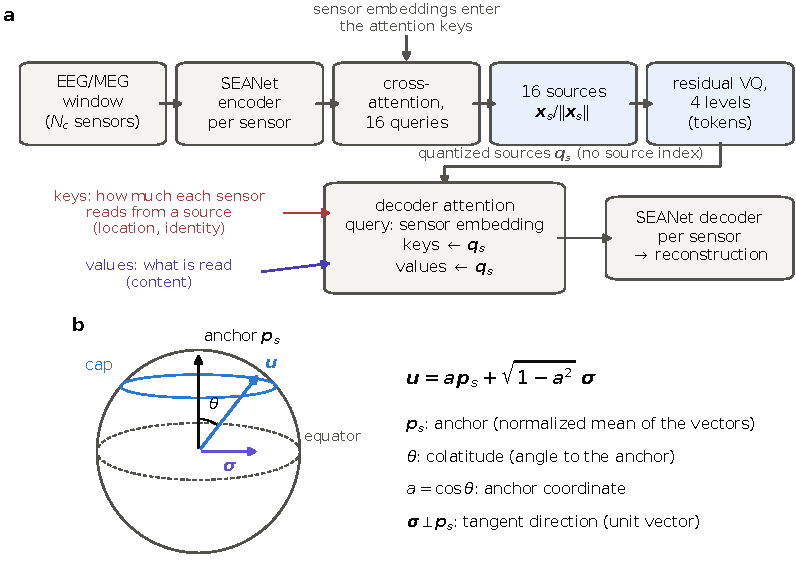
\includegraphics[width=\linewidth]{fig_overview.pdf}
\caption{(a)~The BrainOmni tokenizer. Every sensor's window is encoded separately; 16 learned queries
  pool the sensors into 16 latent sources (the sensor embeddings enter the keys of this
  cross-attention), whose unit vectors are quantized by a four-level residual
  vector quantizer. The decoder lets each sensor's embedding attend over the quantized sources: the
  attention keys, computed from the quantized vectors, determine how much each sensor reads from each
  source, and the values determine what is read. The decoder receives no source index, so the
  sources can be told apart only through their quantized vectors. (b)~Hyperspherical coordinates of
  the unit vectors $\uvec$ of one source: the anchor $\anchor_s$ (the normalized mean of the vectors),
  the colatitude $\theta$ (the angle to the anchor), the anchor coordinate $a=\cos\theta$ and the
  tangent direction $\bm{\sigma}$; the vectors of a source lie in a cap around its anchor.}
\label{fig:overview}
\end{figure}

\paragraph{Input} In the BrainOmni pipeline for downstream data, a recording with $N_c$
sensors is notch filtered at the mains frequency, band-pass filtered (0.1--96~Hz), resampled
to 256~Hz and cut into non-overlapping segments (10~s for EEG and 30~s for MEG; we used 10~s
throughout, \cref{sec:methods-data}); in every segment, the across-sensor mean
is subtracted at every sample and the data are divided by their global standard deviation,
separately for each sensor type \citep{brainomni2025}. (The pretraining data were processed
in the same way, except that they were notch filtered at both 50 and 60~Hz, resampled before
band-pass filtering, had bad EEG channels interpolated, and had the positions of all MEG sensors
normalized, whereas the downstream scripts normalize only those of magnetometers.) Every sensor
$c$ has a six-dimensional descriptor (its position, centered and scaled per modality, and its
orientation, which is zero for EEG) and a type (EEG, magnetometer or gradiometer), which a
small network maps to a sensor embedding $\bm{e}_c\in\R^{256}$.
The tokenizer processes 2-s windows (512 samples) independently; a 10-s segment
contains five windows.

\paragraph{Encoder and latent sources} A convolutional encoder with a residual two-layer long
short-term memory (LSTM) network \citep[SEANet, total stride 64;][]{soundstream2021,encodec2022} maps the window of each sensor
to $F=8$ frames of 256-dimensional features $\bm{h}_{c,f}$. For every frame, 16 learned query vectors
$\bm{n}_1,\dots,\bm{n}_{16}$ attend over the sensors through four-head cross-attention
whose keys are computed from $\bm{h}_{c,f}+\bm{e}_c$ and whose values are computed from
$\bm{h}_{c,f}$,
\begin{equation}
\begin{split}
  \bm{x}_{s,f} &= W_o\,\mathrm{Attn}\bigl(\bm{n}_s;\,\{\bm{k}_{c,f},\,\bm{z}_{c,f}\}_{c=1}^{N_c}\bigr)
  +\bm{b}_o\in\R^{256},\qquad s=1,\dots,16,\\
  \bm{k}_{c,f} &= W_k(\bm{h}_{c,f}+\bm{e}_c)+\bm{b}_k,\qquad \bm{z}_{c,f}=W_v\bm{h}_{c,f}+\bm{b}_v .
\end{split}
\end{equation}
We call $\bm{x}_{s,f}$ the vector of \emph{source} $s$ at frame $f$. Because the number
of queries is fixed, the representation has the same shape for every montage and
modality.

\paragraph{Quantizer} Each source vector is normalized,
$\uvec=\bm{x}/\lVert\bm{x}\rVert$, and quantized by a four-level residual vector
quantizer: level $\ell$ replaces the current residual by its nearest codeword
$\bm{c}_\ell$ in a codebook of 512 entries and passes on the difference, so that the
quantized vector is $\bm{q}=\sum_{\ell=1}^{4}\bm{c}_\ell$. The four codebooks are
shared by all sources and were learned with exponential-moving-average $k$-means
updates. The norm $\lVert\bm{x}\rVert$ is discarded: the tokenizer passes on only the
direction of each source vector, through its four code indices.

\paragraph{Decoder and objective} For every frame, the decoder lets the embedding of
each sensor attend over the 16 quantized sources (four-head attention with the sensor
embedding as query, and keys and values that are affine functions of the quantized
source vectors) and maps the result back to that sensor's waveform with a convolutional
decoder that mirrors the encoder. The decoder receives no source index or source
embedding, so it can tell the sources apart only through their quantized vectors; and it
reconstructs every sensor from that sensor's embedding and
the quantized sources alone, independently of the other sensors. The tokenizer was
trained to reconstruct all sensors of a window, z-scored per sensor and window, while
its encoder saw a random 75\% of the sensors with additive Gaussian noise. The loss is
the sum of the mean absolute error, $\exp(-r)$ with $r$ the mean Pearson correlation
between reconstructed and target waveforms, the mean absolute errors of the spectral
amplitude and (weighted by 0.5) of the spectral phase, and the commitment term of the
quantizer \citep{brainomni2025}. The tokenizer has \NumParams{} trainable parameters.

\paragraph{Tokenizer instances} We analyze (i)~the released BrainTokenizer checkpoint;
(ii)~the tokenizer stored inside the released BrainOmni foundation-model checkpoints
(identical in the \emph{tiny} and \emph{base} models), whose encoder and decoder equal
those of (i) up to bfloat16 rounding but whose codebooks differ; (iii)~\NumReplicas{}
tokenizers trained from scratch with the released architecture and objective
(\cref{sec:methods-replicas}), \NumVariants{} of them with a learned source embedding added to the
decoder's input; and, as a control for geometry only, (iv)~untrained tokenizers with
random weights. Unless stated otherwise, results refer to (i).

%% =========================================================================
\section{Methods}\label{sec:methods}

\subsection{Cohorts and preprocessing}\label{sec:methods-data}

We used four public OpenNeuro datasets \citep{markiewicz2021openneuro}
(\cref{tab:cohorts}): resting-state EEG from patients with Parkinson's disease off
medication and healthy controls recorded at UC San Diego
\citep[ds002778;][]{ds002778,jackson2019waveform,swann2015synchrony,george2013dopaminergic}
(\emph{PD-UCSD}); eyes-open resting-state EEG from patients with Parkinson's disease and
controls recorded at the University of Iowa \citep[ds004584;][]{ds004584,singh2023evoked,anjum2024resting}
(\emph{PD-Iowa}); eyes-closed resting-state EEG from patients with Alzheimer's disease,
frontotemporal dementia and cognitively normal controls
\citep[ds004504;][]{miltiadous2026ahepa,ds004504,miltiadous2023dicenet,miltiadous2023dataset} (\emph{Dementia}); and
resting-state MEG from adolescents with major depressive disorder and healthy
volunteers \citep[ds003568;][]{ds003568,liuzzi2022meg} (\emph{MDD-MEG}). All subjects
with a usable recording were included; PD-UCSD patients contributed their
off-medication session, and one PD-Iowa recording was excluded because its median
channel standard deviation exceeded 500~\textmu V. For MDD-MEG, the first 190~s of each resting recording (310--600~s
long) were read and filtered, and its first 18 complete segments (the first 180~s) were analyzed.

\begin{table}[tbp]
\renewcommand{\baselinestretch}{1}
\caption{Cohorts. All recordings are resting state (PD-Iowa eyes open, Dementia eyes closed); segments are non-overlapping 10-s sections of a recording (five 2-s tokenizer windows each); group sizes count the subjects analyzed. HC: healthy controls; PD: Parkinson's disease; CN: cognitively normal; AD: Alzheimer's disease; FTD: frontotemporal dementia; HV: healthy volunteers; MDD: major depressive disorder.}
\label{tab:cohorts}
\centering\scriptsize
\setlength{\tabcolsep}{4pt}
\begin{tabular}{@{}lllrrr@{\hspace{6pt}}l@{}}
\toprule
\textbf{cohort} & \textbf{accession} & \textbf{modality} & \textbf{sensors} & \textbf{subjects} & \textbf{segments} & \textbf{groups} \\
\midrule
PD-UCSD & ds002778 & EEG & 32 & 31 & 591 & HC 16, PD 15 \\
PD-Iowa & ds004584 & EEG & 60 & 148 & 2{,}167 & HC 49, PD 99 \\
Dementia & ds004504 & EEG & 19 & 88 & 7{,}013 & CN 29, AD 36, FTD 23 \\
MDD-MEG & ds003568 & MEG & 269 & 49 & 882 & HV 20, MDD 29 \\
\bottomrule
\end{tabular}
\end{table}


Preprocessing followed the BrainOmni pipeline for downstream data: notch filtering at the
mains frequency, 0.1--96~Hz band-pass filtering, resampling to 256~Hz, non-overlapping 10-s
segments and per-segment normalization as described in \cref{sec:background}. No artifact
rejection was applied: segments overlapping intervals annotated as bad or as recording boundaries
would have been discarded, but the only such annotation was the boundary event at the start of every
PD-Iowa recording, so the first 10~s of the PD-Iowa recordings were not used. EEG sensors were matched to the standard 10--05 or BioSemi template positions and
restricted to the channels shared by all recordings of a cohort; MEG used 269 of the 272 axial
gradiometers (three excluded by the fixed list of the BrainOmni MEG pipeline) after third-order
gradient compensation. For MEG we departed from the downstream pipeline in two respects:
segments were 10~s instead of 30~s long, as for EEG, and the positions of all MEG sensors were
normalized, as in the tokenizer's pretraining. Throughout, \emph{segment} refers to a retained 10-s segment and
\emph{window} to one of its five 2-s tokenizer inputs. Preprocessing was performed with
MNE-Python \citep{gramfort2013mne} on data organized in the Brain Imaging Data Structure (BIDS)
\citep{pernet2019eegbids,niso2018megbids,appelhoff2019mnebids}.

\subsection{Per-source unit vectors and anchor geometry}\label{sec:methods-geometry}

A segment yields $5\times8=40$ unit vectors per source (five windows of eight frames).
For source $s$ of a cohort, let $\uvec$ denote a random unit vector of that source,
drawn uniformly from its vectors in all segments used for the estimate. We define the
directional mean, its \emph{mean resultant length} and the \emph{anchor}
(\cref{fig:overview}b),
\begin{equation}
  \bm{\mu}_s=\E[\uvec],\qquad \Rbar_s=\lVert\bm{\mu}_s\rVert\in[0,1],\qquad
  \anchor_s=\bm{\mu}_s/\Rbar_s ,
\end{equation}
which are the standard location and concentration parameters of directional data
\citep{mardia2000directional}. Every unit vector has hyperspherical coordinates relative
to the anchor,
\begin{equation}\label{eq:coords}
  \uvec=a\,\anchor_s+\sqrt{1-a^{2}}\;\bm{\sigma},\qquad
  a=\langle\uvec,\anchor_s\rangle=\cos\theta,\qquad
  \bm{\sigma}\perp\anchor_s,\ \lVert\bm{\sigma}\rVert=1 ,
\end{equation}
consisting of the \emph{anchor coordinate} $a$ (equivalently the \emph{colatitude}
$\theta$, the angle between $\uvec$ and the anchor) and the \emph{tangent direction}
$\bm{\sigma}$; we write $\tvec=\uvec-a\anchor_s=\sqrt{1-a^{2}}\,\bm{\sigma}$ for the
tangent part. Note that $\E[a]=\Rbar_s$. Three kinds of principal directions are
distinguished. The \emph{uncentered principal directions} are the eigenvectors of the
second-moment matrix $M_s=\E[\uvec\uvec^{\top}]$; the \emph{centered principal
components} (PCs) are those of the covariance $\Sigma_s=M_s-\bm{\mu}_s\bm{\mu}_s^{\top}$;
and the \emph{tangent principal axes} are the eigenvectors of the covariance of the
tangent direction $\bm{\sigma}$, which lie in the hyperplane orthogonal to the anchor.
The following proposition relates the anchor to the leading uncentered direction
$\bm{v}_1$ of $M_s$; it combines elementary identities with the residual form of the Davis--Kahan
$\sin\Theta$ theorem \citep{davis1970rotation} and Weyl's inequality (proof in \cref{app:proof}). We write $\lambda_1\geq\lambda_2\geq\dots$
for the eigenvalues of $M_s$ and $\bm{\gamma}_s=\operatorname{Cov}(a,\tvec)=\E[a\tvec]$ for the
cross-covariance between the anchor coordinate and the tangent part.

\begin{proposition}\label{prop:anchor}
For unit vectors with $\Rbar_s>0$:
\begin{enumerate}
\item[(i)] $M_s\anchor_s=\E[a^{2}]\,\anchor_s+\bm{\gamma}_s$ with $\bm{\gamma}_s\perp\anchor_s$;
  in particular, $\anchor_s^{\top}M_s\anchor_s=\E[a^{2}]$, and $\anchor_s$ is an eigenvector of
  $M_s$ if and only if $\bm{\gamma}_s=\bm{0}$.
\item[(ii)] If $\E[a^{2}]>\lambda_2$, then, for $\bm{v}_1$ oriented so that
  $\langle\bm{v}_1,\anchor_s\rangle\geq0$,
  \begin{equation}\label{eq:residual-bound}
    \sin\angle(\bm{v}_1,\anchor_s)\;\leq\;\frac{\lVert\bm{\gamma}_s\rVert}{\E[a^{2}]-\lambda_2}\,.
  \end{equation}
\item[(iii)] $\lambda_2\leq\lVert\Sigma_s\rVert_{\mathrm{op}}$, so (ii) also holds with
  $\lambda_2$ replaced by $\lVert\Sigma_s\rVert_{\mathrm{op}}$ whenever
  $\E[a^{2}]>\lVert\Sigma_s\rVert_{\mathrm{op}}$.
\item[(iv)] $\lVert\bm{\gamma}_s\rVert\leq\sqrt{\operatorname{Var}(a)\,\lVert\Sigma_s\rVert_{\mathrm{op}}}$,
  so the right-hand side of~\eqref{eq:residual-bound} is at most
  $\sqrt{\operatorname{Var}(a)\,\lVert\Sigma_s\rVert_{\mathrm{op}}}\,/\,(\E[a^{2}]-\lambda_2)$.
\item[(v)] $\operatorname{tr}\Sigma_s=1-\Rbar_s^{2}$ and
  $\Sigma_s\anchor_s=\operatorname{Var}(a)\,\anchor_s+\bm{\gamma}_s$; in particular, the variance
  along the anchor is $\anchor_s^{\top}\Sigma_s\anchor_s=\operatorname{Var}(a)=\E[a^{2}]-\Rbar_s^{2}$.
\end{enumerate}
\end{proposition}

By (i), the anchor is an exact eigenvector of $M_s$ exactly when the anchor coordinate is
uncorrelated with the tangent part, and by (ii) it stays close to the leading eigenvector as
long as the norm of their cross-covariance is small compared with the gap between $\E[a^{2}]$
and the second eigenvalue. By (iv), this is guaranteed whenever the anchor coordinate varies
little, whatever its correlation with the tangent part: concentration in colatitude together
with an eigengap suffices. The classical perturbation bound
$\sin\angle(\bm{v}_1,\anchor_s)\leq2\lVert\Sigma_s\rVert_{\mathrm{op}}/\Rbar_s^{2}$
\citep{davis1970rotation,yu2015daviskahan}, which treats all of $\Sigma_s$ as a perturbation of
$\bm{\mu}_s\bm{\mu}_s^{\top}$, is much weaker because it ignores that most of the variation is
tangential. By (i) and (v), the anchor satisfies the eigenvalue equations of both second moments
up to the same residual $\bm{\gamma}_s$: that of $M_s$ with the Rayleigh quotient $\E[a^{2}]$,
which under the condition of (ii) lies between $\lambda_2$ and $\lambda_1$, and that of $\Sigma_s$
with the Rayleigh quotient $\operatorname{Var}(a)$, which may be a small share of
$\operatorname{tr}\Sigma_s$. The anchor can therefore be the leading uncentered
direction without being a leading centered one. Whether it is close to a single eigenvector depends
on the distance from the corresponding eigenvalue to the others: for $M_s$ this is the eigengap of
(ii); applied to $\Sigma_s$, the same argument guarantees closeness to a single centered PC only if
$\lVert\bm{\gamma}_s\rVert$ is small compared with the distance from $\operatorname{Var}(a)$ to the
neighboring eigenvalues of $\Sigma_s$, and otherwise the anchor can be spread over several
centered PCs of similar variance.

For every source we report $\Rbar_s$; the mean colatitude; $\cos\angle(\bm{v}_1,\anchor_s)$
together with the bound~\eqref{eq:residual-bound}, its versions (iii) and (iv) and the
classical bound; the absolute cosine between the anchor and each of the ten leading centered PCs,
and the largest absolute cosine between the anchor and any of the 64 leading centered PCs together
with the rank of that PC;
the squared norm of the projection of the anchor onto the span of the $k$ leading centered
PCs ($k=10,16,64$); the share of $\operatorname{tr}\Sigma_s$ along the anchor and its rank
among the eigenvalues of $\Sigma_s$; the participation ratio
$(\operatorname{tr}\Sigma_s)^2/\operatorname{tr}(\Sigma_s^2)$ as an effective
dimensionality of the variation; and the share of the variance of the tangent direction
captured by its 16 and 64 leading tangent axes. For the anchors of all 16 sources together, we
report how many directions they span, as the participation ratio of the eigenvalues of their
cosine matrix $G_{ss'}=\langle\anchor_s,\anchor_{s'}\rangle$ (the cumulative shares of these
eigenvalues are the fractions of the anchors' squared norm in their leading principal directions),
and the smallest angle between two anchors. When the two leading eigenvalues of $G$ hold at least
99\% of their sum, we also report the gaps between consecutive anchors along the circle, the
differences between the polar angles of the anchors projected onto the plane of the two leading
eigenvectors of $G$. Geometry was estimated from the second to
fourth segment of every recording ($120$ vectors per subject and source; the first segment
was excluded to avoid filter transients). Reliability was assessed by split halves over
subjects (30 random splits), by the agreement of each subject's anchor with the anchor of
the remaining subjects, and by the agreement of anchors estimated on different cohorts.
Intervals are 95\% subject-cluster bootstrap intervals (200 resamples).

\subsection{Interventions}\label{sec:methods-interventions}

To measure which aspects of a source the decoder relies on, we edit the unit vectors of one
source in a segment, re-run the frozen quantizer and decoder, and record the change in
reconstruction error (mean squared error, MSE) relative to the unedited reconstruction,
\begin{equation}
  \dmse=\mathrm{MSE}\bigl(\hat{X}_{\text{edit}},X\bigr)-\mathrm{MSE}\bigl(\hat{X},X\bigr),
\end{equation}
where $X$ is the tokenizer's training target (each sensor and window z-scored) and the error is
averaged over sensors, windows and samples; we report $\dmse$ mostly in percent of the unedited
error of the segment, and compute the change in mean absolute error ($\Delta$MAE) and in one
minus the mean Pearson correlation between reconstructed and target waveforms ($\Delta(1-r)$)
in the same way. Because the quantizer normalizes its input, edits that move vectors off the
unit sphere---such as scaling or averaging the coordinate along a direction---would be partly
undone by the normalization before they reached the codebooks: halving the anchor component of
every vector without renormalizing would, after the quantizer's normalization, have achieved only
\OffSphereHalfMin--\OffSphereHalfMax\% of the intended change in the anchor coordinate (median over
the vectors of a source), and setting it to its mean would have left \OffSphereMeanLeftMin--%
\OffSphereMeanLeftMax\% of the variance of the anchor coordinate. All edits are therefore defined
in the hyperspherical coordinates of \cref{eq:coords} and map unit vectors to unit vectors
(\cref{tab:operators}). They separate three aspects of a source. \emph{Location} edits
change the anchor coordinate and keep the tangent direction: setting it to zero (\emph{zero-anchor}: moving every
vector to the anchor's equator; this equals projection, or zero, ablation of the anchor
followed by the quantizer's normalization), halving it, replacing it by its mean or by the
coordinate of a randomly permuted vector of the same segment, and shifting the colatitude by
$\pm10^\circ$ or $\pm20^\circ$ (vectors closer to the anchor than a negative shift are moved onto
it). \emph{Content} edits keep the anchor coordinate and change the
tangent direction: replacing its components on the $k$ leading tangent axes by those of the
vector at the same position in a segment from another subject (resample ablation;
$k=1,4,16,64$), by those of the mean of the tangent directions, $\E[\bm{\sigma}]$, which is
not normalized and short, so that this nearly zeroes these components before renormalization
(mean ablation; $k=1,4$), or replacing the whole tangent direction. As controls, the same resample ablation was applied to $k$ random
orthonormal directions inside the span of the 64 leading tangent axes, which contains almost
all of the tangent variance (the \emph{support}; $k=1,4,16$), and to 16 random directions of
the whole tangent space (orthogonal to the anchor, with on average a quarter of their squared
norm in the support); and the tangent direction was rotated by a fixed angle or by a per-vector
angle chosen such that the geodesic displacement equals that of zero-anchor (\emph{matched
rotation}). A matched rotation keeps the colatitude and moves each vector by the same angle as
zero-anchor, around the anchor instead of towards its equator, which separates the effect of
the direction of an edit from that of its size; for vectors within $30^\circ$ of the anchor
(a median of \WithinThirtyMedianPct\% and at most \WithinThirtyMaxPct\% of the vectors of a
source), no such angle exists and the rotation is by $180^\circ$. The \emph{source-identity}
edit rotates all vectors of a source in the plane spanned by its anchor and the anchor of
another source so that its anchor is mapped onto the other one (\emph{anchor swap}), which
preserves every angle within the source. As an extreme, \emph{collapse} replaces every vector
by the anchor, which removes all content and sets the colatitude to zero while keeping the anchor, and \emph{source resample}
replaces all vectors of a source by those of a segment from another subject, which gives a
reference level for the damage caused by replacing a source with realistic content.

\begin{table}[tbp]
\renewcommand{\baselinestretch}{1}
\caption{Edits applied to the unit vectors of one source, in the hyperspherical coordinates
  of \cref{eq:coords} (anchor $\anchor$, anchor coordinate $a=\cos\theta$, tangent direction
  $\bm{\sigma}\perp\anchor$). Every edit maps unit vectors to unit vectors. $\bm{\sigma}'$ and
  $\uvec'$ denote the tangent direction and the unit vector at the same position of a segment
  from another subject; the \emph{support} is the span of the 64 leading tangent axes.
  Statistics ($\anchor$, $\bar{a}$, tangent axes, mean of the tangent directions) are cross-fitted
  (\cref{sec:methods-interventions}). Routing: zero-anchor, the anchor swap, tangent resample and
  tangent-axis resample (4) were also applied only to the input of the decoder's attention keys, or
  only to that of its values.}
\label{tab:operators}
\centering\footnotesize
\setlength{\tabcolsep}{3pt}
\begin{tabular}{@{}>{\raggedright\arraybackslash}p{0.27\linewidth}>{\raggedright\arraybackslash}p{0.42\linewidth}>{\raggedright\arraybackslash}p{0.27\linewidth}@{}}
\toprule
\textbf{edit} & \textbf{definition} & \textbf{changes} \\
\midrule
\multicolumn{3}{@{}l}{\emph{Location: $\bm{\sigma}$ kept}} \\
zero-anchor          & $a\leftarrow0$ ($\theta\leftarrow90^\circ$)                         & colatitude \\
half-anchor          & $a\leftarrow a/2$                                                   & colatitude \\
mean-anchor          & $a\leftarrow\bar{a}$ (mean anchor coordinate)                        & colatitude variation \\
resample-anchor      & $a\leftarrow$ coordinates randomly permuted among the vectors of the segment & pairing of $a$ and $\bm{\sigma}$ \\
colatitude shift     & $\theta\leftarrow\min\{\max(\theta+\delta,0^\circ),180^\circ\}$, $\delta\in\{\pm10^\circ,\pm20^\circ\}$ (clipped at the anchor) & colatitude \\
\multicolumn{3}{@{}l}{\emph{Content: $a$ kept}} \\
tangent-axis resample ($k$) & components of $\bm{\sigma}$ on the $k$ leading tangent axes $\leftarrow$ those of $\bm{\sigma}'$; renormalized & content in the leading axes \\
tangent-axis mean ($k$) & as above with the mean $\E[\bm{\sigma}]$ of the tangent directions (not normalized) instead of $\bm{\sigma}'$ & content in the leading axes \\
random-support resample ($k$) & as tangent-axis resample, $k$ random orthonormal directions of the support & content in a random subspace \\
random resample (16) & as above, 16 random directions of the whole tangent space ($\perp\anchor$) & content in a random subspace \\
tangent resample     & $\bm{\sigma}\leftarrow\bm{\sigma}'$                                  & all content \\
matched rotation     & $\bm{\sigma}\leftarrow\cos\psi\,\bm{\sigma}+\sin\psi\,\bm{\xi}$, $\bm{\xi}\perp\bm{\sigma}$ random in the support (or in $\anchor^{\perp}$), $\psi$ giving zero-anchor's displacement ($\psi=180^\circ$ within $30^\circ$ of $\anchor$) & content, at equal displacement \\
rotation ($\psi$)    & as above with $\psi=30^\circ,60^\circ,90^\circ$, $\bm{\xi}$ in the support & content \\
\multicolumn{3}{@{}l}{\emph{Source identity and whole source}} \\
anchor swap          & rotation in $\operatorname{span}\{\anchor_s,\anchor_{s'}\}$ taking $\anchor_s$ to the anchor $\anchor_{s'}$ of another source & which anchor \\
collapse             & $\uvec\leftarrow\anchor$                                            & all content and colatitude \\
source resample      & $\uvec\leftarrow\uvec'$                                             & everything \\
\bottomrule
\end{tabular}
\end{table}


To locate these effects in the decoder, we applied zero-anchor and the anchor swap to only
one of the two pathways through which the quantized sources enter the decoder's attention:
the input of its keys (which determine how much each sensor reads from each source) or that of
its values (what is read), the other pathway receiving the unedited quantized vectors. A second
run on the same segments applied the same split to zero-anchor, to the anchor swap, to the
resample of the whole tangent direction and to the resample of the four leading tangent axes; the
key and value shares plotted for these four edits (\cref{sec:res-routing}) and the routing of the
content edits reported there come from this run, all other zero-anchor and swap values from the first (the
two runs gave the same zero-anchor shares and swap shares within 0.01). For
zero-anchor we also recorded the attention weight that the sensors assign to the edited source,
averaged over sensors, heads and frames.

Anchors, mean anchor coordinates, mean tangent directions and tangent axes were cross-fitted:
subjects were split at random into two halves, and the segments of each half were edited with
statistics estimated on the other. Edits were applied to every source of two segments per
subject in PD-UCSD and MDD-MEG (the third and the seventh segment of the recording) and of one
segment per subject in the larger PD-Iowa and Dementia cohorts (the third). Segments were
processed in groups of 16 (8 for MDD-MEG), each containing segments of at least two subjects,
from which the donor segments of the resample edits were drawn (one random assignment of every
segment to a segment of another subject per group, shared by all sources and all resample edits,
so that comparisons between edits are paired). For every source and group,
three partner sources were drawn for the anchor swap (the split into keys and values used the
first), two random support subspaces of each dimension, one random 16-dimensional subspace of
the tangent space, and one random rotation direction for every vector. For the 60- and
269-channel cohorts the reconstruction was evaluated on a fixed random subset of 32 sensors,
which is exact for the sampled sensors because the decoder reconstructs every sensor
independently of the others (\cref{sec:background}); the encoder always saw all sensors.
Results were averaged per subject (over segments and draws); for every source we report the
mean over subjects, with a 95\% subject-cluster bootstrap interval (2000 resamples), and
differences and ratios between edits are computed from the subject means with the same
resamples (paired bootstrap). We call an effect \emph{positive for a source} when the interval of
its subject-mean $\dmse$ lies above zero; these counts, and the differences and ratios between
edits, are computed from $\dmse$ itself; values given in percent of the unedited error use the change
relative to the unedited error of each segment, and shares between edits are ratios of $\dmse$.

\subsection{Token analysis}\label{sec:methods-tokens}

For every RVQ level $\ell$ and cohort we computed, over the vectors of all segments, the
mutual information $I(S;C_\ell)$ between the source index $S$ and the code $C_\ell$ in bits
(with 16 equally frequent sources, $H(S)=4$~bits), its share of the entropy of the code, the
accuracy of identifying the source from the code alone (each code assigned to the source that
uses it most often), and the perplexity of the code usage of every source. For level~1 we
computed the usage-weighted cosine between the codewords a source selects and its anchor. We
then re-quantized the vectors used for the geometry after editing them as in
\cref{tab:operators} (with statistics estimated on the same vectors and donor tangent
directions taken from a random segment of another subject), and recorded the fraction of
vectors whose level-1 code changed, the fraction of these changes that went to a code used
most often by another source, and, among vectors whose level-1 code did not change, the
fraction whose level-2 code changed.

\subsection{Independently trained tokenizers}\label{sec:methods-replicas}

To test whether the findings depend on one trained checkpoint, we trained tokenizers from
scratch with the released architecture (16 sources, four codebooks of 512 entries) and
objective (reconstruction of all sensors from 75\% of them, with the loss of
\cref{sec:background}; input noise of standard deviation 0.1, commitment term 0.25 times the
mean squared quantization error averaged over levels, codebooks updated by the moving-average
rule with decay 0.99 and initialized by $k$-means on the first batch, codewords whose moving-average
usage count fell below 2 re-initialized) and with the released optimizer (AdamW with $\beta=(0.5,0.9)$,
$\epsilon=10^{-5}$, learning rate $2\times10^{-4}$, weight decay 0.01 except for normalization
weights and the sensor-type embedding; cosine decay of the learning rate to 0.05 times its
initial value after a warm-up over 10\% of the steps). The subjects of every cohort were split,
stratified by group, into a training set (75\%) and a held-out set (25\%; \RepHeldOutUCSD,
\RepHeldOutIowa, \RepHeldOutDementia{} and \RepHeldOutMEG{} subjects in PD-UCSD, PD-Iowa, Dementia
and MDD-MEG); the same split was used for all tokenizers we trained, and every analysis of them
used held-out subjects only. Each training step drew one cohort at random and a batch of eight
ten-second segments, with replacement, from its training subjects, restricted to one random subset
of 16 EEG or 32 MEG sensors shared by the segments of the step; because the decoder reconstructs
every sensor independently of the others (\cref{sec:background}), a sensor subset is a valid
training input. Training ran for \ReplicaSteps{} steps. \NumSeedReplicas{} tokenizers
(\emph{replicas}; replica~$k$ uses seed~$k$) differ only in their random seed. \VariantCountCap{} further tokenizers use the seeds of
the replicas, so that their initial weights (apart from the added embedding) and their sequences of
training batches equal those of the replicas, and add a learned embedding $\bm{\eta}_s\in\R^{256}$ of
each source, initialized from a truncated normal distribution with variance $1/256$, to the quantized
source vectors before the decoder's key and value projections (\emph{source-embedding variants};
variant~$k$ uses the seed of replica~$k$). The
variants give the decoder a second way to identify the sources, independent of their direction, and
therefore test whether the role of the anchors depends on the decoder having no other access to
source identity, and each variant is compared with the replica of the same seed.

We made three changes to the published recipe. First, with the original
initialization all sources coincided (\cref{sec:res-geometry}) and, in a pilot run of
\ReplicaSteps{} steps with the recipe otherwise as for the replicas, did not separate
(held-out PD-UCSD: mean resultant length \PilotRbar, pairwise cosine between the anchors
$\geq$\,\PilotOffdiagMin; training-batch correlation between reconstructed and target waveforms
\PilotPCC{} at the end of training, against \RepPCC{} for replica~1); we therefore initialized the convolution biases of the encoder and decoder to zero
and drew the weights of the sensor-position network and of the encoder's attention keys with
standard deviation 0.2 instead of 0.02. Second, the codebook implementation re-initializes unused
codewords from the current batch, but the replacement is overwritten by the following
moving-average update; we made the replacement effective. Third, for numerical stability, we clipped the gradient norm at 1,
trained in single precision instead of bfloat16, and used a linear instead of the released
logarithmic warm-up. The training data comprised \ReplicaHours{}~h of recordings, a small fraction
of the corpus of the released tokenizer, and the batch was eight segments on sensor subsets instead
of the 512 full segments of the released training. The replicas therefore test whether the geometry
and its causal roles emerge from the architecture and objective under a modified initialization
and a much smaller training budget, not whether the released tokenizer's reconstruction quality can
be reached. We report their reconstruction error on held-out subjects next to that of the released
tokenizer, and the geometry of the first replica at initialization as an untrained control.
Geometry, tokens and interventions were analyzed as for the released tokenizer, on the held-out
subjects, except that intervention segments were processed in groups of eight in every cohort and
that one random support subspace of each dimension and one random 16-dimensional subspace were
drawn per group and source; the held-out sets are small (8 to 37 subjects), so the subject-cluster
intervals of these tokenizers are approximate. Because the caps of the replicas are narrow
(\cref{sec:res-replication}; a median of \RepWithinThirtyMedianPct\% of the vectors of a source lie
within $30^\circ$ of the anchor), the matched rotation is the $180^\circ$ fallback for most of their
vectors and moves them less than zero-anchor, shifts of the colatitude towards the anchor move many
vectors onto it, and halving the anchor component off the sphere would have achieved only
\RepOffSphereHalfMin--\RepOffSphereHalfMax\% of the intended change.

\subsection{Diagnostic read-out}\label{sec:methods-readout}

For every subject, per-segment quantities were averaged over all of the subject's
segments. The primary representation was the vector of the 16 anchor coordinates
$\langle\bar{\uvec}_s,\anchor_s\rangle$, where $\bar{\uvec}_s$ is the subject's mean unit vector
of source $s$ (\emph{anchor-16}). Secondary representations were the full
per-source representation $(\bar{\uvec}_1,\dots,\bar{\uvec}_{16})\in\R^{4096}$
(\emph{full}); the same with the anchor coordinates removed (\emph{tangent}); the mean over
sources (\emph{pooled}, 256-D); the per-source means of the quantized vectors $\bm{q}$, the
tokenizer's output (\emph{quantized}, 4096-D), and their anchor coordinates (\emph{quantized
anchor-16}); the mean resultant lengths of the vectors of each source within a segment
(\emph{concentration-16}); the mean norms before normalization, which the quantizer discards
(\emph{norm-16}); and log band power in five bands (1--4, 4--8, 8--13, 13--30, 30--45~Hz) per
sensor, computed from the preprocessed segments (average-referenced and scaled by their global
standard deviation, so that it measures relative power). Anchors were re-estimated on the
training subjects of every cross-validation fold.

Classification used L2-regularized logistic regression on standardized features (for
high-dimensional representations the standardized training data were first rotated onto their
non-degenerate principal axes, which is lossless for an L2 penalty). The inverse regularization
strength was chosen from 13 log-spaced values between $10^{-4}$ and $10^{2}$ by the AUC of an
inner stratified five-fold cross-validation on the training subjects, and the model was then
refitted on all training subjects. Performance is the AUC in stratified five-fold cross-validation repeated 20 times: in every
repetition the out-of-fold scores of all subjects were pooled over the five folds and one AUC was
computed, and we report the mean over repetitions. Its interval is a 95\% stratified bootstrap
over subjects of the same statistic with the out-of-fold scores held fixed (2000 resamples); it
describes the uncertainty of evaluating the fitted classifiers on these subjects, not that of the
cross-validated AUC, and inference rests on permutation tests. $P$-values for AUCs above chance were obtained by
permuting the diagnostic labels across subjects and re-running the entire cross-validation,
$p=(1+\#\{\text{null}\geq\text{observed}\})/(1+n_{\text{perm}})$; because nested selection of the
regularization strength inside every permutation is costly, the permutation test uses the same
pipeline with the inverse regularization strength fixed at 1 and two repetitions, for the observed
and the permuted labels alike, which keeps the test exact for that pipeline (its statistic differed
from the reported AUC by at most \PermStatMaxDiff). The primary hypothesis (anchor-16 above chance) was tested
with 1000 permutations per contrast and Holm-corrected across the five contrasts
\citep{holm1979simple}; secondary representations were tested with 500 permutations and
Benjamini--Hochberg-corrected within each contrast \citep{benjamini1995fdr}. Single anchor
coordinates were read out with the inverse regularization strength fixed at 1 and tested with a
single-step maximum-statistic permutation test across the 16 sources of a contrast
\citep[1000 permutations;][]{westfall1993resampling}; in addition, a nested procedure selected,
inside every training fold, the anchor coordinate whose AUC on the training subjects was farthest
from 0.5 and evaluated it out of fold (\emph{best single anchor}; the selection was repeated inside
every one of 1000 permutations). As a null for anchor-16, the identical procedure was applied to
16 random unit directions (one per source; 100 draws), with the Monte Carlo $p$-value
$(1+\#\{\text{random}\geq\text{observed}\})/(1+n_{\text{rand}})$. Differences between representations were
assessed on the same subjects with a paired stratified bootstrap of the difference of their AUCs
(2000 resamples, out-of-fold scores held fixed), for every representation against band power and
against anchor-16; for this comparison the out-of-fold scores were recomputed with the same folds and
seeds, which reproduced the reported AUCs to within \PairedMaxDeviation. The $p$-value of a paired
difference is two-sided: twice the smaller of the fractions of bootstrap resamples in which the
difference is at most or at least zero. Like the intervals, these differences hold the out-of-fold
scores fixed and ignore the variability of model fitting, so they are descriptive rather than tests;
because every bootstrap resample averages the AUC over the 20 repetitions, their intervals narrow as
the out-of-fold predictions differ more between repetitions. To assess confounding by age and sex, we
evaluated a classifier on age and sex alone and repeated the analysis of anchor-16, the full
representation and band power with both regressed out of the features (least squares fitted on the
training subjects of every fold). These $p$-values, which are not corrected for multiple testing, come
from permuting the labels while age and sex stay with the features; they test the joint null that the
labels are independent of the features and of the covariates, and therefore do not isolate
information beyond age and sex.

To test transfer across sites and montages, a classifier was trained on all subjects of one
Parkinson's cohort and applied to all subjects of the other, which is possible because the source
representations have the same dimensionality for every montage (band power was restricted to the
\TransferSharedChannels{} electrodes shared by the two montages). Anchors were estimated on the
training cohort, and the regularization strength was chosen by stratified five-fold
cross-validation on it. Features were standardized with the training cohort's statistics or,
in a second analysis, within each cohort (a label-free harmonization). For every representation, the AUC of the
fitted classifier on the test cohort is given with a stratified bootstrap interval over the test
subjects (scores held fixed). Its $p$-value was obtained by permuting the labels of the test
cohort with the classifier fixed (10{,}000 permutations), which is exact under the null hypothesis
that the transferred scores are unrelated to the test labels; as within cohorts, the $p$-values of
anchor-16 were Holm-corrected across the two directions and those of the secondary
representations Benjamini--Hochberg-corrected within each direction. Each secondary representation
was compared with anchor-16 by a paired stratified bootstrap of the difference of their AUCs on the
test subjects (Holm-corrected across the eight comparisons of a direction), and every
representation with the AUCs of \TransferIowaToUCSDRandN{} random 16-direction representations
evaluated like anchor-16; for anchor-16 this gives a Monte Carlo $p$-value as within cohorts,
Holm-corrected across the two directions and, as a check, across both directions and both scalings.

\subsection{Software and reproducibility}

All analyses used PyTorch 2.11, scikit-learn 1.8 and MNE-Python 1.12 on a single Apple
M2 Pro computer. For every export and intervention run, GPU (Metal) results were checked against
CPU results on its first four segments: the unit vectors differed by at most $\DeviceUnitDiffMax\times10^{-6}$, and the
codes were identical for the released and embedded tokenizers and agreed for at least
\DeviceCodeReplicaMinPct\% of the vectors for the tokenizers we trained (the untrained controls,
whose codebooks are initialized from the first batch, were used for geometry only). Code, the
exact segment and subject lists, and the intermediate results needed to regenerate every number,
table and figure are available as described in the Data availability statement.

%% =========================================================================
\section{Results}\label{sec:results}

\subsection{Each source occupies a cap around a tokenizer-specific anchor}\label{sec:res-geometry}

\Cref{tab:geometry} and \cref{fig:geometry} summarize the geometry of the per-source unit
vectors. In every cohort, the vectors of every source were concentrated around their
anchor (\cref{fig:geometry}a): mean resultant lengths ranged from \RbarMinEEG{} to \RbarMaxEEG{} in the EEG
cohorts and from \RbarMinMEG{} to \RbarMaxMEG{} in MEG, and the mean colatitude ranged from
\AngleMin$^\circ$ to \AngleMax$^\circ$, whereas two independent random directions in 256
dimensions are $90^\circ$ apart to within a few degrees. Each source therefore occupies a
cap of the hypersphere around its anchor. The anchors were estimated precisely: anchors
computed from random halves of the subjects agreed to cosine $\geq$\,\SplitHalfMin{}, and
the anchor of a single subject agreed with that of the remaining subjects to a median cosine
of \LosoMedianMin--\LosoMedianMax{} across cohorts (5th percentiles
\LosoPfiveMin--\LosoPfiveMax). Anchors of different sources were
distinct but not orthogonal (pairwise cosines between \OffdiagMin{} and \OffdiagMax{},
median absolute cosine \OffdiagAbsMedian{}, compared with about 0.04 for random directions).
Together, the 16 anchors lay close to a four-dimensional subspace: their four leading principal
directions captured at least \AnchorFourShareMin\% of their summed squared norm (participation
ratio \AnchorDimMin--\AnchorDimMax), and the smallest angle between two anchors was
\AnchorMinAngleMin--\AnchorMinAngleMax$^\circ$.

The anchors of a source estimated on different cohorts were closely aligned
(\cref{fig:geometry}c): per-source cosines were at least \CrossCohortEEGMin{} among the
three EEG cohorts, which differ in site, montage (19 to 60 channels), population and
recording condition (angles of at most \CrossCohortEEGMaxAngle$^\circ$), and at least
\CrossModalMin{} between the EEG cohorts and MEG (at most \CrossModalMaxAngle$^\circ$), compared
with at least \AnchorMinAngleMin$^\circ$ between the anchors of different sources. The anchors are
therefore largely fixed by the tokenizer; the recording modality shifts them by up to
\CrossModalMaxAngle$^\circ$, less than the separation between the anchors of different sources. They
are a product of training: with the released initialization and random
weights, the vectors of all 16 sources pointed in one common direction (PD-UCSD; mean resultant length
\RandomRbar{}, pairwise cosine between the anchors $\geq$\,\RandomOffdiagMin{}; see also
\cref{sec:methods-replicas}), and the same held at the initialization used for the tokenizers we
trained (mean resultant length \InitRbar{}, pairwise cosine between the anchors
$\geq$\,\InitOffdiagMin{}).

\begin{table}[tbp]
\renewcommand{\baselinestretch}{1}
\caption{Geometry of the per-source unit vectors (released tokenizer); ranges over the 16 sources. $\Rbar$: mean resultant length; colat.: mean colatitude; $\cos(\anchor,\bm{v}_1)$: anchor versus leading uncentered direction; bound: residual bound~\eqref{eq:residual-bound} on $\sin\angle(\anchor,\bm{v}_1)$; $|\cos(\anchor,\mathrm{PC}_k)|$: largest absolute cosine with the ten leading centered PCs; $\|P_{16}\anchor\|^2$: squared norm of the anchor in the span of the 16 leading centered PCs; var.: share of the centered variance along the anchor (rank among the centered eigenvalues); PR: participation ratio of the centered covariance, $(\operatorname{tr}\Sigma_s)^2/\operatorname{tr}(\Sigma_s^2)$. Upper limits ($\leq$) are rounded up and lower limits ($\geq$) down. Per-source values, with a bootstrap interval for $\Rbar$, are given in \cref{app:tables}.}
\label{tab:geometry}
\centering\scriptsize
\setlength{\tabcolsep}{2.6pt}
\begin{tabular}{@{}lcccccccc@{}}
\toprule
\textbf{cohort} & $\Rbar$ & \textbf{colat.}\,($^\circ$) & $\cos(\anchor,\bm{v}_1)$ & \textbf{bound} & $|\cos(\anchor,\mathrm{PC}_k)|$ & $\|P_{16}\anchor\|^2$ & \textbf{var.} (\textbf{rank}) & \textbf{PR} \\
\midrule
PD-UCSD & 0.57--0.73 & 43--55 & $\geq$0.9986 & $\leq$0.054 & $\leq$0.50 & 0.24--0.83 & 2.2--3.5\% (12--18) & 16--21 \\
PD-Iowa & 0.58--0.70 & 45--54 & $\geq$0.9994 & $\leq$0.038 & $\leq$0.53 & 0.25--0.87 & 2.4--3.8\% (12--17) & 16--23 \\
Dementia & 0.49--0.65 & 49--60 & $\geq$0.9973 & $\leq$0.080 & $\leq$0.59 & 0.26--0.88 & 2.5--4.9\% (7--17) & 17--22 \\
MDD-MEG & 0.57--0.71 & 44--55 & $\geq$0.9995 & $\leq$0.035 & $\leq$0.40 & 0.13--0.40 & 1.3--1.8\% (16--22) & 17--20 \\
\bottomrule
\end{tabular}
\end{table}


\begin{figure}[tbp]
\centering
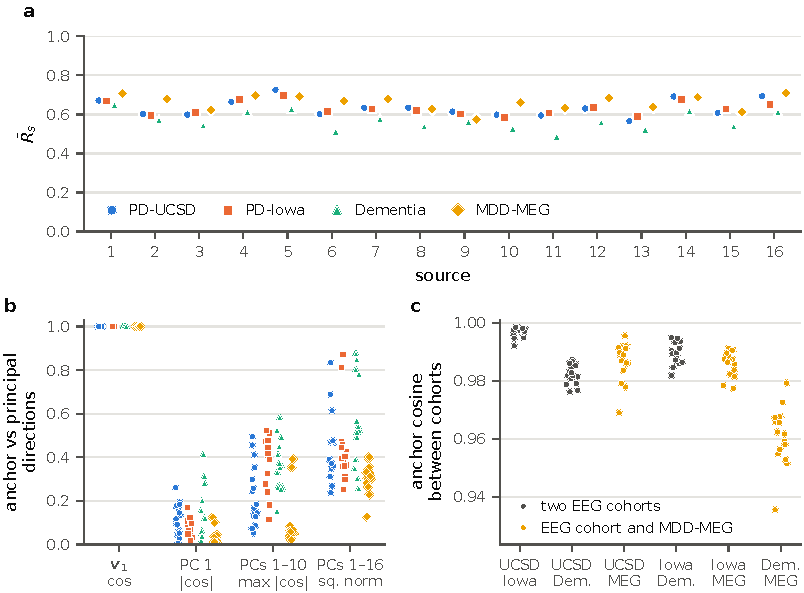
\includegraphics[width=\linewidth]{fig_geometry.pdf}
\caption{Geometry of the per-source unit vectors (released tokenizer). (a)~Mean resultant
  length $\Rbar_s$ of each source in each cohort. (b)~Anchor versus principal directions,
  one point per source and cohort: cosine with the leading uncentered direction $\bm{v}_1$;
  absolute cosine with the first centered PC; largest absolute cosine with any of the ten
  leading centered PCs; and squared norm of the anchor's projection onto the span of the 16
  leading centered PCs; colors and markers denote cohorts as in (a). (c)~Cosine between the anchors
  of the same source estimated on two different cohorts, for every pair of cohorts (UCSD: PD-UCSD,
  Iowa: PD-Iowa, Dem.: Dementia, MEG: MDD-MEG); one point per source; grey: two EEG cohorts, amber:
  an EEG cohort and MDD-MEG.}
\label{fig:geometry}
\end{figure}

\subsection{The anchor is the leading uncentered direction but not a leading centered one}\label{sec:res-pca}

For every source in every cohort, the anchor coincided with the leading eigenvector of the
uncentered second-moment matrix (cosine $\geq$\,\CosUncMin{}; \cref{fig:geometry}b). \Cref{prop:anchor}
accounts for this almost exactly: the observed sine of the angle (at most \SinUncMax{}) was a
median of \BoundTightnessMedian{} times the residual bound~\eqref{eq:residual-bound} (at most
\ResidualBoundMax{}), because the cross-covariance between the anchor coordinate and the tangent
part was small ($\lVert\bm{\gamma}_s\rVert$ between \CrossCovMin{} and \CrossCovMax) compared
with the eigengap ($\E[a^{2}]-\lambda_2$ between \GapMin{} and \GapMax). The anchor coordinate
varied little (standard deviation \CoordSDMin--\CoordSDMax), and the bound of (iv), which replaces
$\lVert\bm{\gamma}_s\rVert$ by this standard deviation times $\lVert\Sigma_s\rVert_{\mathrm{op}}^{1/2}$,
already guaranteed a sine of at most \ConcentrationBoundMax{} (cosine $\geq$\,\ConcentrationCosMin;
the version (iii) of the residual bound was at most \WeylBoundMax). The classical bound
$2\lVert\Sigma_s\rVert_{\mathrm{op}}/\Rbar_s^{2}$ (\DKBoundMin--\DKBoundMax) was
\DKOverConcentrationMin--\DKOverConcentrationMax{} times looser than the bound of (iv) and a median
of \DKOverResidualMedian{} times looser than the residual bound. The anchor did not coincide with any leading centered principal component:
its absolute cosine with the first centered PC was at most \CosCPConeMax{} and with any of the
ten leading PCs at most \CosCPCtenMax{}. It was spread instead over several centered PCs, as (v)
permits when the eigenvalues of $\Sigma_s$ near $\operatorname{Var}(a)$ lie closer
together than $\lVert\bm{\gamma}_s\rVert$ (per cohort, a median of \WindowCountMin--\WindowCountMax{}
centered eigenvalues lay within $\lVert\bm{\gamma}_s\rVert$ of $\operatorname{Var}(a)$): the best-aligned of the 64 leading PCs, ranked
\BestCPCRankMin{} to \BestCPCRankMax, had an absolute cosine with the anchor of
\BestCPCMin--\BestCPCMax{} (median \BestCPCMedian). Only \AnchorVarFracMin--\AnchorVarFracMax\% of the
centered variance lay along the anchor, about as much as the \AnchorRankMin- to
\AnchorRankMax-ranked centered PC carries, whereas the first centered PC carried
\CPConeVarFracMin--\CPConeVarFracMax\% and the variation was spread over an effective
\PRMin--\PRMax{} dimensions (participation ratio). The anchor is nevertheless not orthogonal to
the subspace in which the vectors vary: \SpanTenMin--\SpanTenMax{} and \SpanSixteenMin--\SpanSixteenMax{}
of its squared norm lie in the spans of the 10 and 16 leading centered PCs and at least \SpanSixtyFourMin{} in the span of
the 64 leading PCs, and the 64 leading tangent axes capture at least \TangentSixtyFourMin\% of
the variance of the tangent direction. Apart from the anchor direction, which they exclude by
construction, the leading tangent axes span nearly the same subspace as the leading centered PCs
(mean squared cosine of the principal angles between the two 16-dimensional spans at least
\TangentPCAlignMin{} for every source and cohort), so the content of \cref{sec:res-content} lies
essentially in the span of the leading centered PCs (single leading axes can differ from the
corresponding PCs where neighboring eigenvalues nearly coincide). The vectors of a source thus occupy a low-dimensional
subspace that contains the anchor; within it, the anchor marks where the vectors lie, and the
centered PCs describe how they vary around that location.

\subsection{Moving a source away from its anchor damages the reconstruction; the exact colatitude carries little information}\label{sec:res-necessity}

\Cref{tab:necessity} and \cref{fig:interventions} report the interventions. Moving the vectors
of a source to its anchor's equator (zero-anchor; a median geodesic displacement of
\MatchedDisp$^\circ$) increased the reconstruction error for every source in every cohort
(an interval above zero for all \SourceCohortPairs{} source--cohort pairs, also for the mean absolute
error and the correlation\GuardZeroAnchorAll), by a median of \ZeroAnchorRelMin--\ZeroAnchorRelMax\%
of the unedited error across cohorts (\ZeroOverSourceMedianPct\% of the damage of replacing the source
by another subject's vectors). Halving the anchor coordinate caused \HalfOverZeroMedianPct\%
of the zero-anchor damage. The effect of the colatitude was asymmetric (\cref{fig:interventions}b): shifting
it by $20^\circ$ away from the anchor increased the error for \ColatPTwentyPositiveCount{} of
\SourceCohortPairs{} pairs, whereas the same shift towards the anchor slightly decreased it in the
EEG cohorts (for \ColatMTwentyNegativeCountEEG{} of \EEGSourceCohortPairs{} pairs, and increased it
for none\GuardColatNone) and increased it less than the shift away in MDD-MEG
(\ColatMTwentyRelMEG\% against \ColatPTwentyRelMEG\% of the unedited error); the difference
between the two directions was positive for \ColatAsymCount{} of \SourceCohortPairs{} pairs. Moving
vectors all the way to the anchor (collapse), which also removes their content, was among the
most damaging edits (\cref{tab:necessity}). The fluctuations of the anchor coordinate around its
mean mattered little: replacing every coordinate by the mean (mean-anchor) or by the
coordinate of a randomly permuted vector of the same segment (resample-anchor) caused a median of
\MeanOverZeroMedianPct\% and \ResampleOverZeroMedianPct\% of the zero-anchor damage
(mean-anchor slightly decreased the error for \MeanAnchorNegativeCount{} pairs and increased it
for \MeanAnchorPositiveCount; resample-anchor increased it for \ResampleAnchorPositiveCount).
The reconstruction thus depends on the vectors of each source staying near their anchor---moves
away from the anchor are more damaging than moves towards it---but the decoder reads little
information from the exact colatitude of a vector.

The damage of zero-anchor is not a consequence of displacement as such. Zero-anchor was
\LatitudeRatioMin--\LatitudeRatioMax{} times as damaging (cohort medians) as a rotation of the
tangent direction that keeps the colatitude and moves each vector by the same angle towards a
random direction of the support, and more damaging still than the same rotation towards a
random direction of the whole tangent space (zero-anchor was the more damaging edit for all
\SourceCohortPairs{} pairs in both comparisons\GuardLatitudeAll). Zero-anchor
moves all vectors of a segment coherently, whereas the matched rotation moves each vector towards
its own random direction; coherence alone does not explain the difference, because the coherent
shift of the colatitude by $20^\circ$ towards the anchor did not increase the error in the EEG
cohorts. The
decoder is, however, not insensitive to every tangential movement: movement along the leading
tangent axes is about as damaging as moving vectors away from the anchor by a similar angle
(\cref{sec:res-content}).

\begin{sidewaystable}
\renewcommand{\baselinestretch}{1}
\caption{Change in reconstruction error under each edit, in percent of the unedited mean squared error (median over the 16 sources of the subject-mean change, with a 95\% subject-cluster bootstrap interval), and numbers of sources (out of 16) whose bootstrap interval of the subject-mean $\dmse$ lies above / below zero, released tokenizer; cells in which any of the three values is below 0.1\% in magnitude are given with two decimals. Edits are defined in \cref{tab:operators}; the median unedited errors of the edited segments (on the evaluated sensors) were PD-UCSD 0.39, PD-Iowa 0.40, Dementia 0.31, MDD-MEG 0.33.}
\label{tab:necessity}
\centering\scriptsize
\setlength{\tabcolsep}{1.5pt}
\begin{tabular}{lcccc}
\toprule
\textbf{edit} & \textbf{PD-UCSD} & \textbf{PD-Iowa} & \textbf{Dementia} & \textbf{MDD-MEG} \\
\midrule
zero-anchor & 4.9 [4.4,\,5.4] (16/0) & 3.9 [3.6,\,4.2] (16/0) & 6.3 [5.9,\,6.8] (16/0) & 8.1 [7.7,\,8.6] (16/0) \\
half-anchor & 2.1 [1.9,\,2.3] (16/0) & 1.6 [1.5,\,1.7] (16/0) & 2.6 [2.4,\,2.9] (16/0) & 2.8 [2.6,\,3.0] (16/0) \\
mean-anchor & $-$0.10 [$-$0.16,\,$-$0.04] (1/10) & $-$0.14 [$-$0.19,\,$-$0.06] (0/11) & $-$0.3 [$-$0.4,\,$-$0.2] (0/13) & $-$0.02 [$-$0.04,\,0.00] (0/2) \\
resample-anchor & 0.08 [0.04,\,0.12] (7/0) & 0.01 [$-$0.01,\,0.04] (1/0) & $-$0.08 [$-$0.16,\,$-$0.01] (0/2) & 0.07 [0.05,\,0.09] (10/0) \\
colatitude $-20^\circ$ & $-$0.2 [$-$0.3,\,$-$0.1] (0/13) & $-$0.18 [$-$0.28,\,$-$0.09] (0/11) & $-$0.7 [$-$0.8,\,$-$0.4] (0/12) & 0.6 [0.5,\,0.7] (16/0) \\
colatitude $-10^\circ$ & $-$0.3 [$-$0.4,\,$-$0.3] (0/16) & $-$0.3 [$-$0.4,\,$-$0.2] (0/15) & $-$0.7 [$-$0.8,\,$-$0.6] (0/16) & 0.00 [$-$0.04,\,0.02] (3/5) \\
colatitude $+10^\circ$ & 0.8 [0.7,\,0.9] (16/0) & 0.8 [0.7,\,0.8] (16/0) & 1.6 [1.4,\,1.7] (16/0) & 0.5 [0.4,\,0.6] (16/0) \\
colatitude $+20^\circ$ & 2.2 [2.0,\,2.4] (16/0) & 1.8 [1.7,\,2.0] (16/0) & 3.9 [3.6,\,4.2] (16/0) & 2.4 [2.3,\,2.6] (16/0) \\
collapse & 8.1 [7.1,\,9.3] (16/0) & 8.2 [7.4,\,9.0] (16/0) & 12.2 [10.9,\,13.4] (16/0) & 13.4 [12.6,\,14.2] (16/0) \\
matched rotation (support) & 1.4 [1.2,\,1.6] (16/0) & 1.4 [1.3,\,1.6] (15/0) & 1.3 [1.1,\,1.5] (16/0) & 3.0 [2.9,\,3.1] (16/0) \\
matched rotation ($\anchor^{\perp}$) & 0.8 [0.7,\,0.9] (16/0) & 0.7 [0.6,\,0.8] (13/2) & 0.7 [0.5,\,0.8] (16/0) & 1.8 [1.7,\,2.0] (16/0) \\
tangent-axis resample (1) & 1.8 [1.5,\,2.0] (16/0) & 1.3 [1.1,\,1.4] (16/0) & 2.2 [1.9,\,2.8] (16/0) & 2.5 [2.3,\,2.7] (16/0) \\
tangent-axis resample (4) & 5.4 [4.6,\,5.9] (16/0) & 3.8 [3.4,\,4.1] (16/0) & 5.7 [5.0,\,6.4] (16/0) & 9.1 [8.5,\,9.6] (16/0) \\
tangent-axis resample (16) & 9.4 [8.3,\,10.5] (16/0) & 7.9 [7.4,\,8.5] (16/0) & 12.5 [11.4,\,13.6] (16/0) & 15.5 [14.6,\,16.4] (16/0) \\
tangent-axis resample (64) & 9.9 [8.7,\,11.0] (16/0) & 8.3 [7.7,\,8.9] (16/0) & 12.9 [11.9,\,14.1] (16/0) & 15.9 [15.0,\,16.7] (16/0) \\
random-support resample (16) & 0.9 [0.8,\,1.0] (16/0) & 0.8 [0.7,\,0.9] (14/0) & 1.3 [1.0,\,1.4] (16/0) & 1.5 [1.4,\,1.6] (16/0) \\
random resample (16) & 0.00 [$-$0.02,\,0.03] (2/0) & 0.02 [$-$0.02,\,0.03] (0/2) & 0.03 [$-$0.02,\,0.06] (1/2) & 0.07 [0.06,\,0.10] (11/0) \\
tangent resample & 9.9 [8.7,\,11.0] (16/0) & 8.3 [7.7,\,8.9] (16/0) & 12.9 [11.9,\,14.1] (16/0) & 15.9 [15.0,\,16.8] (16/0) \\
anchor swap (three partners) & 7.9 [7.2,\,8.3] (16/0) & 6.7 [6.3,\,7.3] (16/0) & 11.5 [10.4,\,12.2] (16/0) & 13.3 [12.6,\,13.9] (16/0) \\
zero-anchor, keys only & 4.4 [4.0,\,4.9] (16/0) & 3.4 [3.1,\,3.7] (16/0) & 6.0 [5.5,\,6.5] (16/0) & 7.9 [7.5,\,8.4] (16/0) \\
zero-anchor, values only & 1.1 [1.0,\,1.2] (16/0) & 0.9 [0.8,\,1.0] (16/0) & 0.7 [0.6,\,0.8] (16/0) & 1.1 [1.1,\,1.2] (16/0) \\
anchor swap (first partner) & 8.4 [7.6,\,9.2] (16/0) & 6.5 [6.0,\,7.2] (16/0) & 11.4 [10.3,\,12.6] (16/0) & 13.7 [12.5,\,14.6] (16/0) \\
\quad keys only & 8.5 [7.7,\,9.2] (16/0) & 6.5 [6.0,\,7.2] (16/0) & 11.3 [10.2,\,12.7] (16/0) & 13.8 [12.6,\,14.6] (16/0) \\
\quad values only & 0.08 [0.04,\,0.12] (8/1) & 0.09 [0.05,\,0.11] (9/3) & 0.07 [0.04,\,0.12] (4/1) & 0.08 [0.05,\,0.10] (11/0) \\
source resample & 10.3 [9.0,\,11.7] (16/0) & 8.8 [8.2,\,9.5] (16/0) & 13.2 [12.2,\,14.6] (16/0) & 16.2 [15.3,\,17.2] (16/0) \\
\bottomrule
\end{tabular}
\end{sidewaystable}


\begin{figure}[tbp]
\centering
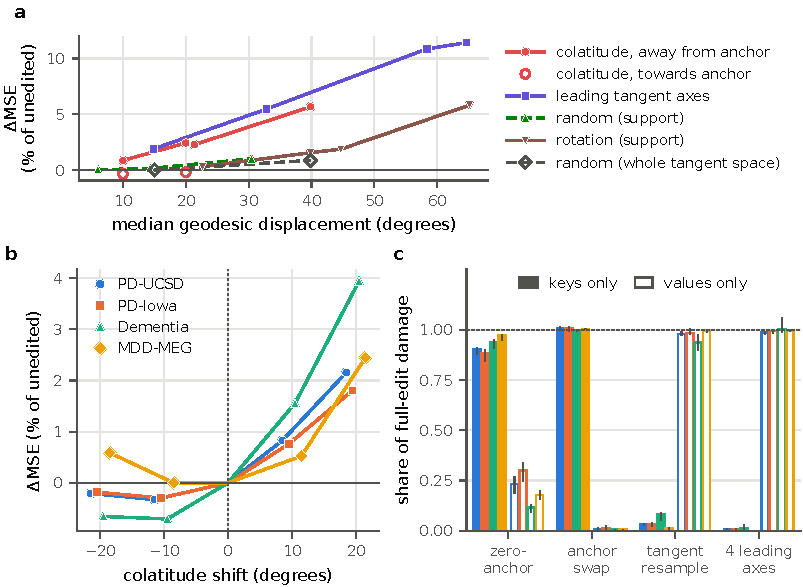
\includegraphics[width=\linewidth]{fig_interventions.pdf}
\caption{Interventions on one source at a time (released tokenizer). (a)~Change in reconstruction
  error (percent of the unedited error) against the geodesic displacement of the edited vectors, for
  families of edits (medians over sources and cohorts): colatitude shifts away from the anchor
  ($+10^\circ$, half-anchor, $+20^\circ$, zero-anchor) and towards it ($-10^\circ$, $-20^\circ$);
  resample ablation of the 1, 4, 16 and 64 leading tangent axes and of 1, 4 and 16 random directions
  of the support; rotations within the support ($30^\circ$, matched to zero-anchor, $60^\circ$,
  $90^\circ$); and the 16-dimensional resample and the matched rotation along random directions of
  the whole tangent space. (b)~Colatitude tuning (median over sources per cohort; points offset horizontally by up to
  $1.5^\circ$ for visibility); the point at
  $0^\circ$ is the unedited reconstruction. (c)~Damage of zero-anchor, the anchor swap, tangent
  resample and the resample of the four leading tangent axes when the edit enters only the decoder's
  attention keys (filled bars) or only its values (open bars), relative to the full edit (dashed
  line); medians over sources with interquartile ranges; colors denote cohorts as in (b).}
\label{fig:interventions}
\end{figure}

\subsection{The content of a source lies along its leading tangent axes}\label{sec:res-content}

Replacing the tangent direction of a source by that of another subject's vectors, while
keeping the colatitude, caused \TangentOverSourceMedianPct\% of the damage of replacing the
whole source, so the tangent direction carries the content of the source in the segment. This
content was concentrated along the leading tangent axes (\cref{fig:interventions}a). Resampling
the components on the 1, 4, 16 and 64 leading axes reproduced \ShareTPConeMedianPct,
\ShareTPCfourMedianPct, \ShareTPCsixteenMedianPct{} and \ShareTPCsixtyfourMedianPct\% of the
damage of resampling the whole tangent direction, against \ShareRandoneMedianPct,
\ShareRandfourMedianPct{} and \ShareRandsixteenMedianPct\% for 1, 4 and 16 random directions of
the support (the leading axes were more damaging for all \SourceCohortPairs{} pairs in each of the
three comparisons\GuardTPCAll) and \ShareRandOffMedianPct\% for 16
random directions of the whole tangent space. The 16 leading axes hold
\TangentSixteenMin--\TangentSixteenMax\% of the variance of the tangent direction, and resampling
them moved the vectors further than resampling 16 random directions of the support (median
displacement \DispTPCsixteen$^\circ$ against \DispRandsixteen$^\circ$). The difference is
nevertheless not one of displacement: resampling the four leading axes moved the vectors about as
far as resampling 16 random support directions (\DispTPCfour$^\circ$) and still reproduced
\ShareTPCfourMedianPct\% of the tangent damage, and at displacements up to about $40^\circ$, edits
along the leading axes were several times more damaging than edits along random directions of the
support, and in the pooled medians at least as damaging as moving the vectors away from the anchor
by a similar angle (\cref{fig:interventions}a; in Dementia about equally or less damaging). Mean ablation of
the leading axis and of the four leading axes reproduced \ShareTPCMeanOneMedianPct\% and
\ShareTPCMeanFourMedianPct\% of the tangent damage, and collapsing all vectors onto the anchor,
which removes all content but also moves the vectors to colatitude zero, caused \PoleOverSourcePct\% of
the damage of replacing the source.

\subsection{Location and identity are read through the decoder's keys, content through its values}\label{sec:res-routing}

The decoder can tell the sources apart only through their quantized vectors
(\cref{sec:background}), which suggests that the anchors act as addresses through which the
sensors' attention finds each source. Splitting the edits between the two pathways of the
decoder's attention supports this (\cref{fig:interventions}c). Applied only to the input of the
keys, with the values computed from the unedited vectors, zero-anchor reproduced a median of
\KeysZeroMedianPct\% of its full damage (cohort medians \KeysZeroCohortMin--\KeysZeroCohortMax\%);
applied only to the values, it reproduced \ValuesZeroMedianPct\% (the two shares need not add up
to 100\%; keys more damaging than values for \KeysOverValuesZeroCount{} of \SourceCohortPairs{}
pairs). Moving a source to its equator reduced the mean attention that the sensors paid to it by
a median of \AttnDropMedianPct\% (by up to \AttnDropMax\%; an interval below zero for
\AttnDecreasedCount{} of \SourceCohortPairs{} pairs), leaving it \AttnUniformMin--\AttnUniformMax\%
of the attention that a uniform allocation would give. Rotating all vectors of a source so that its
anchor coincided with that of another source, which preserves every angle within the source,
caused \SwapOverSourceMedianPct\% of the damage of replacing the source by another subject's
vectors, and this damage arose almost entirely through the keys (keys only: \KeysSwapMedianPct\%;
values only: \ValuesSwapMedianPct\% of the damage of the swap to the same partner). Content edits showed the opposite
pattern: resampling the whole tangent direction reproduced \ValuesTangentMedianPct\% of its
damage through the values and \KeysTangentMedianPct\% through the keys (values more damaging
for \ValuesOverKeysTangentCount{} of \RoutingPairs{} pairs), and resampling the four leading
tangent axes \ValuesTPCfourMedianPct\% and \KeysTPCfourMedianPct\%. Each source therefore carries
a two-part code: where its vectors lie relative to the anchors determines, through the keys, how
much the sensors read from it, and the positions of its vectors along a few leading tangent axes
determine, through the values, what they read.

\subsection{Tokens: the first level carries the source's identity}\label{sec:res-tokens}

Source identity is concentrated in the first token level (\cref{tab:tokens}; ranges over
cohorts). The level-1 code carried \MILevelOneMin--\MILevelOneMax{} of the 4~bits of source
identity (\MIShareLevelOneMin--\MIShareLevelOneMax\%), and assigning every code to the source
that uses it most often recovered the source of \SourceAccLevelOneMin--\SourceAccLevelOneMax\%
of the vectors; the deeper levels carried at most \MIDeepMax{}~bits. Identity is nevertheless
only part of what the first token encodes: it accounted for
\MIShareCodeLevelOneMin--\MIShareCodeLevelOneMax\% of the entropy of the level-1 code
(\CodeEntropyLevelOneMin--\CodeEntropyLevelOneMax~bits), the rest distinguishing vectors of the
same source. Each source used a restricted set of level-1 codewords (median per-source
perplexity \PerplexLevelOneMin--\PerplexLevelOneMax{} of 512), and these codewords pointed along
its anchor (usage-weighted cosine \CodewordCosMin--\CodewordCosMax{} across sources, cohort
medians \CodewordCosMedianMin--\CodewordCosMedianMax); at levels 2--4 every
source used nearly the whole codebook (median per-source perplexity
\PerplexDeepMin--\PerplexDeepMax).

The edits changed the codes as the geometry predicts. Moving the vectors of a source to its
anchor's equator changed \FlipZeroLevelOne\% of their level-1 codes, and \ForeignZero\% of the
new codes were codes used most often by another source; a colatitude shift of $+20^\circ$
changed \FlipColatPTwentyLevelOne\% of the level-1 codes (\ForeignColatPTwenty\% of them to
another source's codes), whereas a shift of $-20^\circ$, towards the anchor, changed
\FlipColatMTwentyLevelOne\% almost without leaving the source's vocabulary (median
\ForeignColatMTwenty\%, at most \ForeignColatMTwentyMax\%).
Content edits also changed level-1 codes mostly within the source's own vocabulary: replacing
the tangent direction changed \FlipTangentLevelOne\% of them, of which \ForeignTangent\% went to
another source's codes, and among the vectors whose level-1 code was unchanged it changed the
level-2 code of \DeeperTangentLevelTwo\% (random-support resample of 16 directions:
\DeeperRandSixteenLevelTwo\%). Moving a vector away from its anchor thus moves its first token into
the vocabulary of other sources, whereas moving it towards the anchor or changing its tangent
direction selects other tokens of the same source.

\begin{table}[tbp]
\renewcommand{\baselinestretch}{1}
\caption{Token structure (released tokenizer). $I(S;C_\ell)$: mutual information between the source index and the level-$\ell$ code (bits; $H(S)=4$~bits); accuracy: identification of the source from the level-1 code; perplexity: per-source perplexity of code usage (median over sources; 512 codewords); codeword--anchor cosine: usage-weighted cosine between a source's level-1 codewords and its anchor (median over sources). Lower part: fraction of vectors whose level-1 code changes under an edit and, in parentheses, the fraction of these changes that go to a code used most often by another source (medians over sources).}
\label{tab:tokens}
\centering\footnotesize
\setlength{\tabcolsep}{3pt}
\begin{tabular}{lcccc}
\toprule
& \textbf{PD-UCSD} & \textbf{PD-Iowa} & \textbf{Dementia} & \textbf{MDD-MEG} \\
\midrule
$I(S;C_1)$ (bits) & 3.54 & 3.51 & 3.00 & 3.96 \\
$I(S;C_\ell)$, $\ell=2,3,4$ (bits) & 0.09--0.15 & 0.05--0.12 & 0.06--0.13 & 0.05--0.14 \\
source accuracy from $C_1$ & 92\% & 92\% & 82\% & 99\% \\
perplexity, level 1 & 41 & 41 & 55 & 29 \\
perplexity, levels 2--4 & 445--454 & 456--475 & 442--471 & 437--449 \\
codeword--anchor cosine & 0.82 & 0.82 & 0.78 & 0.86 \\
\midrule level-1 codes changed by &  &  &  &  \\
\quad zero-anchor & 94\% (99\%) & 93\% (99\%) & 88\% (99\%) & 96\% (98\%) \\
\quad colatitude $+20^\circ$ & 59\% (77\%) & 58\% (78\%) & 63\% (88\%) & 44\% (60\%) \\
\quad colatitude $-20^\circ$ & 46\% (0\%) & 45\% (1\%) & 48\% (4\%) & 41\% (0\%) \\
\quad mean-anchor & 18\% (18\%) & 18\% (17\%) & 24\% (34\%) & 10\% (1\%) \\
\quad tangent resample & 97\% (10\%) & 97\% (12\%) & 97\% (23\%) & 96\% (1\%) \\
\quad tangent-axis resample (16) & 96\% (8\%) & 96\% (9\%) & 97\% (21\%) & 96\% (1\%) \\
\quad random-support resample (16) & 47\% (9\%) & 47\% (10\%) & 50\% (21\%) & 46\% (1\%) \\
\quad matched rotation (support) & 59\% (5\%) & 59\% (5\%) & 53\% (14\%) & 64\% (1\%) \\
\bottomrule
\end{tabular}
\end{table}


\subsection{The embedded copy and the replicas reproduce the anchors and the identity code; the replicas
read location through both pathways}\label{sec:res-replication}

\Cref{tab:replication} and \cref{fig:replication} compare the released tokenizer with the copy
embedded in the foundation-model checkpoints and with the tokenizers trained from scratch. The
embedded tokenizer, whose encoder and decoder equal those of the released tokenizer up to rounding
but whose codebooks differ, had the same anchors (per-source cosine $\geq$\,\EmbeddedAnchorCosMin{}
in PD-UCSD and PD-Iowa) and the same token structure ($I(S;C_1)$ of
\EmbMILevelOneMin--\EmbMILevelOneMax{} bits; zero-anchor changed the level-1 code of
\EmbFlipZeroLevelOne\% of the vectors), and zero-anchor increased its reconstruction error for
\EmbZeroAnchorPositiveCount{} of the 16 sources in PD-UCSD (median \EmbZeroAnchorRel\% of the
unedited error; applied to the keys alone, \EmbKeysZeroMedianPct\% of that damage).

\begin{table}[tbp]
\renewcommand{\baselinestretch}{1}
\caption{Tokenizers compared: released (all subjects of the four cohorts); embedded, the tokenizer stored in the foundation-model checkpoints (PD-UCSD and PD-Iowa, all subjects; interventions on PD-UCSD only); replicas trained from scratch and the source-embedding variants (held-out subjects of the four cohorts). Ranges over cohorts. MSE: median over all segments of the reconstruction error of a segment on all sensors (the released tokenizer reached 0.37--0.39 on the subjects of the embedded tokenizer and \RepReleasedMSEMin--\RepReleasedMSEMax{} on the held-out subjects of the tokenizers trained from scratch); $\Rbar$: range over sources and cohorts; anchor dim.: effective number of directions spanned by the 16 anchors (participation ratio of their cosine matrix); zero-anchor: median $\dmse$ in percent of the unedited error and number of source--cohort pairs with an interval above zero, out of all pairs evaluated; keys, values: damage of zero-anchor applied to the decoder's keys alone or to its values alone, relative to the damage of the full edit; $I(S;C_1)$: bits.}
\label{tab:replication}
\centering\scriptsize
\setlength{\tabcolsep}{2pt}
\begin{tabular}{lccccccc}
\toprule
\textbf{tokenizer} & \textbf{MSE} & $\Rbar$ & \textbf{anchor dim.} & \textbf{zero-anchor} & \textbf{keys} & \textbf{values} & $I(S;C_1)$ \\
\midrule
released & 0.31--0.39 & 0.49--0.73 & 3.9--4.0 & 3.9--8.1\% (64/64) & 0.88--0.97 & 0.12--0.30 & 3.00--3.96 \\
embedded & 0.38--0.40 & 0.57--0.73 & 4.0 & 4.6\% (16/16) & 0.89 & 0.23 & 3.46--3.51 \\
replica 1 & 0.45--0.58 & 0.92--0.97 & 2.0 & 1.6--2.7\% (64/64) & 0.79--1.31 & 1.82--2.48 & 3.61--3.91 \\
replica 2 & 0.45--0.55 & 0.91--0.97 & 2.0 & 1.4--3.0\% (64/64) & 0.51--0.70 & 1.10--2.40 & 3.60--3.78 \\
variant 1 & 0.31--0.43 & 0.87--0.95 & 1.0 & 4.5--10.8\% (64/64) & 0.00 & 1.04--1.08 & 0.06--0.17 \\
variant 2 & 0.36--0.48 & 0.91--0.97 & 1.0 & 5.1--9.7\% (64/64) & 0.01--0.02 & 1.26--1.45 & 0.34--0.79 \\
\bottomrule
\end{tabular}
\end{table}


\begin{figure}[tbp]
\centering
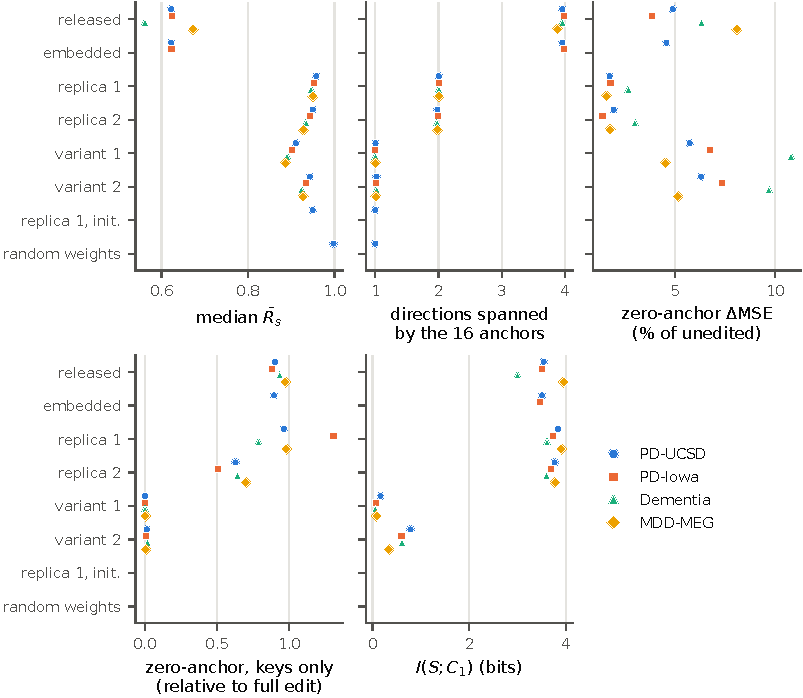
\includegraphics[width=\linewidth]{fig_replication.pdf}
\caption{Key quantities for every tokenizer examined (rows) and cohort (colors and markers):
median mean resultant length of the sources; number of directions spanned by the 16 anchors
(participation ratio of their cosine matrix); median damage of zero-anchor in percent of the
unedited error; median damage of zero-anchor applied to the decoder's keys alone, relative to the
full edit; and
$I(S;C_1)$. The tokenizers trained from scratch were evaluated on held-out subjects; the
untrained controls (initialization of replica~1; released architecture with random weights) are
shown for the geometry only (embedded: PD-UCSD and PD-Iowa, interventions on PD-UCSD only; untrained
controls: PD-UCSD).}
\label{fig:replication}
\end{figure}

The replicas reconstructed the held-out subjects less accurately than the released tokenizer
(median error of a segment \RepMSEMin--\RepMSEMax, against \RepReleasedMSEMin--\RepReleasedMSEMax{}
for the released tokenizer on the same subjects), as expected from their much smaller training
(\cref{sec:methods-replicas}). Their sources nevertheless developed the structure described above,
starting from an initialization at which all sources coincided (\cref{sec:res-geometry}). In every
replica and cohort, the vectors of each source were concentrated in a narrow cap around their anchor
(in replica~2 the anchors of two sources nearly coincided; see below), and the anchors estimated on
different cohorts agreed (per-source cosine $\geq$\,\RepCrossCohortMin; all four cohorts contributed
training data, so this agreement is expected). The anchor was the leading
uncentered direction (cosine $\geq$\,\RepCosUncMin) but carried only
\RepAnchorVarFracMin--\RepAnchorVarFracMax\% of the centered variance, about as much as the
\RepAnchorRankMin- to \RepAnchorRankMax-ranked centered PC (absolute cosine with the first centered PC
at most \RepCosCPConeMax). Three features of the geometry differed from the released tokenizer. The
caps were narrower ($\Rbar_s$ between \RepRbarMin{} and \RepRbarMax; mean colatitude
\RepAngleMin--\RepAngleMax$^\circ$). The anchors were arranged on a circle rather than in four
dimensions: in every replica and cohort, two directions held at least \RepAnchorTwoShareMin\% of
the squared norm of the 16 anchors. In replica~1, consecutive anchors along the circle were
\ReplicaOneGapMin--\ReplicaOneGapMax$^\circ$ apart, close to the $22.5^\circ$ of an even spacing; in
replica~2, the anchors of two sources nearly coincided (\ReplicaTwoMinAngleMin$^\circ$ apart in every
cohort), so that its 16 sources occupied 15 positions on the circle (largest gap
\ReplicaTwoGapMax$^\circ$). And
the anchor was closer to a single centered PC, ranked \RepBestCPCRankMin{} to \RepBestCPCRankMax{}
(median absolute cosine \RepBestCPCMedian), consistent with the argument after \cref{prop:anchor}:
fewer centered eigenvalues lay near $\operatorname{Var}(a)$ (per cohort, a median of
\RepWindowCountMin--\RepWindowCountMax{} within $\lVert\bm{\gamma}_s\rVert$ of it, against
\WindowCountMin--\WindowCountMax{} in the released tokenizer), whereas $\lVert\bm{\gamma}_s\rVert$
relative to $\operatorname{Var}(a)$ was similar (median \RepGammaOverVarMedian{} against
\GammaOverVarMedian).

The causal roles replicated in part. Zero-anchor increased the reconstruction error for
\RepZeroAnchorPositiveCount{} of the \RepSourceCohortPairs{} source--cohort pairs of the two replicas
(median \RepZeroAnchorRelMin--\RepZeroAnchorRelMax\% of the unedited error across cohorts and
replicas), rotating a source onto another source's anchor acted through the keys
(\RepKeysSwapMedianPct\% of the damage) rather than the values (\RepValuesSwapMedianPct\%), and the
content again lay along the leading tangent axes: resampling 16 of them reproduced
\RepShareTPCsixteenMedianPct\% of the damage of tangent resample, resampling 16 random directions of
the same support \RepShareRandsixteenMedianPct\%, and content edits acted through the values
(\RepValuesTangentMedianPct\% of the damage of tangent resample) rather than the keys
(\RepKeysTangentMedianPct\%). The location code, however, differed. Applied to the keys alone,
zero-anchor caused a median of \RepKeysZeroMedianPct\% of the damage of the full edit, and the attention
paid to the source fell by a median of \RepAttnDropMedianPct\%; applied to the values alone, it was even
more damaging than the full edit (\RepValuesZeroMedianPct\%), so that the keys were the more damaging
pathway for only \RepKeysOverValuesZeroCount{} of the \RepSourceCohortPairs{} pairs, and the decoders of these tokenizers read the
location of a source through both pathways. In their narrow caps zero-anchor moves the vectors further
(\RepMatchedDisp$^\circ$ against \MatchedDisp$^\circ$), and the matched rotation, mostly the
$180^\circ$ fallback here, was the more damaging edit for every pair, so it is no displacement control
for these tokenizers. The exact colatitude also carried information: replacing the anchor coordinate
by its mean or by that of a permuted vector increased the error for \RepMeanAnchorPositiveCount{} and
\RepResampleAnchorPositiveCount{} pairs (\RepMeanOverZeroMedianPct\% and \RepResampleOverZeroMedianPct\%
of the zero-anchor damage), and shifts towards the anchor were damaging: a shift of $10^\circ$ increased the error for
\RepColatMTenPositiveCount{} pairs, although a median of only \RepWithinTenMedianPct\% of the vectors of a
source lie within $10^\circ$ of the anchor, and a shift of $20^\circ$ was more damaging than the same
shift away, as it moves the vectors within $20^\circ$ of the anchor (a median of
\RepWithinTwentyMedianPct\%) onto the anchor itself. The first RVQ level
again carried most of the information about source identity: $I(S;C_1)$ was
\RepMILevelOneMin--\RepMILevelOneMax{} bits (\RepMIShareCodeLevelOneMin--\RepMIShareCodeLevelOneMax\%
of the entropy of the level-1 code), and zero-anchor changed the level-1 code of
\RepFlipZeroLevelOne\% of the vectors, \RepForeignZero\% of them to a code used most often by
another source.

\subsection{With a source embedding in the decoder, the anchors do not separate}\label{sec:res-variants}

The source-embedding variants test whether the organization described above follows from the
decoder's lack of a source index. Their decoders receive a learned embedding of each source, and their
training, from the same initial weights and batches as the replicas, did not separate the sources by
location: in both variants the vectors of each source were again concentrated
($\Rbar_s$ between \VarRbarMin{} and \VarRbarMax), but around nearly one common direction. In every
cohort each anchor lay within \VarAnchorToCommonMax$^\circ$ of the mean direction of the 16 anchors, less
than the mean colatitude of any source (\VarAngleMin$^\circ$ to \VarAngleMax$^\circ$), so that the caps
of all sources overlapped; any two anchors lay within \VarAnchorPairAngleMax$^\circ$ of each other
(pairwise cosine $\geq$\,\VarOffdiagMin), whereas in the replicas they lay up to
\RepAnchorPairAngleMax$^\circ$ apart. Accordingly, rotating a source onto another source's anchor
moved its vectors by only \VarDispSwap$^\circ$ (\RepDispSwap$^\circ$ in the replicas) and caused
\VarSwapOverSourceMedianPct\% of the damage of replacing the source by another subject's vectors
(\RepSwapOverSourceMedianPct\% in the replicas), and the first token level encoded little of the
source identity ($I(S;C_1)$ of \VarMILevelOneMin--\VarMILevelOneMax{} bits,
\VarMIShareCodeLevelOneMin--\VarMIShareCodeLevelOneMax\% of the entropy of the level-1 code, against
\RepMILevelOneMin--\RepMILevelOneMax{} of the 4~bits in the replicas). Variant~2, whose anchors were
more dispersed, also encoded more identity (any two anchors within
\VariantTwoAnchorPairAngleMax$^\circ$ and \VariantTwoMILevelOneRange{} bits, against
\VariantOneAnchorPairAngleMax$^\circ$ and \VariantOneMILevelOneRange{} bits in variant~1). Moving the vectors of a source away from the common anchor still
damaged the reconstruction (zero-anchor: \VarZeroAnchorPositiveCount{} of \VarSourceCohortPairs{}
pairs, median \VarZeroAnchorRelMin--\VarZeroAnchorRelMax\% of the unedited error), but almost only
through the values: applied to the keys alone, zero-anchor caused a median of \VarKeysZeroMedianPct\% of
its damage and applied to the values alone \VarValuesZeroMedianPct\%, and the attention paid to the
edited source fell by a median of only \VarAttnDropMedianPct\%. Content edits likewise acted through
the values (tangent resample: \VarValuesTangentMedianPct\% of its damage through the values,
\VarKeysTangentMedianPct\% through the keys), and the content again lay along the leading tangent axes
(resampling 16 of them: \VarShareTPCsixteenMedianPct\% of the damage of tangent resample; 16 random
support directions: \VarShareRandsixteenMedianPct\%). In these tokenizers the keys thus hardly respond
to the quantized vectors, and the sensors find each source through its embedding. In every cohort, each
variant reconstructed the held-out subjects better than the replica of the same seed (median error of a segment \VarMSEMin--\VarMSEMax{}
against \RepMSEMin--\RepMSEMax; released tokenizer on the same subjects
\RepReleasedMSEMin--\RepReleasedMSEMax) and fitted its training batches better (correlation between
reconstructed and target waveforms at the end of training \VarPCCRange{} against \RepPCCRange).

\subsection{Diagnostic information is present in the sources but, within cohorts, not concentrated in the anchors}\label{sec:res-diagnosis}

\Cref{tab:readout} and \cref{fig:readout} summarize the subject-level read-outs. In the three
contrasts in which band power distinguished patients from controls---Alzheimer's disease (AD; AUC
\BandADAUC), frontotemporal dementia (FTD; \BandFTDAUC) and Parkinson's disease at the Iowa site
(\BandIowaPDAUC)---the full source representation and the per-source means of the quantized vectors
did so as well (full \FullADAUC, \FullFTDAUC{} and \FullIowaPDAUC; quantized \QuantADAUC,
\QuantFTDAUC{} and \QuantIowaPDAUC; all significant after correction). In AD and PD-Iowa their AUCs
were close to those of band power (paired difference of the full representation
\PairedFullBandAD{} \PairedFullBandADCI{} and \PairedFullBandIowaPD{} \PairedFullBandIowaPDCI), whereas
in FTD their point estimates were lower (full \PairedFullBandFTD{} \PairedFullBandFTDCI; quantized
\PairedQuantBandFTD{} \PairedQuantBandFTDCI; descriptive intervals with the out-of-fold scores held
fixed, \cref{sec:methods-readout}), a difference these data do not establish. The tokenizer thus retains much of the diagnostic information that band power captures,
with a possible loss in FTD. In PD-UCSD (\NUCSDPD{} subjects) and MDD-MEG (\NMDD{} subjects), no representation
separated the groups, band power included. Age and sex alone separated the groups at most weakly
(AUC \AgeSexADAUC{} in AD, \AgeSexFTDAUC{} in FTD and \AgeSexIowaPDAUC{} in PD-Iowa,
\AgeSexIowaPDP{} uncorrected; \AgeSexMDDAUC{} in MDD-MEG, \AgeSexMDDP{} uncorrected), and regressing
them out of the features inside every training fold left the full representation and band power
above chance (full: \FullAdjADAUC, \FullAdjFTDAUC{} and \FullAdjIowaPDAUC; band power:
\BandAdjADAUC, \BandAdjFTDAUC{} and \BandAdjIowaPDAUC). In PD-UCSD, where age and sex are matched
between the groups, the classifier on age and sex alone was below chance (\AgeSexUCSDPDAUC), as can
occur in cross-validation when covariates are more closely matched between the groups than random
labels would make them \citep{parker2007stratification,airola2011auc}; its permutation statistic lay
in the lower tail of the null distribution of the same pipeline (null mean \AgeSexUCSDPDNullMean,
\AgeSexUCSDPDP), so the test was not misled.

\begin{sidewaystable}
\renewcommand{\baselinestretch}{1}
\caption{Subject-level diagnostic read-out (released tokenizer): AUC (mean over 20 repetitions of stratified five-fold cross-validation) with a 95\% stratified bootstrap interval over subjects in which the out-of-fold scores are held fixed (it does not include the variability of model fitting; inference rests on the permutation tests). Markers: $^{*}$ permutation $p<0.05$ (anchor-16: Holm-corrected across contrasts; secondary representations: Benjamini--Hochberg-corrected within contrast; best single anchor, adjusted representations and age and sex: uncorrected). The permutation tests use the pipeline with the inverse regularization strength fixed at 1 and two repetitions (\cref{sec:methods-readout}), whose statistic differs from the AUC shown by at most \PermStatMaxDiff, so a marked AUC can have an interval that includes 0.5. Best single anchor: the anchor coordinate whose AUC on the training subjects is farthest from 0.5, selected inside every training fold and evaluated out of fold (per-source results are given in the text); adjusted: age and sex regressed out within training folds. Last row: AUC range (2.5--97.5\% quantiles) of 100 random 16-direction representations evaluated like anchor-16.}
\label{tab:readout}
\centering\scriptsize
\setlength{\tabcolsep}{2pt}
\begin{tabular}{lccccc}
\toprule
& \textbf{PD-UCSD} & \textbf{PD-Iowa} & \textbf{Dementia} & \textbf{Dementia} & \textbf{MDD-MEG} \\
& \textbf{PD vs HC} ($n=31$) & \textbf{PD vs HC} ($n=148$) & \textbf{AD vs CN} ($n=65$) & \textbf{FTD vs CN} ($n=52$) & \textbf{MDD vs HV} ($n=49$) \\
\midrule
anchor-16 & 0.62 [0.48, 0.76] & 0.67$^{*}$ [0.59, 0.75] & 0.72$^{*}$ [0.61, 0.82] & 0.65 [0.52, 0.77] & 0.42 [0.31, 0.55] \\
best single anchor & 0.44 [0.31, 0.57] & 0.59 [0.51, 0.67] & 0.67$^{*}$ [0.57, 0.78] & 0.70$^{*}$ [0.56, 0.83] & 0.47 [0.36, 0.59] \\
quantized anchor-16 & 0.53 [0.38, 0.67] & 0.70$^{*}$ [0.61, 0.78] & 0.75$^{*}$ [0.64, 0.85] & 0.63$^{*}$ [0.49, 0.75] & 0.49 [0.36, 0.62] \\
concentration-16 & 0.59 [0.44, 0.73] & 0.69$^{*}$ [0.61, 0.77] & 0.68$^{*}$ [0.57, 0.79] & 0.65$^{*}$ [0.52, 0.77] & 0.42 [0.31, 0.55] \\
norm-16 & 0.63 [0.50, 0.76] & 0.64$^{*}$ [0.56, 0.72] & 0.79$^{*}$ [0.68, 0.89] & 0.71$^{*}$ [0.58, 0.83] & 0.42 [0.30, 0.55] \\
pooled & 0.56 [0.40, 0.73] & 0.68$^{*}$ [0.61, 0.76] & 0.83$^{*}$ [0.73, 0.91] & 0.62$^{*}$ [0.50, 0.74] & 0.50 [0.38, 0.62] \\
tangent & 0.49 [0.33, 0.65] & 0.73$^{*}$ [0.66, 0.80] & 0.83$^{*}$ [0.72, 0.91] & 0.77$^{*}$ [0.65, 0.88] & 0.53 [0.39, 0.66] \\
full & 0.52 [0.35, 0.68] & 0.73$^{*}$ [0.66, 0.80] & 0.83$^{*}$ [0.73, 0.91] & 0.76$^{*}$ [0.64, 0.87] & 0.52 [0.39, 0.65] \\
quantized & 0.48 [0.32, 0.65] & 0.71$^{*}$ [0.63, 0.79] & 0.82$^{*}$ [0.72, 0.91] & 0.75$^{*}$ [0.63, 0.86] & 0.54 [0.40, 0.67] \\
band power & 0.52 [0.39, 0.66] & 0.73$^{*}$ [0.65, 0.80] & 0.83$^{*}$ [0.74, 0.91] & 0.83$^{*}$ [0.73, 0.93] & 0.49 [0.35, 0.62] \\
anchor-16, adjusted & 0.63 [0.50, 0.77] & 0.68$^{*}$ [0.60, 0.76] & 0.70$^{*}$ [0.59, 0.81] & 0.62$^{*}$ [0.50, 0.73] & 0.50 [0.38, 0.62] \\
full, adjusted & 0.52 [0.35, 0.69] & 0.73$^{*}$ [0.64, 0.80] & 0.79$^{*}$ [0.68, 0.89] & 0.78$^{*}$ [0.66, 0.89] & 0.50 [0.38, 0.62] \\
band power, adjusted & 0.49 [0.37, 0.62] & 0.72$^{*}$ [0.63, 0.79] & 0.81$^{*}$ [0.71, 0.90] & 0.83$^{*}$ [0.71, 0.92] & 0.53 [0.40, 0.66] \\
age and sex & 0.31 [0.26, 0.35] & 0.58$^{*}$ [0.51, 0.65] & 0.57 [0.48, 0.67] & 0.54 [0.43, 0.66] & 0.64$^{*}$ [0.52, 0.76] \\
\midrule random 16 directions & 0.38--0.66 & 0.56--0.74 & 0.66--0.86 & 0.53--0.81 & 0.37--0.62 \\
\bottomrule
\end{tabular}
\end{sidewaystable}


\begin{figure}[tbp]
\centering
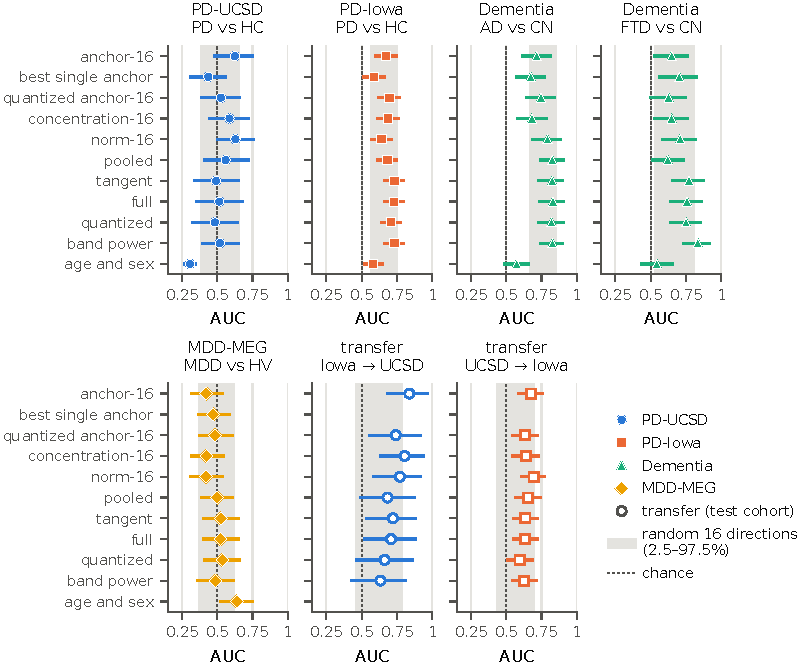
\includegraphics[width=\linewidth]{fig_readout.pdf}
\caption{Subject-level diagnostic read-out (released tokenizer): AUC with 95\% bootstrap interval
  (within-cohort panels: mean over 20 repetitions of stratified five-fold cross-validation, out-of-fold
  scores held fixed in the bootstrap; transfer panels: AUC of a single classifier on the test cohort,
  bootstrap over test subjects); colors denote cohorts. The last two panels (bottom row; open
  markers, colored by the cohort tested) show transfer between the Parkinson's cohorts: a classifier
  trained on all subjects of one cohort and tested on the other, with the training cohort's feature
  scaling; band power is restricted to the shared sensors; rows without a value (best single anchor,
  age and sex) were not evaluated for transfer. The grey band is the 2.5--97.5\% range of the AUCs of
  random 16-direction representations evaluated like anchor-16 (100 draws within cohorts,
  \TransferIowaToUCSDRandN{} in the transfer panels); the dashed line marks chance.}
\label{fig:readout}
\end{figure}

The anchor coordinates carried less of this information. Anchor-16 was above chance after Holm
correction across the \NumContrasts{} contrasts in \AnchorSignificantCount{} of them (AD:
\AnchorADAUC{} \AnchorADCI, \AnchorADPHolm; PD-Iowa: \AnchorIowaPDAUC{} \AnchorIowaPDCI,
\AnchorIowaPDPHolm) but not in FTD (\AnchorFTDAUC{} \AnchorFTDCI, \AnchorFTDPHolm). In all three
its AUC was below that of the full representation (paired difference full minus anchor-16:
\PairedFullAnchorAD{} \PairedFullAnchorADCI{} in AD, \PairedFullAnchorIowaPD{}
\PairedFullAnchorIowaPDCI{} in PD-Iowa and \PairedFullAnchorFTD{} \PairedFullAnchorFTDCI{} in FTD),
and 16 random directions of the same per-source representation, evaluated identically, reached at
least the same AUC in \RandADGePct\%, \RandIowaPDGePct\% and \RandFTDGePct\% of 100 draws
(\RandUCSDPDGePct\% in PD-UCSD and \RandMDDGePct\% in MDD-MEG; Monte Carlo $p\geq\RandMCPMin$ in every
contrast). Within cohorts, the anchors are therefore not a privileged summary of the diagnostic
information. Individually, the
anchor coordinate of source \SingleADBestSource{} separated patients from controls after
family-wise correction across the 16 sources of each contrast in both AD (AUC \SingleADBestAUC,
\SingleADMinP) and FTD (\SingleFTDBestAUC, \SingleFTDMinP), which share their control group; in
total, \SingleADSigCount{} sources did so in AD, \SingleFTDSigCount{} in FTD and
\SingleIowaPDSigCount{} in PD-Iowa (source \SingleIowaPDBestSource, \SingleIowaPDBestAUC,
\SingleIowaPDMinP), and none in PD-UCSD or MDD-MEG. Selecting the best source inside every training
fold, which accounts for the selection, gave AUCs of \BestSingleADAUC{} in AD and \BestSingleFTDAUC{}
in FTD (\cref{tab:readout}).

\begin{table}[tbp]
\renewcommand{\baselinestretch}{1}
\caption{Transfer between the two Parkinson's cohorts (released tokenizer): a classifier trained on all subjects of one cohort and applied to the other. AUC with 95\% bootstrap interval over the test subjects; $p$: permutation of the test labels, Holm-corrected across the two directions for anchor-16 and Benjamini--Hochberg-corrected within a direction for the other representations; rand.: number of the 1{,}000 random 16-direction representations with at least the same AUC. Band power is restricted to the 29 sensors shared by the two montages.}
\label{tab:transfer}
\centering\scriptsize
\setlength{\tabcolsep}{4pt}
\begin{tabular}{lcccccc}
\toprule
& \multicolumn{3}{c}{PD-Iowa $\to$ PD-UCSD} & \multicolumn{3}{c}{PD-UCSD $\to$ PD-Iowa} \\
\cmidrule(lr){2-4}\cmidrule(lr){5-7}
\textbf{representation} & AUC & $p$ & rand. & AUC & $p$ & rand. \\
\midrule
\multicolumn{7}{@{}l}{\emph{features standardized with the training cohort's statistics}} \\
anchor-16 & 0.84 [0.68, 0.97] & $<$0.001 & 2 & 0.68 [0.58, 0.76] & $<$0.001 & 62 \\
quantized anchor-16 & 0.74 [0.55, 0.93] & 0.030 & 88 & 0.63 [0.53, 0.73] & 0.006 & 202 \\
concentration-16 & 0.80 [0.63, 0.94] & 0.017 & 13 & 0.64 [0.54, 0.73] & 0.006 & 188 \\
norm-16 & 0.77 [0.58, 0.93] & 0.020 & 48 & 0.69 [0.60, 0.78] & $<$0.001 & 28 \\
pooled & 0.68 [0.48, 0.88] & 0.057 & 252 & 0.65 [0.56, 0.75] & 0.006 & 128 \\
tangent & 0.72 [0.53, 0.89] & 0.043 & 131 & 0.64 [0.55, 0.73] & 0.006 & 197 \\
full & 0.71 [0.51, 0.89] & 0.043 & 158 & 0.63 [0.55, 0.73] & 0.006 & 203 \\
quantized & 0.66 [0.46, 0.87] & 0.077 & 342 & 0.60 [0.50, 0.69] & 0.030 & 417 \\
band power & 0.63 [0.42, 0.82] & 0.110 & 492 & 0.63 [0.54, 0.72] & 0.007 & 244 \\
\midrule
\multicolumn{7}{@{}l}{\emph{features standardized within each cohort}} \\
anchor-16 & 0.81 [0.64, 0.95] & 0.002 & 13 & 0.71 [0.62, 0.80] & $<$0.001 & 16 \\
quantized anchor-16 & 0.74 [0.55, 0.91] & 0.035 & 82 & 0.70 [0.60, 0.79] & $<$0.001 & 28 \\
concentration-16 & 0.77 [0.58, 0.92] & 0.019 & 40 & 0.64 [0.54, 0.74] & 0.005 & 202 \\
norm-16 & 0.78 [0.58, 0.93] & 0.019 & 30 & 0.69 [0.60, 0.78] & $<$0.001 & 39 \\
pooled & 0.58 [0.38, 0.80] & 0.229 & 702 & 0.66 [0.57, 0.76] & 0.003 & 115 \\
tangent & 0.70 [0.50, 0.89] & 0.053 & 185 & 0.64 [0.55, 0.73] & 0.005 & 229 \\
full & 0.71 [0.52, 0.89] & 0.049 & 141 & 0.64 [0.55, 0.74] & 0.005 & 192 \\
quantized & 0.64 [0.43, 0.85] & 0.112 & 408 & 0.60 [0.51, 0.70] & 0.022 & 393 \\
band power & 0.66 [0.46, 0.85] & 0.099 & 340 & 0.62 [0.53, 0.72] & 0.008 & 291 \\
\bottomrule
\end{tabular}
\end{table}


Across sites (\cref{tab:transfer}), the representations transferred above chance in most cases,
and the anchor coordinates stood out against random directions in one of the two directions with the
training cohort's feature scaling and in both with features standardized within each cohort. A
classifier trained on all PD-Iowa subjects and applied to PD-UCSD, recorded at another site with
another montage, reached an AUC of \TransferIowaToUCSDAnchorAUC{} \TransferIowaToUCSDAnchorCI{} with
the anchor coordinates (\TransferIowaToUCSDAnchorP), higher than all but
\TransferIowaToUCSDRandGeCount{} of \TransferIowaToUCSDRandN{} representations by 16 random directions
(Monte Carlo \TransferIowaToUCSDRandP{}, Holm-corrected across the two directions; 2.5--97.5\% range
\TransferIowaToUCSDRandRange); trained on the \NUCSDPD{} PD-UCSD subjects and applied to PD-Iowa, the
anchor coordinates reached \TransferUCSDToIowaAnchorAUC{} \TransferUCSDToIowaAnchorCI{}
(\TransferUCSDToIowaAnchorP), in the upper tail of the random directions
(\TransferUCSDToIowaRandGeCount{} of \TransferUCSDToIowaRandN{} at least as high; Monte Carlo
\TransferUCSDToIowaRandP). With the features standardized within each cohort, the anchor coordinates
reached \TransferIowaToUCSDHarmAnchorAUC{} and \TransferUCSDToIowaHarmAnchorAUC, above the random
directions in both directions (Monte Carlo \TransferIowaToUCSDHarmRandP{} and
\TransferUCSDToIowaHarmRandP, Holm-corrected). With Holm correction across both scalings and both
directions (four tests), the Monte Carlo $p$-values are \TransferIowaToUCSDRandPHolmFour{} and
\TransferUCSDToIowaRandPHolmFour{} with the training cohort's scaling and
\TransferIowaToUCSDHarmRandPHolmFour{} and \TransferUCSDToIowaHarmRandPHolmFour{} with the features
standardized within each cohort, so each conclusion is unchanged\GuardHolmFour. With one exception (below), the anchor coordinates were
nevertheless not shown to transfer better than the other representations, all of which also
transferred from PD-UCSD to PD-Iowa (largest corrected \TransferUCSDToIowaMaxSecondaryP{} with the
training cohort's scaling and \TransferUCSDToIowaHarmMaxSecondaryP{} with the features standardized
within each cohort) and some of which transferred from PD-Iowa to PD-UCSD.
With the training cohort's feature scaling no paired difference between the anchor coordinates and
another representation was significant after correction, the largest being those to band power
(\TransferIowaToUCSDAnchorMinusBand, unadjusted interval \TransferIowaToUCSDAnchorMinusBandCI,
Holm-corrected \TransferIowaToUCSDAnchorMinusBandP) and to the quantized representation
(\TransferIowaToUCSDAnchorMinusQuant, \TransferIowaToUCSDAnchorMinusQuantCI,
\TransferIowaToUCSDAnchorMinusQuantP) from PD-Iowa to PD-UCSD; with the features standardized within
each cohort, the only significant one was that to concentration-16 from PD-UCSD to PD-Iowa
(\TransferUCSDToIowaHarmAnchorMinusRbar, \TransferUCSDToIowaHarmAnchorMinusRbarCI, Holm-corrected
\TransferUCSDToIowaHarmAnchorMinusRbarP). The other per-source scalar summaries, concentration-16 and
norm-16, transferred in both directions and lay in the upper tail of the random directions from
PD-Iowa to PD-UCSD, norm-16 also from PD-UCSD to PD-Iowa (\cref{tab:transfer}).

%% =========================================================================
\FloatBarrier
\section{Discussion}\label{sec:discussion}

\subsection{Anchors as addresses, tangent axes as content}

The latent sources of BrainOmni's tokenizer are not interchangeable channels with arbitrary
content. Each source occupies a cap around its own learned anchor, which is nearly the same for
every montage, site, population and modality we examined; the caps overlap (the smallest angle
between two anchors is below the mean colatitude), and the vectors of a source carry a two-part
code. The location of the vectors relative to the anchors determines, through the decoder's
attention keys, how much the sensors read from a source: vectors moved towards the equator receive
less attention, and rotating them onto another source's anchor damages the reconstruction almost
entirely through the keys, consistent with their being read as if they came from another source.
The content lies in the tangent direction, concentrated along a few leading tangent axes, and
reaches the reconstruction through the attention values; the exact colatitude carries little of
it. The anchor direction is thus an address rather than a carrier of content: it resembles the
constant offsets and outlier directions that act as biases in language and vision transformers
\citep{bis2021toomuch,timkey2021rogue,sun2024massive,darcet2024registers}, except that its role is
to keep the sources apart. These addresses occupy few of the 256 dimensions: the 16 anchors lie close to a
four-dimensional subspace in the released tokenizer and close to a circle in the replicas we
trained (\cref{sec:res-replication}).

The architecture suggests why such a code arises. Every source is an attention-weighted
average of the same per-sensor features passed through shared value and output projections, the
quantizer discards its norm and uses codebooks shared by all sources, and the decoder receives
neither a source index nor a source embedding. The quantized vectors themselves are therefore the
only channel through which the decoder can learn which source a vector belongs to. With the
released initialization all sources point in the same direction; the released training separated
them (at our much smaller training scale the sources did not separate in a pilot run with this
initialization, which we therefore modified; \cref{sec:methods-replicas}), and the
first RVQ level then carries most of the information about source identity, although identity is
less than half of what a level-1 token encodes. The source-embedding variants support this account
(\cref{sec:res-variants}): when the decoder could identify the sources through a learned embedding,
training from the replicas' initial weights and batches left all sources around nearly one common
direction (so the modified initialization does not by itself separate them), the first token level encoded little
source identity, and the keys hardly responded to the quantized vectors. Separated anchors, the reading of identity
through the keys and the identity code of the first token level thus appear as three consequences of
one constraint, that the quantized vectors are the decoder's only access to source identity; the
evidence comes from two variants, each paired with a replica of the same seed, trained at a small
scale. For BrainOmni's foundation
model this identity information is redundant: the model adds the encoder's learned query vector
of each source to that source's tokens. Subtracting the learned anchors before quantization or
giving each source its own first-level codebook are natural ways to reclaim the capacity; whether
they improve downstream performance is a question for future work.

\subsection{Implications for interpreting representations}

\Cref{tab:standard} sets what three standard analyses suggest about the anchors of the released
tokenizer against what the analyses used here show. Four methodological points generalize beyond
this model. First, for a representation concentrated
around a mean direction, the leading eigenvector of the uncentered second moment lies close to that
direction whenever the cross-covariance between the coordinate along it and the orthogonal part is
small compared with the gap between the mean squared coordinate and the second eigenvalue
(\cref{prop:anchor}); a coordinate that varies little guarantees this. The centered principal
components instead describe the variation around the mean direction
\citep{mu2018allbutthetop,honeine2014centering}. Statements that a mean direction ``is the top
principal component'', and control directions chosen by principal-component rank, must therefore
name the second moment they refer to. Second,
edits of normalized representations should preserve the normalization: some edits that move
vectors off the sphere, such as scaling or averaging the coordinate along a direction, are partly
undone when the model renormalizes them, so that the effect attributed to the edit is smaller than,
and not proportional to, the edit itself (halving the anchor component off the sphere would have
achieved \OffSphereHalfMin--\OffSphereHalfMax\% of the intended change in the released tokenizer
and only \RepOffSphereHalfMin--\RepOffSphereHalfMax\% in the narrow caps of the replicas). Third, projection (zero) ablation of a mean direction
removes a location as well as any information carried along it. Mean and resample ablation
separate the two \citep{chan2022causalscrubbing,heimersheim2024patching,zhang2024bestpractices,
li2024optimalablation}, and on the sphere, controls must also be matched in displacement and in
support, because the same displacement is nearly harmless along some directions and damaging along
others. In our data, zero ablation alone would attribute about half of the effect of replacing a
source (\ZeroOverSourceMedianPct\%) to a single direction; mean and resample ablation show that this direction carries little information,
displacement- and support-matched controls identify the directions that do, and the decomposition
of the decoder's attention into keys and values \citep{elhage2021framework} shows why the location
matters. Fourth, diagnostic read-outs from foundation-model representations of small cohorts must
be evaluated at the level of subjects with calibrated null distributions: cross-validated
estimates of the AUC are biased downwards and can fall below 0.5 when there is no signal, most
strongly for pooled leave-one-out estimates \citep{parker2007stratification,airola2011auc}, which is
why inference should rest on permutation nulls that re-run the same pipeline; segment-level splits measure subject identity
\citep{saeb2017usecase,lin2026identitytrap}; and a candidate summary should be compared with
random summaries of the same dimension.

\begin{table}[tbp]
\renewcommand{\baselinestretch}{1}
\caption{Three standard analyses of the anchors of the released tokenizer, what they suggest, and what
  the analyses used here show.}
\label{tab:standard}
\centering\footnotesize
\setlength{\tabcolsep}{3pt}
\begin{tabular}{@{}>{\raggedright\arraybackslash}p{0.17\linewidth}>{\raggedright\arraybackslash}p{0.37\linewidth}>{\raggedright\arraybackslash}p{0.42\linewidth}@{}}
\toprule
\textbf{question} & \textbf{standard analysis and what it suggests} & \textbf{analysis used here and what it shows} \\
\midrule
Is the anchor a principal direction? & Centered PCA: the anchor carries \AnchorVarFracMin--\AnchorVarFracMax\% of
  the variance of a source (ranked \AnchorRankMin{} to \AnchorRankMax), a minor direction. & Uncentered second moment
  and \cref{prop:anchor}: the anchor is the leading direction of every source (cosine $\geq$\,\CosUncMin) and
  fixes where its vectors lie (\cref{sec:res-pca}). \\
Is information carried along the anchor? & Projection (zero) ablation of the anchor: \ZeroOverSourceMedianPct\%
  of the damage of replacing the source by another subject's vectors, as if half of the information of a source
  lay along one direction. & Mean and resample ablation of the anchor coordinate: \MeanOverZeroMedianPct\% and
  \ResampleOverZeroMedianPct\% of the zero-anchor damage; zero-anchor is
  \LatitudeRatioMin--\LatitudeRatioMax{} times as damaging as rotations matched in displacement; the damage is a change of location, read
  through the decoder's keys (\KeysZeroMedianPct\%; \cref{sec:res-necessity,sec:res-routing}). \\
Are the anchor coordinates a privileged diagnostic summary within a cohort? & Linear probe tested against
  chance: above chance in \AnchorSignificantCount{} of \NumContrasts{} contrasts (AD and PD-Iowa), as if the
  anchors summarized the diagnostic information. & Probe tested against random 16-direction projections of
  the same representation: within cohorts, these reach at least the same AUC in \RandADGePct\% and
  \RandIowaPDGePct\% of draws in AD and PD-Iowa (Monte Carlo $p\geq\RandMCPMin$ in every contrast); in
  transfer between the Parkinson's cohorts, the anchor coordinates exceed them in at least one direction
  (\cref{sec:res-diagnosis}). \\
\bottomrule
\end{tabular}
\end{table}

\subsection{Diagnostic content}

The read-outs separate two questions that are easily conflated. Whether the tokenizer preserves
diagnostic information is answered by the full source representation and its quantized
counterpart, which separated the groups in every contrast in which band power was informative,
with AUCs close to those of band power in AD and PD-Iowa and somewhat lower in FTD; for these
resting-state contrasts the tokenizer retains much of the diagnostic information, although a loss
in FTD cannot be excluded. Whether that information is
concentrated in the anchors is answered by comparing the 16 anchor coordinates with random
16-dimensional projections of the same representation, and the anchor coordinates did not do
significantly better.
This is consistent with their role as addresses: a subject-level shift of the colatitude of a
source changes how strongly the decoder attends to it but carries little content. The source
whose anchor coordinate separated both dementia groups from controls shows that such shifts can
nevertheless covary with disease. Across sites the picture changed: with the training cohort's feature
scaling, the anchor coordinates trained on PD-Iowa transferred to PD-UCSD better than random
projections of the same representation, whereas in the other direction they lay in the upper tail of
the random projections, and with the features standardized within each cohort they exceeded the
random projections in both directions;
the other per-source scalar summaries (concentration and norm) also transferred, and with the
training cohort's feature scaling none of their differences from the anchor coordinates, nor those of
the full representation or band power, was significant. A plausible reading is that how strongly each
source is engaged---how close its vectors lie to the anchor, how concentrated and how large they
are---is less affected by site and montage than the content of the sources or the band power of
individual sensors. Because one side of each comparison is a cohort of 31 subjects, this
observation needs confirmation in further cohorts. Neither the source representation nor
band power separated the groups in PD-UCSD, the smallest cohort, or in MDD-MEG, in which age and
sex alone were weakly predictive; we draw no conclusion about these contrasts beyond the absence
of a detectable effect.

\subsection{Limitations}

The analysis concerns one tokenizer architecture. We examined the released checkpoint, the
differently quantized copy inside the foundation-model checkpoints and \NumReplicas{} tokenizers
trained from scratch, but the latter were trained with a much smaller corpus, batch and budget
than the released tokenizer and with a modified recipe (\cref{sec:methods-replicas}), and the replicas
reached a higher reconstruction error; other normalized-RVQ tokenizers may organize
their latent space differently. Our causal criterion is the tokenizer's own reconstruction; we
did not test how the anchors affect the BrainOmni foundation model that consumes the tokens or
its downstream accuracy. Edits were applied to one source at a time and to the quantizer input;
interactions between sources and edits of the encoder were not examined. One of the cohorts
(PD-UCSD) appears in the configuration of the released pretraining code and may have been part
of the tokenizer's self-supervised training data; the geometric and causal findings were the
same on the three other cohorts, and the tokenizers we trained, analyzed on held-out subjects only,
are compared in \cref{sec:res-replication,sec:res-variants}. For MEG we analyzed the first 180~s of each recording. The diagnostic analyses involve modest cohorts with
one or two diagnostic contrasts each, characterize representations rather than clinical utility, and were not
validated in independent clinical samples beyond the transfer between the two Parkinson's
cohorts. Finally, we describe where the anchors lie and how the decoder uses them, but not how
the encoder's attention produces them, which is a natural next step for a circuit-level account.

%% =========================================================================
\section{Conclusion}\label{sec:conclusion}

The 16 latent sources of BrainOmni's tokenizer form a structured code. Each source lives in a
cap around a learned anchor that is largely fixed by the tokenizer and shared across cohorts and
modalities; the anchor is the source's leading uncentered principal direction but carries only a
few percent of its centered variance, no more than a typical one of its roughly 20 effective
dimensions; the decoder's attention keys use the location of the vectors relative to the anchors
to decide how much to read from a source, and its values read the source's content from a few
leading tangent axes; and the first token level carries most of the information about which
source a vector belongs to. Two replicas trained from scratch reproduce the anchors, the reading of
identity through the keys, the content along leading tangent axes and the identity code, although they
read the location of a source through both attention pathways; two variants whose decoder receives an
embedding of each source do not separate the anchors and read almost nothing through the keys, which
supports the
decoder's lack of a source index as the origin of the code.
In subject-level read-outs, the source representation and its tokens carry diagnostic
information wherever band power does, and this information is not concentrated in the anchors
within a cohort, although the anchor coordinates transferred between the two Parkinson's cohorts
better than random directions, in one direction with the training cohort's feature scaling and in both
with features standardized within each cohort; with \NUCSDPD{} subjects in one of the two cohorts, this
needs confirmation in further cohorts. These conclusions rest on interventions that preserve the geometry
imposed by the quantizer and on controls matched in displacement, dimension and support, and
the same methodology can be applied to other models that normalize their latent vectors before
quantizing or attending to them.

\section*{Ethics statement}
This work uses only publicly available, de-identified datasets distributed under CC0
licenses through OpenNeuro, collected under the ethical approvals of the original
studies. No new data were collected. The diagnostic analyses characterize tokenizer
representations and are not intended or validated for clinical use.

\section*{CRediT authorship contribution statement}
\textbf{Ihor Kendiukhov:} Conceptualization, Methodology, Software, Formal
analysis, Investigation, Data curation, Visualization, Writing --- original draft,
Writing --- review \& editing.

\section*{Declaration of competing interest}
The author declares that he has no known competing financial interests or personal
relationships that could have appeared to influence the work reported in this paper.

\section*{Declaration of generative AI and AI-assisted technologies}
During the preparation of this work the author used generative AI tools to assist
with code development and language editing. After using these tools, the author
reviewed and edited the content as needed and takes full responsibility for the
content of the publication.

\section*{Data availability}
All datasets are public on OpenNeuro: ds002778, ds004584, ds004504 and ds003568. Code
for preprocessing, activation export, geometry, interventions, token analysis,
diagnostic read-out, tokenizer training and figure generation and the subject and segment
lists are available at \url{https://github.com/Biodyn-AI/neurofm-mechinterp} (release v1.0.0);
the intermediate results needed to regenerate every number, table and figure, including the
weights of the tokenizers we trained, are attached to that release.

%% =========================================================================
\appendix

\section{Proof of \texorpdfstring{\cref{prop:anchor}}{Proposition 1}}\label{app:proof}

Write $\anchor=\anchor_s$, $M=M_s$, $\Sigma=\Sigma_s$, $\bm{\mu}=\bm{\mu}_s$,
$\bm{\gamma}=\bm{\gamma}_s$ and $\Rbar=\Rbar_s$, and decompose $\uvec=a\anchor+\tvec$ with
$\tvec\perp\anchor$.

\emph{(i)} Because $\E[a]=\langle\bm{\mu},\anchor\rangle=\Rbar$ and $\bm{\mu}=\Rbar\anchor$,
the tangent part has mean $\E[\tvec]=\bm{\mu}-\E[a]\anchor=\bm{0}$. Hence
$\bm{\gamma}=\operatorname{Cov}(a,\tvec)=\E[a\tvec]$, which is orthogonal to $\anchor$ because
every $\tvec$ is. Then
$M\anchor=\E[\uvec\langle\uvec,\anchor\rangle]=\E[(a\anchor+\tvec)\,a]
=\E[a^{2}]\,\anchor+\bm{\gamma}$, and $\anchor^{\top}M\anchor=\E[a^{2}]$ because
$\bm{\gamma}\perp\anchor$. Since $\bm{\gamma}$ is orthogonal to $\anchor$, $M\anchor$ is parallel
to $\anchor$ if and only if $\bm{\gamma}=\bm{0}$.

\emph{(ii)} Let $\rho=\E[a^{2}]$. Since $\lambda_1\geq\anchor^{\top}M\anchor=\rho>\lambda_2$, the
eigenvalue $\lambda_1$ is simple and $\bm{v}_1$ is unique up to sign. By (i), the residual of $\anchor$ as an approximate
eigenvector of $M$ is $\bm{r}=M\anchor-\rho\anchor=\bm{\gamma}$. Write
$\anchor=\cos\varphi\,\bm{v}_1+\sin\varphi\,\bm{w}$ with $\varphi=\angle(\bm{v}_1,\anchor)$
and a unit vector $\bm{w}$ in the span of the eigenvectors $\bm{v}_2,\bm{v}_3,\dots$ of $M$.
Because $M$ maps that span into itself,
\[
  \lVert\bm{r}\rVert^{2}=\cos^{2}\!\varphi\,(\lambda_1-\rho)^{2}
  +\sin^{2}\!\varphi\,\lVert(M-\rho I)\bm{w}\rVert^{2}
  \;\geq\;\sin^{2}\!\varphi\,(\rho-\lambda_2)^{2},
\]
since every eigenvalue $\lambda_i$, $i\geq2$, satisfies $\lambda_i\leq\lambda_2<\rho$ and
hence $|\lambda_i-\rho|\geq\rho-\lambda_2$. Taking square roots gives
$\sin\varphi\leq\lVert\bm{\gamma}\rVert/(\rho-\lambda_2)$, the residual form of the
Davis--Kahan $\sin\Theta$ theorem \citep{davis1970rotation}.

\emph{(iii)} By Weyl's inequality for the sum $M=\bm{\mu}\bm{\mu}^{\top}+\Sigma$,
$\lambda_2(M)\leq\lambda_2(\bm{\mu}\bm{\mu}^{\top})+\lambda_1(\Sigma)=
\lVert\Sigma\rVert_{\mathrm{op}}$, because the rank-one matrix $\bm{\mu}\bm{\mu}^{\top}$ has
second eigenvalue zero. Replacing $\lambda_2$ by the larger
$\lVert\Sigma\rVert_{\mathrm{op}}$ in the denominator of (ii) can only increase the bound.

\emph{(iv)} For every unit vector $\bm{y}$, the Cauchy--Schwarz inequality gives
$\langle\bm{\gamma},\bm{y}\rangle=\E[(a-\Rbar)\langle\tvec,\bm{y}\rangle]
\leq\sqrt{\operatorname{Var}(a)}\,\sqrt{\operatorname{Var}\langle\tvec,\bm{y}\rangle}$. The
tangent part is $\tvec=P\uvec$ with the orthogonal projection $P=I-\anchor\anchor^{\top}$, so
$\operatorname{Var}\langle\tvec,\bm{y}\rangle=(P\bm{y})^{\top}\Sigma\,(P\bm{y})
\leq\lVert\Sigma\rVert_{\mathrm{op}}$. Choosing $\bm{y}=\bm{\gamma}/\lVert\bm{\gamma}\rVert$
gives $\lVert\bm{\gamma}\rVert\leq\sqrt{\operatorname{Var}(a)\,\lVert\Sigma\rVert_{\mathrm{op}}}$.

\emph{(v)} Taking the trace of $M=\bm{\mu}\bm{\mu}^{\top}+\Sigma$ and using
$\operatorname{tr}M=\E\lVert\uvec\rVert^{2}=1$ gives $\operatorname{tr}\Sigma=1-\Rbar^{2}$.
Finally, $\bm{\mu}\bm{\mu}^{\top}\anchor=\Rbar^{2}\anchor$, so by (i)
$\Sigma\anchor=M\anchor-\Rbar^{2}\anchor=(\E[a^{2}]-\Rbar^{2})\,\anchor+\bm{\gamma}
=\operatorname{Var}(a)\,\anchor+\bm{\gamma}$, using $\E[a]=\Rbar$; because
$\bm{\gamma}\perp\anchor$, $\anchor^{\top}\Sigma\anchor=\operatorname{Var}(a)$. \hfill$\square$

\section{Supplementary tables}\label{app:tables}
\setcounter{table}{0}
\renewcommand{\theHtable}{\thetable}

\Cref{tab:supp-pd_ucsd,tab:supp-pd_iowa,tab:supp-dementia,tab:supp-mdd_meg} give the geometry of every
source of the four cohorts together with the change in reconstruction error under the main edits.

\begin{table}[p]
\renewcommand{\baselinestretch}{1}
\caption{Per-source values, PD-UCSD (released tokenizer). $\Rbar$ with 95\% subject-cluster bootstrap interval; colat.: mean colatitude; $\sin\angle(\anchor,\bm{v}_1)$ with the residual bound~\eqref{eq:residual-bound}; $\|P_{16}\anchor\|^2$ as in \cref{tab:geometry}; var.: share of the centered variance along the anchor; $\dmse$ in percent of the unedited error for zero-anchor (ZA), colatitude $+20^\circ$ (C+), mean-anchor (MA), matched rotation in the support (MR) and tangent resample (TR); K: share of the zero-anchor damage reproduced through the decoder's keys alone, relative to the damage of the full edit.}
\label{tab:supp-pd_ucsd}
\centering\scriptsize
\setlength{\tabcolsep}{2.5pt}
\begin{tabular}{rcccccrrrrrrr}
\toprule
\textbf{s} & $\Rbar$ & \textbf{colat.}\,($^\circ$) & $\sin\angle(\anchor,\bm{v}_1)$ & \textbf{bound} & $\|P_{16}\anchor\|^2$ & \textbf{var.} & \textbf{ZA} & \textbf{C+} & \textbf{MA} & \textbf{MR} & \textbf{TR} & \textbf{K} \\
\midrule
1 & 0.67 [0.66, 0.68] & 47.3 & 0.023 & 0.025 & 0.31 & 2.2\% & 3.6 & 1.7 & $-$0.03 & 1.7 & 9.2 & 0.86 \\
2 & 0.60 [0.59, 0.61] & 52.6 & 0.029 & 0.032 & 0.35 & 2.3\% & 3.5 & 1.9 & $-$0.20 & 1.1 & 7.8 & 0.89 \\
3 & 0.60 [0.59, 0.61] & 52.6 & 0.040 & 0.043 & 0.39 & 2.9\% & 6.1 & 3.2 & $-$0.12 & 1.4 & 12.5 & 0.91 \\
4 & 0.66 [0.65, 0.68] & 47.5 & 0.051 & 0.053 & 0.27 & 3.5\% & 8.9 & 4.1 & 0.18 & 3.7 & 23.9 & 0.96 \\
5 & 0.73 [0.71, 0.74] & 42.8 & 0.011 & 0.012 & 0.47 & 2.3\% & 7.0 & 2.4 & 0.01 & 3.5 & 10.1 & 0.88 \\
6 & 0.60 [0.59, 0.62] & 52.5 & 0.037 & 0.040 & 0.36 & 2.6\% & 5.7 & 2.5 & $-$0.02 & 1.4 & 11.1 & 0.90 \\
7 & 0.63 [0.62, 0.65] & 49.9 & 0.035 & 0.037 & 0.83 & 3.5\% & 4.8 & 2.2 & $-$0.09 & 1.3 & 7.8 & 0.86 \\
8 & 0.63 [0.62, 0.65] & 50.0 & 0.024 & 0.025 & 0.39 & 2.6\% & 6.7 & 2.7 & $-$0.26 & 1.8 & 10.3 & 0.90 \\
9 & 0.61 [0.60, 0.63] & 51.6 & 0.023 & 0.024 & 0.47 & 2.6\% & 5.5 & 2.4 & $-$0.13 & 1.3 & 9.5 & 0.90 \\
10 & 0.60 [0.58, 0.61] & 52.6 & 0.036 & 0.038 & 0.61 & 3.1\% & 4.4 & 2.1 & $-$0.13 & 1.2 & 10.8 & 0.92 \\
11 & 0.59 [0.58, 0.61] & 52.9 & 0.023 & 0.026 & 0.69 & 2.9\% & 4.3 & 1.7 & $-$0.10 & 1.1 & 8.8 & 0.91 \\
12 & 0.63 [0.62, 0.64] & 50.3 & 0.030 & 0.032 & 0.38 & 2.7\% & 4.4 & 2.1 & $-$0.18 & 1.6 & 10.3 & 0.90 \\
13 & 0.57 [0.55, 0.58] & 55.1 & 0.025 & 0.028 & 0.47 & 2.3\% & 5.0 & 2.5 & $-$0.10 & 1.1 & 9.8 & 0.94 \\
14 & 0.69 [0.68, 0.70] & 45.6 & 0.019 & 0.021 & 0.24 & 2.3\% & 5.8 & 1.9 & 0.03 & 2.0 & 10.3 & 0.87 \\
15 & 0.61 [0.60, 0.62] & 52.0 & 0.023 & 0.026 & 0.37 & 2.4\% & 4.1 & 1.7 & $-$0.10 & 1.1 & 8.6 & 0.90 \\
16 & 0.69 [0.68, 0.70] & 45.4 & 0.020 & 0.020 & 0.48 & 2.6\% & 3.6 & 1.5 & $-$0.10 & 2.0 & 7.4 & 0.85 \\
\bottomrule
\end{tabular}
\end{table}

\begin{table}[p]
\renewcommand{\baselinestretch}{1}
\caption{Per-source values, PD-Iowa (released tokenizer). $\Rbar$ with 95\% subject-cluster bootstrap interval; colat.: mean colatitude; $\sin\angle(\anchor,\bm{v}_1)$ with the residual bound~\eqref{eq:residual-bound}; $\|P_{16}\anchor\|^2$ as in \cref{tab:geometry}; var.: share of the centered variance along the anchor; $\dmse$ in percent of the unedited error for zero-anchor (ZA), colatitude $+20^\circ$ (C+), mean-anchor (MA), matched rotation in the support (MR) and tangent resample (TR); K: share of the zero-anchor damage reproduced through the decoder's keys alone, relative to the damage of the full edit.}
\label{tab:supp-pd_iowa}
\centering\scriptsize
\setlength{\tabcolsep}{2.5pt}
\begin{tabular}{rcccccrrrrrrr}
\toprule
\textbf{s} & $\Rbar$ & \textbf{colat.}\,($^\circ$) & $\sin\angle(\anchor,\bm{v}_1)$ & \textbf{bound} & $\|P_{16}\anchor\|^2$ & \textbf{var.} & \textbf{ZA} & \textbf{C+} & \textbf{MA} & \textbf{MR} & \textbf{TR} & \textbf{K} \\
\midrule
1 & 0.67 [0.66, 0.68] & 47.5 & 0.022 & 0.023 & 0.37 & 2.4\% & 3.2 & 1.4 & $-$0.11 & 1.7 & 7.6 & 0.86 \\
2 & 0.59 [0.59, 0.60] & 52.9 & 0.030 & 0.033 & 0.47 & 2.8\% & 1.1 & 0.5 & $-$0.07 & 0.2 & 1.7 & 0.66 \\
3 & 0.61 [0.60, 0.62] & 51.8 & 0.024 & 0.027 & 0.31 & 2.5\% & 5.7 & 2.6 & $-$0.15 & 1.4 & 11.7 & 0.92 \\
4 & 0.68 [0.67, 0.68] & 46.7 & 0.031 & 0.033 & 0.39 & 2.9\% & 9.6 & 3.9 & $-$0.18 & 4.0 & 23.0 & 0.96 \\
5 & 0.70 [0.69, 0.70] & 45.2 & 0.017 & 0.018 & 0.30 & 2.6\% & 7.5 & 3.2 & $-$0.19 & 3.5 & 15.5 & 0.90 \\
6 & 0.62 [0.60, 0.63] & 51.4 & 0.031 & 0.034 & 0.40 & 3.0\% & 4.7 & 2.1 & $-$0.14 & 1.4 & 12.1 & 0.87 \\
7 & 0.63 [0.62, 0.64] & 50.3 & 0.029 & 0.032 & 0.81 & 3.5\% & 1.2 & 0.4 & $-$0.01 & 0.1 & 2.3 & 0.49 \\
8 & 0.62 [0.61, 0.63] & 51.1 & 0.027 & 0.029 & 0.36 & 2.8\% & 6.5 & 3.0 & $-$0.32 & 1.9 & 13.5 & 0.90 \\
9 & 0.60 [0.59, 0.61] & 52.4 & 0.029 & 0.032 & 0.43 & 3.0\% & 3.9 & 1.7 & $-$0.06 & 1.0 & 8.4 & 0.86 \\
10 & 0.58 [0.57, 0.59] & 53.6 & 0.034 & 0.038 & 0.87 & 3.8\% & 3.8 & 1.9 & $-$0.16 & 0.9 & 7.7 & 0.89 \\
11 & 0.61 [0.60, 0.62] & 52.1 & 0.023 & 0.025 & 0.36 & 2.7\% & 1.5 & 0.7 & $-$0.04 & 0.1 & 2.7 & 0.71 \\
12 & 0.64 [0.63, 0.64] & 49.9 & 0.026 & 0.028 & 0.41 & 3.0\% & 4.8 & 2.3 & $-$0.21 & 2.3 & 13.1 & 0.91 \\
13 & 0.59 [0.58, 0.60] & 53.4 & 0.027 & 0.029 & 0.40 & 2.4\% & 3.4 & 1.2 & $-$0.07 & 1.0 & 7.0 & 0.90 \\
14 & 0.68 [0.66, 0.68] & 46.8 & 0.025 & 0.028 & 0.46 & 2.9\% & 6.5 & 2.4 & $-$0.24 & 2.1 & 11.9 & 0.89 \\
15 & 0.63 [0.62, 0.64] & 50.6 & 0.021 & 0.023 & 0.25 & 2.4\% & 2.3 & 0.9 & $-$0.01 & 0.6 & 4.5 & 0.80 \\
16 & 0.65 [0.64, 0.66] & 48.7 & 0.022 & 0.024 & 0.45 & 3.0\% & 3.6 & 1.6 & $-$0.14 & 1.7 & 8.2 & 0.87 \\
\bottomrule
\end{tabular}
\end{table}

\begin{table}[p]
\renewcommand{\baselinestretch}{1}
\caption{Per-source values, Dementia (released tokenizer). $\Rbar$ with 95\% subject-cluster bootstrap interval; colat.: mean colatitude; $\sin\angle(\anchor,\bm{v}_1)$ with the residual bound~\eqref{eq:residual-bound}; $\|P_{16}\anchor\|^2$ as in \cref{tab:geometry}; var.: share of the centered variance along the anchor; $\dmse$ in percent of the unedited error for zero-anchor (ZA), colatitude $+20^\circ$ (C+), mean-anchor (MA), matched rotation in the support (MR) and tangent resample (TR); K: share of the zero-anchor damage reproduced through the decoder's keys alone, relative to the damage of the full edit.}
\label{tab:supp-dementia}
\centering\scriptsize
\setlength{\tabcolsep}{2.5pt}
\begin{tabular}{rcccccrrrrrrr}
\toprule
\textbf{s} & $\Rbar$ & \textbf{colat.}\,($^\circ$) & $\sin\angle(\anchor,\bm{v}_1)$ & \textbf{bound} & $\|P_{16}\anchor\|^2$ & \textbf{var.} & \textbf{ZA} & \textbf{C+} & \textbf{MA} & \textbf{MR} & \textbf{TR} & \textbf{K} \\
\midrule
1 & 0.65 [0.64, 0.66] & 48.9 & 0.020 & 0.021 & 0.35 & 2.5\% & 4.9 & 2.3 & $-$0.19 & 1.7 & 10.0 & 0.85 \\
2 & 0.57 [0.56, 0.58] & 54.5 & 0.044 & 0.047 & 0.49 & 3.1\% & 4.0 & 2.4 & $-$0.33 & 0.9 & 9.0 & 0.88 \\
3 & 0.55 [0.54, 0.56] & 56.4 & 0.034 & 0.039 & 0.80 & 3.1\% & 9.2 & 5.5 & $-$0.54 & 1.5 & 18.8 & 0.96 \\
4 & 0.61 [0.60, 0.63] & 51.3 & 0.036 & 0.041 & 0.88 & 3.4\% & 19.5 & 10.0 & $-$0.39 & 4.3 & 36.3 & 0.98 \\
5 & 0.63 [0.62, 0.64] & 50.2 & 0.042 & 0.046 & 0.57 & 3.9\% & 13.5 & 6.9 & 0.10 & 3.5 & 24.4 & 0.94 \\
6 & 0.51 [0.50, 0.53] & 58.6 & 0.049 & 0.055 & 0.53 & 2.9\% & 5.9 & 3.9 & $-$0.43 & 1.0 & 13.1 & 0.93 \\
7 & 0.58 [0.56, 0.59] & 53.8 & 0.069 & 0.074 & 0.78 & 4.8\% & 5.4 & 2.9 & $-$0.57 & 1.0 & 10.2 & 0.89 \\
8 & 0.54 [0.53, 0.55] & 56.8 & 0.039 & 0.044 & 0.30 & 2.6\% & 8.3 & 4.7 & $-$0.42 & 1.0 & 12.1 & 0.93 \\
9 & 0.56 [0.55, 0.58] & 55.0 & 0.063 & 0.067 & 0.54 & 4.0\% & 5.2 & 3.1 & $-$0.07 & 0.9 & 11.8 & 0.91 \\
10 & 0.53 [0.51, 0.55] & 57.2 & 0.073 & 0.079 & 0.85 & 4.9\% & 7.0 & 4.6 & $-$1.01 & 1.6 & 17.2 & 0.95 \\
11 & 0.49 [0.48, 0.50] & 60.2 & 0.059 & 0.070 & 0.39 & 3.3\% & 6.2 & 4.1 & $-$0.14 & 0.9 & 13.9 & 0.96 \\
12 & 0.56 [0.55, 0.57] & 55.3 & 0.025 & 0.028 & 0.57 & 3.1\% & 6.3 & 3.6 & $-$0.37 & 1.5 & 13.8 & 0.91 \\
13 & 0.52 [0.52, 0.54] & 57.9 & 0.032 & 0.038 & 0.52 & 2.7\% & 6.6 & 3.9 & $-$0.24 & 1.1 & 12.7 & 0.95 \\
14 & 0.62 [0.60, 0.63] & 51.1 & 0.043 & 0.049 & 0.26 & 3.2\% & 10.4 & 4.7 & $-$0.31 & 2.1 & 19.9 & 0.94 \\
15 & 0.54 [0.53, 0.55] & 56.8 & 0.030 & 0.035 & 0.87 & 2.9\% & 6.4 & 3.4 & $-$0.11 & 1.1 & 11.7 & 0.95 \\
16 & 0.61 [0.60, 0.62] & 51.3 & 0.032 & 0.034 & 0.85 & 3.5\% & 5.0 & 2.5 & $-$0.22 & 1.9 & 12.1 & 0.89 \\
\bottomrule
\end{tabular}
\end{table}

\begin{table}[p]
\renewcommand{\baselinestretch}{1}
\caption{Per-source values, MDD-MEG (released tokenizer). $\Rbar$ with 95\% subject-cluster bootstrap interval; colat.: mean colatitude; $\sin\angle(\anchor,\bm{v}_1)$ with the residual bound~\eqref{eq:residual-bound}; $\|P_{16}\anchor\|^2$ as in \cref{tab:geometry}; var.: share of the centered variance along the anchor; $\dmse$ in percent of the unedited error for zero-anchor (ZA), colatitude $+20^\circ$ (C+), mean-anchor (MA), matched rotation in the support (MR) and tangent resample (TR); K: share of the zero-anchor damage reproduced through the decoder's keys alone, relative to the damage of the full edit.}
\label{tab:supp-mdd_meg}
\centering\scriptsize
\setlength{\tabcolsep}{2.5pt}
\begin{tabular}{rcccccrrrrrrr}
\toprule
\textbf{s} & $\Rbar$ & \textbf{colat.}\,($^\circ$) & $\sin\angle(\anchor,\bm{v}_1)$ & \textbf{bound} & $\|P_{16}\anchor\|^2$ & \textbf{var.} & \textbf{ZA} & \textbf{C+} & \textbf{MA} & \textbf{MR} & \textbf{TR} & \textbf{K} \\
\midrule
1 & 0.71 [0.70, 0.71] & 44.7 & 0.015 & 0.016 & 0.40 & 1.5\% & 15.7 & 5.3 & 0.01 & 10.4 & 35.5 & 0.98 \\
2 & 0.68 [0.67, 0.69] & 46.8 & 0.017 & 0.018 & 0.40 & 1.7\% & 10.2 & 2.5 & $-$0.01 & 5.6 & 22.4 & 0.98 \\
3 & 0.62 [0.62, 0.63] & 51.1 & 0.020 & 0.023 & 0.30 & 1.4\% & 7.6 & 2.7 & $-$0.03 & 2.4 & 17.6 & 0.98 \\
4 & 0.70 [0.69, 0.70] & 45.5 & 0.012 & 0.013 & 0.29 & 1.3\% & 9.9 & 3.2 & $-$0.01 & 4.5 & 17.4 & 0.98 \\
5 & 0.69 [0.69, 0.70] & 45.8 & 0.021 & 0.023 & 0.23 & 1.4\% & 9.9 & 3.0 & 0.03 & 4.1 & 18.9 & 0.97 \\
6 & 0.67 [0.66, 0.68] & 47.6 & 0.017 & 0.019 & 0.34 & 1.6\% & 5.7 & 1.2 & $-$0.04 & 2.3 & 11.2 & 0.95 \\
7 & 0.68 [0.67, 0.68] & 46.9 & 0.017 & 0.019 & 0.33 & 1.6\% & 4.6 & 1.4 & $-$0.01 & 2.1 & 9.9 & 0.95 \\
8 & 0.63 [0.62, 0.63] & 50.8 & 0.026 & 0.029 & 0.35 & 1.8\% & 2.8 & 1.0 & $-$0.03 & 0.7 & 3.7 & 0.92 \\
9 & 0.57 [0.57, 0.58] & 54.6 & 0.029 & 0.034 & 0.30 & 1.4\% & 1.3 & 0.6 & 0.03 & 0.3 & 2.4 & 0.83 \\
10 & 0.66 [0.66, 0.67] & 48.2 & 0.018 & 0.019 & 0.29 & 1.4\% & 5.0 & 1.0 & 0.04 & 2.6 & 13.3 & 0.96 \\
11 & 0.63 [0.63, 0.64] & 50.3 & 0.017 & 0.019 & 0.33 & 1.4\% & 11.1 & 3.3 & $-$0.03 & 4.1 & 27.8 & 0.99 \\
12 & 0.68 [0.68, 0.69] & 46.5 & 0.015 & 0.016 & 0.28 & 1.4\% & 14.8 & 5.3 & $-$0.11 & 7.7 & 29.8 & 0.98 \\
13 & 0.64 [0.63, 0.65] & 50.0 & 0.016 & 0.018 & 0.13 & 1.5\% & 5.8 & 1.4 & $-$0.05 & 1.8 & 8.4 & 0.97 \\
14 & 0.69 [0.68, 0.69] & 46.0 & 0.024 & 0.026 & 0.26 & 1.6\% & 8.6 & 2.4 & $-$0.04 & 3.4 & 14.4 & 0.98 \\
15 & 0.61 [0.61, 0.62] & 51.9 & 0.023 & 0.027 & 0.33 & 1.4\% & 2.3 & 0.7 & $-$0.03 & 0.6 & 4.7 & 0.94 \\
16 & 0.71 [0.71, 0.72] & 44.3 & 0.012 & 0.013 & 0.31 & 1.3\% & 9.9 & 3.3 & 0.00 & 7.7 & 24.2 & 0.97 \\
\bottomrule
\end{tabular}
\end{table}

\clearpage

\bibliography{references}

\end{document}
